%
% 
%

\documentclass[a4paper, 12pt]{article}

\usepackage[14pt]{extsizes}

\usepackage{tabto}

\usepackage{amsmath, amssymb}
\usepackage{amsthm}
\usepackage{cmap}
\usepackage{rotating}
\usepackage{framed}

\usepackage[utf8]{inputenc}
\usepackage[russian]{babel}
\usepackage[pdftex,unicode]{hyperref}
\usepackage[left=2cm,right=2cm,top=2cm,bottom=3cm,bindingoffset=0cm]{geometry}
\usepackage{indentfirst}
\usepackage{epsfig}

\def\n{{\mathbf n}}

%\usepackage{showkeys}

\usepackage{tocvsec2}

\usepackage{ccaption}
  % заменяем для рисунков ‘:’ после номера рисунка на ‘.’
  \captiondelim{. }

\usepackage{cite}

% Для описания алгоритмов:
\usepackage{algorithm}
% % Переопределим название на русском:
\floatname{algorithm}{Алгоритм}
%%%%%%%%%%%%%%%%%%%%%%%%%%%%%%%%%%%%%%

% ---
% Commands and operators
\newcommand{\tpr}{\mathbf{\otimes}}   % tensor product
\newcommand{\dpr}{\mathbf{\cdot}}     % dot product
\newcommand{\cpr}{\mathbf{\times}}    % cross product
\newcommand{\sm}{\mathbf{:}}          % оператор свертки TODO: Сделать его оператором!


\newcommand{\tn}[1]{\mathbf{#1}}      % bold for tensor values
\newcommand{\vc}[1]{\mathbf{#1}}      % bold for vector values

\newcommand{\tnt}{{\tn{T}}}      % bold for tensor T

\newcommand{\vcx}{{\vc{x}}}      % bold for vector x
\newcommand{\vcn}{{\vc{n}}}      % bold for vector n
\newcommand{\vce}{{\vc{e}}}      % bold for vector e

\newcommand{\vct}{{\vc{t}}}      % bold for vector t
\newcommand{\vcu}{{\vc{u}}}      % bold for vector u

\newcommand{\mcA}{{\mathcal{A}}}      % bold for vector u

\def\dfdx#1#2{\frac{\partial #1}{\partial #2}}
\def\sr#1{\left<#1\right>}
\def\s{\mathbf s{}}
\def\erf{{\rm erf}}

\DeclareMathOperator*{\const}{{const}}
\DeclareMathOperator*{\Rn}{{Re}}            % Reynolds number

\renewcommand{\Re}{{\mathrm{Re}}}
\renewcommand{\Im}{{\mathrm{Im}}}

\DeclareMathOperator*{\dev}{{dev}}
\DeclareMathOperator*{\eff}{{eff}}
\DeclareMathOperator*{\rank}{{rank}}

\DeclareMathOperator{\spn}{{span}}

% %%%%%%%%%%%%%%%%%%%%%%%%%%%%%%%%%%%%%%%%%%%%%%%%%%%%%%%%%%%%%%%%%%%%%%%%%%%%%%%%%%%%%%%%%%%%%%%%%%%
% Commands
\newcommand{\mcS}{{\mathcal{S}}}
\newcommand{\mcF}{{\mathcal{F}}}
\newcommand{\pmcF}{{\partial\mathcal{F}}}

\newcommand{\mcI}{{\mathcal{I}}}

\DeclareMathOperator{\dist}{{dist}}
\DeclareMathOperator{\argmin}{{arg\,min}}
\DeclareMathOperator{\sgnd}{{sign\,dist}}
\DeclareMathOperator{\sign}{sign}
\DeclareMathOperator{\tr}{tr}
\DeclareMathOperator{\diam}{diam}
\DeclareMathOperator{\diag}{diag}

\DeclareMathOperator{\supp}{{supp}}

\newcommand{\dudx}[2]{\frac{\partial{#1}}{\partial{#2}}}

\newcommand{\la}{\langle}
\newcommand{\ra}{\rangle}

\newcommand{\mmm}{\text{м}$^3$}

% Жирное начертание для некоторых латинских букв в формулах
% Жирным начертанием обозначаются вектора
\newcommand{\bX}{ {\mathbf{x}}  }
\newcommand{\bx}{ {\mathbf{x}}  }
\newcommand{\bM}{ {\mathbf{M}}  }
\newcommand{\bF}{ {\mathbf{F}}  }
\newcommand{\bJ}{ {\mathbf{J}}  }

\newcommand{\prt}{ {\partial}  }

\newcommand{\No}{\textnumero}

\setcounter{tocdepth}{1}

\sloppy

\begin{document}

%%%%%%%%%%%%%%%%%%%%%%%%%%%%%%%%%%%%%%
\begin{titlepage}

\begin{center}
РОССИЙСКАЯ АКАДЕМИЯ НАУК \\
ОРДЕНА ЛЕНИНА \\
ИНСТИТУТ ПРИКЛАДНОЙ МАТЕМАТИКИ \\
имени М. В. КЕЛДЫША

\vspace*{60mm}

\large{В.Е.~Борисов, А.В.~Иванов, Б.В.~Критский,\\
И.С.~Меньшов, Е.Б.~Савенков
}

\vspace*{20mm}

\textbf{\Large
Численное моделирование задач
пороупругости
}

\vspace*{110mm}

\Large{Москва, 2017}

\vspace*{-50mm}

\end{center}

\end{titlepage}
%%%%%%%%%%%%%%%%%%%%%%%%%%%%%%%%%%%%%%%

\setcounter{page}{2}

\thispagestyle{empty}

\noindent\emph{ В.Е.~Борисов, А.В.~Иванов, Б.В.~Критский,
И.С.~Меньшов, Е.Б.~Савенков} Численное моделирование задач
пороупругости

\vspace*{5mm}

\noindent\textbf{ Аннотация.}
%
В работе подробно описывается математическая постановка линейной
задачи пороупругости. Рассматривается случай неизотермической среды.
Приведены основные уравнения модели и ее определяющие соотношения для
линейного случая малых деформаций. Рассматривается алгоритм решения
задачи на основе метода конечных элементов. Приведены результаты
численных расчетов.
\footnote{Работа выполнена при финансовой поддержке Российского Научного Фонда~(проект~\No~15-11-00021)}

\vspace*{3mm}

\noindent\textbf{Ключевые слова:} геомеханика, пороупругая среда, МКЭ

\vspace*{6mm}

\noindent\emph{ V.E.~Borisov, \; A.V.~Ivanov, \; B.V.~Kritsky, \; I.S.~Men'shov, \; E.B.~Savenkov} \\Numerical simulation of poroelasticity problems

\vspace*{3mm}

\noindent\textbf{ Abstract.}
In this work a mathematical problem statement for poroelasticity is
presented in details. The nonisothermal case is considered.
Equations of the model are described as well as constitutive relations
for the case of small strains. A finite element method for the
solution of the problem is reviewed. Results of the numerical
simulations for a number of common test problems are presented.

%The work was supported by Russian Scientific Foundation, project No.~15-11-00021.


\vspace*{3mm}

\noindent\textbf{Key words and phrases:} geomechanics, poroelastic medium, FEM

\tableofcontents

%%%%%%%%%%%%%%%%%%%%%%%%%%%%%%%%%%%%%%%%%%%%%%%%%%%%%%%%%%%%%%%%%%%%%%%%%%%%%%%%%%%%%%%%%%%%%%%%%%%%%%%%%%%%%%%%

\newpage

% Введение
\section{Введение}
\label{sec:intro}
%
% intro.tex
% 
% Введение
% 

В настоящее время математическое моделирование является
одним из основных инструментов, используемых для анализа и оптимизации 
процессов разработки нефтегазовых месторождений. Традиционно 
основное внимание при этом уделяется математическому моделированию
фильтрационных процессов, то есть моделированию течения многофазного
многокомпонентного флюида в деформируемом пористом пласте~\cite{aziz_2004}.
Учет механического состояния пласта в фильтрационных моделях 
осуществляется путем задания зависимости пористости пласта 
(то есть объемной концентрации пустот, содержащих флюид) от давления
флюида. Для решения фильтрационных задач описания такой точности
обычно достаточно.

Однако известен целый ряд ситуаций, анализ которых требует 
полноценного учета напряженно-деформированного состояния пласта.
В этом случае для описания системы <<пласт>>--<<флюид>>
обычно используется модель пороупругой среды,
которая позволяет описать фильтрацию флюида в порах совместно с
полноценной механической моделью напряженно-деформированного состояния пласта.

В современном виде такие модели были предложены в работах
М.~Био \cite{biot_1941}. 
Модель Био описывает протекающие совместно процессы деформации упругой
среды (матрицы породы) и течения флюида в ней.
Модель является
макроскопической в том смысле, что в рамках нее принимается,
что вмещающее пороупругую среду
пространство заполнено двухфазной средой, причем одна
фаза соответствует непосредственно пористой среде, а вторая~--
содержащемуся в порах флюиду. Обе фазы присутствуют в каждой точке
физического пространства, а распределение фаз в пространстве
описывается
макроскопическими величинами типа пористости (объемной концентрации
заполненных флюидом пустот в среде). Подвижную фазу далее будем
называть флюидом. Для обозначения твердой фазы будем  использовать
термин <<вмещающая среда>> или <<матрица>>.
Для обозначения твердой фазы, то есть вещества, из которого
состоит образующая матрицу твердая деформируемая <<губка>>,
будем использовать термин <<скелет>>. Отметим, что матрица является
пористой средой, в то время как скелет имеет нулевую пористость.
В дальнейшем величины, отнесенные к твердой фазе (матрице, вмещающей среде), будем обозначать
нижним индексом <<s>>, к подвижной фазе (флюиду)~--- нижним индексом <<f>>.

В общем случае модель Био состоит из двух групп уравнений:
(I) уравнения теории (термо)упругости с учетом внутренних сил,
связанных с влиянием давления флюида в порах на
напряженно-деформированное
состояние среды и (II) фильтрации флюида в порах с учетом изменения 
объема порового пространства, заполненного флюидом, за счет деформации среды.

В настоящем препринте приведено детальное описание модели Био в ее
современном виде для случая физически и геометрически линейной упругой
среды и однофазной фильтрации в порах. При этом считается, что поры полностью
заполнены флюидом. Рассмотрены уравнения модели, имеющие вид законов
сохранения массы, импульса и энергии, приведен полный набор
определяющих соотношений. Описание модели основано на~\cite{coussy_2004}. 
Далее
рассмотрены вычислительные алгоритмы на основе метода конечных
элементов для решения уравнений модели и
результаты их применения для решения ряда тестовых задач.

Описанная модель является основой разрабатываемого в ИПМ
им. М.В. Келдыша РАН программного комплекса для
математического моделирования динамики развития трещины гидроразрыва
пласта в рамках проекта РНФ~\No~15-11-00021.

Важно отметить, что назначение разрабатываемого программного комплекса~-- решение
существенно более сложной, чем задача Био, задачи, а именно~--
математическое моделирование динамики развития трещины гидроразрыва
пласта в полной трехмерной постановке. Пороупругая часть задачи
является основной составляющей, но при этом и наиболее
простой. По этой причине для решения задачи Био были использованы
простейшие конечно-элементные методы, которые позволяют получить корректные
результаты моделирования, хотя, возможно, в ущерб вычислительной
эффективности как алгоритмов, так и их программной реализации.

%%%%%%
\endinput
% EOF

% Краткое описание математической модели
\section{Математическая модель}
\label{sec:mat_model}
%
% matmodel.tex
% 

%\subsection{Основные допущения}
%\label{sec:assumptions}

%В настоящем разделе описана модель Био пороупругой среды.
%Приведенная модель является физически и геометрически линейной, то
%есть
%соответствует случаю малых отклонений полей, описывающих состоние
%среды, от своих равновесных (опорных) значений.


% Основные допущения модели имеют вид:
% % 
%  \begin{itemize}
%  \item Напряженно-деформированное состояние пласта основано на
%    физически и геометрически линейной модели. То есть рассматривается
%    случай бесконечно малых деформаций,
% %
% \(
% \|\nabla\tpr\vc{u}\| \ll 1
% \),
% %
% где $\vc{u}$~-- вектор перемещений точек среды,
% и бесконечно малых перемещений
% %
% \(
% \left\|{\vc{u}}/{L}\right\| \ll 1,
% \)
% %
% где $L$~-- характерный размер вмещающей среды.

% Это допущение позволяет отождествить лагранжевы ($\vc{X}$) и эйлеровы
% ($\vc{x} = \vc{x}(\vc{X}, t)$) координаты точек среды в
% деформированном состоянии, $\vc{x}\approx \vc{X}$, и элементарные
% объемы среды $\omega\approx \Omega$, $\omega$~-- элементарный объем в
% лагранжевых координатах, $\Omega$~-- в эйлеровых.

% Из этих допущений также следует линейная связь между тензорами
% деформаций и перемещений, см. раздел~\ref{sec:poroelast}.

% \item Задача рассматривается в неизотермическом приближении,
% при этом отклонения температуры от начальной предполагаются малыми,
% %
% \(
% \left|\Delta \Theta / {\Theta_0}\right| \ll 1
% \),
% %
% где для какой либо величины $f$ символом 
% $f_0$ обозначено ее характерное значение в начальном состоянии,
% $\Delta f = f - f_0$~-- отклонение от него.

% \item Пластовый флюид является однофазным и слабо сжимаемым, то есть
% %
% \(
% \left| \Delta \rho_f / {\rho_f^0}\right| \ll 1.
% \)
% %
% Приведенные соотношения включают, как частный случай, случай
% несжимаемого пластового флюида.

% \item Пористость (см. раздел~\ref{sec:vol}) в ходе деформации меняется
%   мало, 
% %
% \(
% \left| \Delta \phi / {\phi_0}\right| \ll 1
% \).
% %
% \end{itemize}
% % 
% %


% %%%%%%%%%%%%%%%%%%%%%%%%%%%%%%%%%%%%%%%%%%%%%%%%%%%%%%%%%%%%%%%%%%%%%%%%%%%%%%%%%%%%%%%%%%%%%%%%%%

%\subsection{Вмещающая среда}\label{sec:poroelast}
%
%
%Будем считать, что динамическими эффектами (силами инерции) при
%описании напряженно-деформированного состояния вмещающей среды можно
%пренебречь (то есть процесс является квазистационарным).
%
%Рассмотрим случай малых деформаций.
%
%Пусть $\vcu = \vcu(\vc{x},t)$~-- вектор перемещений точек вмещающей
%(трещину) среды.  Симметричный тензор малых деформаций $\tn{E}$ имеет
%вид:.%\marginpar{Эйлеров или лагранжев, инфинитизимальный?}
%%
%\begin{equation*} 
%\tn{E}(\vc{u}) = \frac{1}{2} \left[\mathbf{\nabla} \tpr \vc{u} + (\mathbf{\nabla}\tpr \vc{u} )^{T} \right].  
%\end{equation*} 
%
%
%Уравнения механического равновесия (уравнения закона сохранения
%импульса) имеют вид:
%%
%\begin{equation} 
%\label{eq:equil} % %\label{GrindEQ__1_2_4_} 
%\mathbf{\nabla} \dpr \tn{T} + \rho \vc{g} = 0, 
%\end{equation} 
%где $\rho = \rho(\vc{x})$~-- плотность вмещающей среды, $\vc{g}$~-- ускорение свободного падения,
%$\tn{T}$~-- тензор напряжений.
%%
%Описанные уравнения должны быть дополнены граничными условиями.
%
%В общем случае анизотропного пороупругого насыщенного тела определяющие соотношения 
%в дифференциальном виде имеют вид~\cite{coussy_2004}:
%%
%\begin{gather}
%d\tn{T} = \tn{C}:d\tn{E} - \tn{B}dp - \tn{C}:\tn{A}d\Theta, \label{eq:dsigma}\\
%d\phi = \tn{B}:d\tn{E} + \frac{1}{N} dp - 3\alpha_\phi d\Theta, \label{eq:dphi} \\
%dS_s  = \tn{C} : \tn{A} : d\tn{E} - 3\alpha_\phi dp + \frac{C}{\Theta_0}d\Theta\label{eq:ds},
%\end{gather}
%%
%где
%%
%$\tn{T}$~-- тензор напряжений, 
%$\tn{E}$~-- тензор деформаций,
%$\tn{C} = [C_{ijkl}]$~-- тензор упругих коэффициентов 4-го ранга (со стандартными свойствами симметрии $C_{ijkl}=C_{klij}=C_{jilk}$),
%$\tn{B} = B_{ij}$~-- симметричный тензор Био, 
%$\tn{A}=[\alpha_{ij}]$~-- симметричный тензор коэффициентов термического расширения, 
%$\Theta$~-- температура, 
%$\phi$~-- пористость,
%$\alpha_\phi$~-- объемный коэффициент термического расширения порового пространства,
%$N$~-- модуль Био, связывающий изменение пористости с изменением давления флюида, 
%$C$~--  коэффициент теплоемкости скелета при постоянном объеме, 
%$S_s$~-- энтропия скелета. 
%
%%
%Интегрирование соотношений~\eqref{eq:dsigma}-\eqref{eq:ds} от начального (опорного) состояния до текущего дает:
%% %
%% \begin{gather*}
%% \tn{T} - \tn{T}_0 = \tn{C}:\tn{E} - \tn{B}(p-p_0) - \tn{C}:\tn{A}(\Theta-\Theta_0),\\
%% \phi - \phi_0 = \tn{B}:\tn{E} + \frac{1}{N} (p-p_0) - 3\alpha_\phi(\Theta-\Theta_0), \\
%% S_s - S_s^0 = \tn{C} : \tn{A} : \tn{E} - 3\alpha_\phi (p-p_0) + \frac{C}{\Theta_0}(\Theta-\Theta_0).
%% \end{gather*}
%% %
%\begin{gather*}
%\Delta\tn{T} = \tn{C}:\tn{E} - \tn{B} \Delta p - \tn{C}:\tn{A}\Delta \Theta,\;
%\Delta \phi = \tn{B}:\tn{E} + \frac{1}{N} \Delta p - 3\alpha_\phi\Delta \Theta, \\
%\Delta S_s = \tn{C} : \tn{A} : \tn{E} - 3\alpha_\phi \Delta p + \frac{C}{\Theta_0}\Delta\Theta,
%\end{gather*}
%%
%где $\Delta f = f - f_0$ для какой-либо величины $f$.
%В случае изотропной среды имеем:
%%
%$\tn{C} = \lambda \tn{I}\tpr \tn{I} + 2G \tn{I}$,
%$\tn{B} = b\tn{I}$, $\tn{A} = \alpha \tn{I}$,
%%
%% и определяющие соотношения можно записать в виде:
%% %
%% \begin{gather*}
%% \tn{T} - \tn{T}_0 = 
%% \left[ \lambda \epsilon \tn{I} + 2\mu\tn{E} \right] - b (p-p_0) - 3\alpha K(\Theta-\Theta_0)\tn{I}\\
%% \phi - \phi_0 = b \epsilon + \frac{1}{N} (p-p_0) - 3\alpha_\phi(\Theta-\Theta_0), \\
%% S_s - S_s^0 = 3\alpha K \epsilon  - 3\alpha_\phi (p-p_0) + \frac{C}{\Theta_0}(\Theta-\Theta_0),
%% \end{gather*}
%%
%где 
%$\lambda$, $G$~-- коэффициенты Ламе скелета, 
%$\epsilon$~-- объемная деформация,
%%
%\(
%\epsilon = \tn{E}:\tn{I} = E_{ii}
%\),
%%
%\(
%\lambda = K - (2/3)G
%\),
%%
%-- объемный модуль упругости.
%Здесь и далее индексом <<$0$>> отмечены значения параметров в начальный момент времени или их опорные значения.
%
%
%Плотность $\rho$ в~\eqref{eq:equil} 
%зависит от плотности скелета и флюида и пористости вмещающей среды: 
%%
%\(
%\rho = (1-\phi) \rho_s +  \phi \rho_f,
%\)
%%
%где
%$\rho_s$~-- плотность скелета,
%$\rho_f$~-- плотность флюида (см. раздел~\ref{sec:fluid_flow}).
%
%% %%%%%%%%%%%%%%%%%%%%%%%%%%%%%%%%%%%%%%%%%%%%%%%%%%%%%%%%%%%%%%%%%%%%%%%%%%%%%%%%%%%%%%%%%%%%%%%%%%
%\subsection{Уравнения течения жидкости во вмещающей среде }\label{sec:fluid_flow}
%
%В этом разделе рассмотрены уравнения течения (фильтрации) жидкости в пороупругой насыщенной среде,
%которые представляют собой уравнения закона сохранения массы флюида.
%
%Основное их отличие от <<обычных>> уравнений фильтрации в пористой среде заключается в том, 
%что они учитывают изменение содержание жидкости (флюида) за счет деформации скелета породы.
%
%\subsubsection{Геометрические соотношения}\label{sec:vol}
%
%При деформации породы происходит изменение объема, занятого
%флюидом. Это изменение связано как с изменением объема скелета, так и
%с изменением объема порового пространства за счет деформации скелета.
%
%В рамках рассматриваемого приближения бесконечно малых деформаций
%будем считать, что эйлеров и лагранжев подход описания деформации
%среды совпадают, все величины будем считать лагранжевыми (если не
%указано обратное).
%
%
%Пусть $d\omega$~-- элементарный объем пористой насыщенной среды в исходном состоянии, а $d\Omega$~-- в деформированном.
%Пусть в деформированном состоянии флюид занимает объем 
%%
%\(
%n d\Omega,
%\)
%%
%где $n$~-- (эйлерова) пористость.  Введем лагранжеву (отнесенную к
%исходному состоянию) пористость $\phi$ соотношением:
%%
%\(%\begin{equation}\label{eq:vol1}
%\phi d\omega = n d\Omega.
%%\end{equation}
%\)
%%
%Отсюда 
%%
%\(
%%\begin{equation}\label{eq:vol2}
%\phi = J n,
%%\end{equation}
%\)
%% 
%где $J = \det \tn{F}$, 
%$\tn{F} = \tn{I} + \nabla\tpr \vc{u}$~-- тензор градиентов деформаций.
%Величину 
%%
%\(
%e = {n}/(1-n)
%\)
%%
%будем называть приведенной пористостью (void ratio).
%
%В предположении бесконечно малых деформаций имеем:
%%
%\(
%J = \det F \approx 1 +  \nabla\dpr \vc{u} =  1 + \tr\tn{E}
%\), 
%где след тензора деформаций $\varepsilon = \tr\tn{E}$
%характеризует изменение объема скелета породы, так что
%%
%\(
%d\Omega = (1 + \varepsilon) d\omega.
%\)
%%
%
%Наблюдаемое макроскопическое изменение объема скелета обусловлено как изменением порового объема, так и 
%изменением объема матрицы (хотя последняя величина не является наблюдаемой в макроскопическом эксперименте).
%Аналогично ранее полученным выражениям, для изменения объема матрицы имеем:
%%
%\(
%d\Omega^S = (1+\varepsilon^S) d\omega^S
%\).
%%
%С учетом определения эйлеровой и лагранжевой пористости имеем:
%%
%$d\Omega^S = (1-n) d\Omega = d\Omega - \phi d\omega$,
%$d\omega^S = (1-\phi_0) d\omega$,
%%
%где $\phi_0$~-- начальная пористость.
%В выражениях выше индексом <<S>> обозначены величины, отнесенные не к 
%пористой матрице, а к непосредственно \emph{скелету}, то есть (твердой
%деформируемой) среде, из которой состоит пористая <<губка>>,
%образующая матрицу.
%
%Комбинируя полученные выражения, получим выражение для описания
%баланса объема в пористой насыщенной среде:
%%
%\(
%\epsilon = (1-\phi_0)\epsilon^S + (\phi-\phi_0).
%\)
%%
%
%Если допустить, что изменение порового объема в основном обусловлено
%деформацией скелета и изменением объема матрицы можно пренебречь, то
%последнее выражение примет вид 
%%
%$\epsilon = \phi-\phi_0$.
%В терминах приведенной пористости $e$ последнее соотношение можно
%записать в виде 
%$\epsilon = (e - e_0)/(1 + e_0)$.
%
%
%\subsubsection{Определяющие соотношения для флюида}
%
%
%Уравнение состояния для флюида в форме уравнения для внутренней энергии  имеет вид:
%%
%\begin{equation*}%\label{eq:fluid_eos_base}
%de_f = -p d\left(\frac{1}{\rho_f}\right) + \Theta d s_f.
%\end{equation*}
%%
%И далее:
%%
%\begin{equation}
%\label{eq:fluid_eos}
%\frac{d\rho_f}{\rho_f} = \frac{1}{K_f} dp - 3\alpha_f d\Theta,\quad ds_f = -3\alpha_f \frac{dp}{\rho_f} + C_p\frac{d\Theta}{\Theta},
%\end{equation}
%%
%где $p$~-- давление флюида, $\rho_f$~-- его плотность, 
%$3\alpha_s$~-- коэффициент температурного расширения флюида, 
%$\Theta$~-- его температура, $s_f$~-- энтропия, $C_p$~-- теплоемкость при постоянном давлении, $K_f$~-- объемный модуль сжатия флюида.
%% %
%% \[
%% K_f = - \frac{1}{1/\rho_f} \dudx{(1/\rho_f)}{p},\quad 
%% -3\alpha_f = \frac{1}{(1/\rho_f)} \dudx{(1/\rho_f)}{\Theta}, \quad
%% C_p = \Theta\dudx{s_f}{p} = \dudx{h_f}{\Theta},
%% \]
%% %
%% $h_f$~-- энтальпия флюида:
%% %
%% \begin{gather*}
%% h_f = e_f + \frac{p}{\rho_f};\quad
%% h_f = h_f(p, s_f),\quad \frac{1}{\rho_f} = \dudx{h_f}{p},\quad \Theta = \frac{h_f}{s_f}.
%% \end{gather*}
%% % 
%
%В дальнейшем будем считать, что отклонения от начального состояния малы и  флюид слабо сжимаем, то есть
%%
%$K_f = \const$, $C_p = \const$, $\alpha_f = \const$
%-- заданные параметры.
%%
%В этом случае из~\eqref{eq:fluid_eos} имеем:
%%
%\[
%\frac{\rho_f - \rho_f^0}{\rho_f^0} = \frac{p-p_0}{K_f} - 3\alpha_f \frac{\Theta - \Theta_0}{\Theta_0},\quad
%s_f - s_f^0 = -3\alpha_f\frac{p-p_0}{\rho_f^0}  + C_p\frac{\Theta - \Theta_0}{\Theta_0}.
%\]
%%
%%где индексом <<$0$>> помечены опорные (начальные) значения параметров.
%
%
%В частном случае несжимаемой жидкости ($K_f\to\infty$, $\alpha_f = 0$) 
%и малых изменений температуры имеем:
%$\rho_f = \rho_f^0$, $\Delta s_f = C_p \Delta\Theta/\Theta_0$.
%%
%% \[
%% \rho_f = \rho_f^0,\; s_f - s_f^0 = C_p \frac{\Theta-\Theta_0}{\Theta_0},
%% \]
%% %
%
%\subsubsection{Определяющие соотношения для насыщенной  среды}
%
%Пусть $m_f$~-- масса жидкости, отнесенная к единице объема в
%лагранжевых координатах и определяемая соотношением
%$\rho_f n d\Omega = m_f d\omega$,
%%
%откуда 
%%
%\begin{equation*}
%%\label{eq:mf} 
%m_f = \rho_f \phi.
%\end{equation*}
%%
%
%Из последнего соотношения следует, что 
%%
%\[
%\frac{d m_f}{\rho_f} = d\phi + \phi \frac{d \rho_f}{\rho_f}.
%\]
%%
%Тогда из~\eqref{eq:fluid_eos} следует
%%
%\[
%d\phi = \frac{d m_f}{\rho_f} - \phi \left( \frac{d p}{K_f} + 3\alpha_f d\Theta \right),\quad 
%d(m_f s_f) = s_f dm_f - 3 \phi \alpha_f dp + m_f C_p \frac{d\Theta}{\Theta}.
%\]
%%
%
%С учетом этого соотношения пористость $\phi$ может быть исключена из уравнений~\eqref{eq:dsigma}-\eqref{eq:ds},
%которые с учетом~\eqref{eq:fluid_eos} можно будет представить в виде:
%%
%\begin{gather}
%d\tn{T} = \tn{C}:d\tn{E} - \tn{B}dp - \tn{C}:\tn{A}d\Theta, \label{eq:dsigma:1}\\
%\frac{dm_f}{\rho_f} = \tn{B}:d\tn{E} + \frac{1}{M} dp - 3\alpha_m d\Theta, \label{eq:dphi:1} \\
%dS  = s_f dm_f + \tn{C} : \tn{A} : d\tn{E} - 3\alpha_m dp + \frac{C_d}{\Theta_0}d\Theta\label{eq:ds:1},
%\end{gather}
%%
%где 
%%
%\[
%S = S_s + m_f s_f,\; \frac{1}{M} = \frac{1}{N} + \frac{\phi}{K_f},\;\; 
%\alpha_m = \alpha_\phi + \phi \alpha_f,\;\;
%C_d = C + m_f C_p.
%\]
%
%С учетом условий малых изменений свойств насыщенной среды, из~\eqref{eq:dphi:1} следует:
%%
%\begin{equation}
%\label{eq:vf:1}
%v_f = \tn{B}: (\tn{E} - \tn{E}_0) + \frac{1}{M} (p-p_0) - 3\alpha_m (\Theta-\Theta_0), %\label{eq:dphi:1} \\
%\end{equation}
%%
%где $v_f$~-- относительное изменение объема жидкости в элементарном объеме насыщенной среды, которое определяется как
%%
%\begin{equation}
%\label{eq:vf:2}
%v_f = \frac{m_f - m_f^0}{\rho_f^0}.
%\end{equation}
%%
%
%
%\subsubsection{Основные уравнения. Закон сохранения массы флюида}
%
%Уравнения механического равновесия (уравнения закона сохранения
%импульса) для насыщенной среды были рассмотрены в
%разделе~\ref{sec:poroelast}.  С учетом сделанных допущений плотность в
%правой части уравнения~\eqref{eq:equil} задается выражением:
%%
%$\rho = (1-\phi_0) \rho_s^0 + \phi_0 \rho_f^0$.
%%
%
%Уравнения закона сохранения массы для флюида имеют вид (с учетом
%допущений о линейности модели и при отсутствии источников):
%%
%\begin{equation*}
%%\label{eq:mb}
%\dudx{m_f}{t} + \nabla\dpr (\vc{w}_m) = 0,\quad 
%\vc{v} = \frac{\vc{w}_m}{\rho_f^0} = \tn{K}\dpr (-\nabla p + \rho_f^0 \vc{g}),
%\end{equation*}
%%
%где
%%
%\(
%\vc{w}_m = \rho_f^0 \vc{v}
%\)
%%
%-- вектор плотности потока массы,
%$\vc{v}$~-- скорость фильтрации, определяемая законом Дарси,
%%
%% \[
%% \vc{v} = \frac{\vc{w}}{\rho_f^0} = \tn{K}\dpr (-\nabla p + \rho_f^0 \vc{g}),
%% \]
%%
%$\rho_f^0$~-- плотность флюида в начальном состоянии, 
%$m_f$~-- масса флюида в единице объема насыщенной среды, 
%$\tn{K}$~-- симметричный тензор коэффициентов проницаемости.
%
%Величина $m_f$ как функция состояния и свойств среды определяется соотношениями~\eqref{eq:vf:1}, \eqref{eq:vf:2}.
%
%\subsection{Закон сохранения энергии}
%
%Считая, что в элементарном объеме насыщенной среды скелет и флюид 
%находятся в состоянии локального термодинамического равновесия,
%уравнение закона сохранения энергии (при отсутствии внешних источников энергии) примет вид:
%%
%\[
%\dudx{e}{t} + \nabla\dpr(h_f \vc{w}_m + \vc{q}_\Theta) = 0,\quad
%\vc{q}_\Theta = -\tn{\Lambda} \nabla \Theta,
%\]
%%
%где
%$h_f$~-- энтальпия флюида,
%$\vc{q}_\Theta$~-- вектор плотности теплового потока за счет эффектов теплопроводности,
%$e$~-- полная внутренняя энергия элемента объема насыщенной среды,
%%
%\(
%e = \rho_s (1-\phi)e_s + \rho_f\phi e_f
%\),
%$\Lambda$~-- симметричный тензор коэффициентов теплопроводности.
%
%Зависимости внутренней энергии от давления и температуры (уравнения
%состояния) могут быть получены непосредственно из
%уравнений~\eqref{eq:fluid_eos}, \eqref{eq:dsigma}-\eqref{eq:ds}.

%%%%%%%%%%%%%%%%%%%%%%%%%%%%%%%%%%%%%%%%%%%%%%%%%%

%\subsection{Упрощенная математическая модель}

В настоящем разделе рассмотрим несколько упрощенный вариант модели, подробно описанной в ~\cite{Borisov2017}. Именно такая модель будет использовнна ниже при
описании вычислительных алгоритмов и проведении тестовых расчетов. 

Указанные упрощения не являются принципиальными и носят, скорее,
методический характер: упрощенная модель является изотермической, 
а вмещающая среда является однородной и изотропной.

Пусть задача решается в пространственной области $\Omega$.
Уравнения, составляющие линейную модель Био, имеют вид:
%
\begin{gather}
\label{eq:elast}
\nabla \dpr\tn{T} +\rho\vc{g} = 0,\\
%
\label{eq:flow}
\dudx{}{t}\left( m_f \right) + \nabla \dpr \left( - \rho_f^0 \frac{K}{\mu}\nabla p\right) = 0,
%
\end{gather}
%
где
%
$\tn{T} = \tn{T}' - b p \tn{I}$~-- тензор полных напряжений, $p$~-- давление флюида,
%
\(
\tn{T}' = \tn{C}:\tn{E}
\)
%
~-- тензор эффективных напряжений, $\tn{C}=\const$~-- тензор упругих коэффициентов, 
$\tn{E}$~-- линейный тензор деформаций,
%
$m_f$~-- массы флюида в единице объема насыщенной среды,
%
\[
m_f = \rho_f^0 v_f, \quad v_f = b\epsilon + \frac{1}{M} p,\quad \epsilon = \tn{E}:\tn{I};
\]
%
$b=\const$ и $M=\const$~-- параметры Био,
 $\epsilon$~-- объемная деформация;
%
$\rho = \const$~-- плотность насыщенной среды,
%
$\rho = \rho_s^0 (1-\phi_0) + \rho_f^0\phi_0$, где
%
$\rho_s^0=\const$~-- плотность скелета, $\rho_f^0=\const$~-- плотность флюида, $\phi_0=\const$~-- начальная пористость;
%
$K=\const$~-- коэффициент проницаемости пористой среды,
%
$\mu$~-- вязкость флюида,
%
$\vc{g}$~-- ускорение свободного падения, 
$
\vc{g} = g\vc{e}_3,\quad g = \const.
$
%

Постановка задачи должна быть дополнена граничными условиями на границе $\partial\Omega$ области
$\Omega$, а также начальными условиями в момент времени~$t=0$. 
Для <<упругой>> части задачи (уравнение~\eqref{eq:elast}) на границе
области могут быть заданы компоненты (полных) нормальных напряжений
либо компоненты поля перемещений. Для <<фильтрационной>> части задачи
(уравнение~\eqref{eq:flow})
могут быть заданы либо значения давления, либо нормальная компонента
вектора плотности потока массы флюида.

Первичными неизвестными задачи являются поле перемещений вмещающей среды $\vc{u}$ и давление
флюида в пласте $p$.


%%%%%%
\endinput
% EOF

\section{Методы решения}
\label{sec:methods}
%
%
% methods.tex
%
В рассматриваемом приближении система уравнений пороупругости
представляет собой связанную задачу для эллиптического уравнения
(описывающего напряженно-деформированное состояние насыщенной среды) и
параболического уравнения (описывающего закон сохранения массы флюида
во вмещающей среде).
Для решения указанной системы уравнений могут применяться различные
методы, 
среди которых отметим метод конечных объемов, метод конечных элементов
и метод граничных интегральных уравнений. 
Для аппроксимаций по времени чаще всего используются простые полностью
неявные схемы (например, неявный метод Эйлера); они же будут использоваться
и в данной работе.

При этом полная система уравнений может аппроксимироваться как одно
целое, либо задача <<развязывается>>, и ее решение получается в
ходе тех или иных итераций между группами уравнений фильтрации и
упругости. Последний подход чаще всего применяется в случае, если
для решения задачи используются две различные программы для расчета
фильтрационной части (например, промышленный симулятор
фильтрации) и для решения задачи теории упругости. Построение
эффективных итерационных методов решения таких задач является
отдельной проблемой~\cite{kim2009, kim2010}.

Рассмотренный ниже алгоритм 
основан на методе конечных элементов. Детали реализации 
этого метода для задач теории пороупругости широко описаны в
литературе, см., например, монографию~\cite{lewis1998} и 
работы~\cite{noorishad1982, philips2005,
zheng2003}.

Характерным свойством системы уравнений пороупругости в
рассматриваемом приближении является то, что после аппроксимации по
времени система уравнений имеет вид задачи о седловой точке~\cite{brezzi1991}.
В этом случае для устойчивости решения задачи
как в континуальном, так и в дискретном случае необходимо выполнение
так называемых $\inf$-$\sup$ условий (условий
Ладыженской--Бабушки--Бреззи)~\cite{brezzi1991}. При нарушении
этих условий в задачах пороупругости возникают численные
неустойчивости и эффекты <<блокировки>> (<<locking>>) конечномерного
решения, особенно в несжимаемом пределе, см.~\cite{philips2009,
  preisig2011, haga2012, vermeer1981}.  Простейшим примером конечного
элемента, удовлетворяющего этим условиям, является элемент
Тэйлора--Худа, в котором для аппроксимации перемещений используются
конечные элементы второго порядка, а для аппроксимации давления~--
первого~\cite{ern2009, murad1996,
  showalter2000}. Альтернативным подходом является регуляризация
исходной задачи (см., например,~\cite{white2008,commend2004, wan2002,
  xia2009}), цель которой~-- построить задачу, для которой
$\inf$-$\sup$ условия выполняются для стандартных пар пространств
(конечные элементы одинакового, первого, порядка и для поля
перемещений, и для давления).

В случае, если для
конкретной задачи $\inf$-$\sup$ устойчивые пары пространств неизвестны,
необходимы тщательный контроль особенностей решения и
проверка выполнения численных $\inf$-$\sup$ условий~\cite{chappele1993}.



\subsection{Слабая постановка задачи}

Для построения аппроксимаций задачи в дальнейшем будем использовать метод конечных элементов.
Одним из основных элементов построения аппроксимаций является 
слабая постановка задачи, которая будет рассмотрена в данном разделе.

Сначала определим необходимые пространства, в которых будем искать
решение.  Пусть поле перемещений $\vc{u}$ принадлежит
пространству гладких векторных полей в области $\Omega$, $\vc{u}\in
V_{\vc{u}} = V_{\vc{u}}(\Omega)$, поле давлений $p$ во вмещающей среде
также принадлежит пространству гладких в $\Omega$ функций,
$p \in V_{p} = V_{p}(\Omega)$.
%
Все указанные пространства могут быть точно охарактеризованы в терминах пространств Соболева нужной гладкости.
Однако мы не будем этого делать в силу того, что исследование теоретических вопросов, связанных с анализом 
существования и единственности решения и скоростью сходимостью численных аппроксимаций, в данной работе не рассматриваются.

Перейдем к построению слабой постановки задачи. Для простоты будем считать,
что для всех переменных, определенных в $\Omega$, заданы
однородные главные граничные условия (то есть перемещения и поле
давления).
Учет естественных граничных условий не представляет труда
и может быть выполнен стандартными способами.
 
Слабая форма уравнения~\eqref{eq:elast} имеет вид:
%
\begin{gather*}
\int\limits_\Omega (\tn{C}:\tn{E}(\vc{u}) - b
p\tn{I}):\tn{E}(\delta\vc{u})\, d\Omega  = 
\int\limits_\Omega\rho\vc{g}\delta\vc{u}\, d\Omega,
\quad \delta\vc{u}\in V_{\vc{u}}.
\end{gather*}

Аналогично,  слабая форма закона сохранения массы флюида во вмещающей среде будет иметь вид:
%
\begin{equation}\label{eq:poro:1}
\int\limits_{\Omega} \dudx{}{t}(m_f) \delta p \,d\Omega + 
\int\limits_\Omega \rho_f^0\frac{K}{\mu} \nabla p \dpr \nabla \delta p\, d\Omega = 0,\quad \delta p\in V_p.
\end{equation}
%

Приведенная система уравнений содержит 2 уравнения относительно 2 неизвестных полей
$\vc{u}$ и~$p$.


Введем следующие билинейные формы:
%
\begin{equation}
\label{eq:weak:forms}
\begin{gathered}
\mathbb{A}_u(\vc{u},\delta\vc{u}) = \int\limits_\Omega \tn{E}(\vc{u}):\tn{C}:\tn{E}(\delta\vc{u}) \,d\Omega, \quad
\mathbb{A}_p(p,\vc{u}) = \int\limits_\Omega (-bp\tn{I}):\tn{E}(\delta\vc{u})\, d\Omega,\\
%
\mathbb{B}(p, \delta p) = \int\limits_\Omega \rho_f^0\frac{K}{\mu} \nabla p \dpr \nabla \delta p\, d\Omega,\quad
\mathbb{M}_u(\vc{u},\delta p) = \int\limits_\Omega (-\rho_f^0 b\delta p  \tn{I} ):\tn{E}(\delta\vc{u})\, d\Omega,\\
%
\mathbb{M}_p(p,\delta p) = \int\limits_\Omega \rho^0_f \frac{1}{M} p\delta p \, d\Omega,
%
\end{gathered}
\end{equation}
%
где $\vc{u}, \delta\vc{u}\in V_{\vc{u}}$, 
$p,\delta p\in V_{p}$.

% Введем следующие билинейные формы, определенные на соответствующих
% парах пространств:
% %
% \begin{gather}
% \label{eq:weak:forms}
% \begin{aligned}
% &\vc{u}\in V_{\vc{u}}, \delta\vc{u}\in V_{\vc{u}}:& \quad 
% & \mathbb{A}_u(\vc{u},\delta\vc{u}) = \int\limits_\Omega \tn{E}(\vc{u}):\tn{C}:\tn{E}(\delta\vc{u}) \,d\Omega, \\
% %
% %\label{eq:ww:2}
% &p\in V_{p}, \delta\vc{u}\in V_{\vc{u}}:& \quad 
% & \mathbb{A}_p(p,\vc{u}) = \int\limits_\Omega (-bp\tn{I}):\tn{E}(\delta\vc{u})\, d\Omega,\\
% %
% %\label{eq:ww:3}
% &p\in V_{p}, \delta p\in V_{p}:& \quad 
% & \mathbb{B}(p, \delta p) = \int\limits_\Omega 
% \rho_f^0\frac{K}{\mu} \nabla p \dpr \nabla \delta p\, d\Omega,\\
% %
% & \delta\vc{u}\in V_{\vc{u}}, \delta p\in V_{p},:& \quad 
% & \mathbb{M}_u(\vc{u},\delta p) = \int\limits_\Omega (-\rho_f^0 b\delta p  \tn{I} ):\tn{E}(\delta\vc{u})\, d\Omega,\\
% %
% & p\in V_{p}, \delta p\in V_{p}:& \quad 
% & \mathbb{M}_p(p,\delta p) = \int\limits_\Omega \rho^0_f \frac{1}{M}
% p \delta p \, d\Omega.
% %
% \end{aligned}
% \end{gather}
% %

Тогда слабая постановка задачи примет вид:
определить $\vc{u}\in V_{\vc{u}}$, $p\in V_p$, удовлетворяющие системе уравнений
%
\begin{equation}\label{eq:weak:full}
\begin{gathered}
     \mathbb{A}_u(\vc{u}, \delta{\vc{u}})   +  \mathbb{A}_p(p, \delta{\vc{u}})  = \vc{f}_u(\delta\vc{u}),\\
%
     \dudx{}{t}\left[\mathbb{M}_u(\vc{u},\delta p) + \mathbb{M}_p(p,\delta p)\right] +  \mathbb{B}(p,\delta p) = \vc{f}_p(\delta p),
%
\end{gathered}
\end{equation}
%
для всех допустимых $\delta\vc{u}\in V_{\vc{u}}$, $\delta p\in V_p$.
Заметим, что в последней системе уравнений в случае постоянной плотности флюида билинейные 
формы $\mathbb{M}_u$ и $\rho_f^0\mathbb{A}_p$ являются сопряженными
в силу того, что  сопряженными являются 
операторы дивергенции и градиента.

В приведенных выше соотношениях $\vc{f}_u(\delta\vc{u})$ и
$\vc{f}_p(\delta p)$~--- линейные функционалы, порождаемые правыми
частями уравнений~\eqref{eq:elast}, \eqref{eq:flow}. В рассматриваемом
частном случае имеем $\vc{f}_p(\delta p) = 0$,
%
\[
\vc{f}_u(\delta\vc{u}) = 
\int\limits_\Omega\rho\vc{g}\delta\vc{u}\, d\Omega.
\]




% %%%%%%%%%%%%%%%%%%%%%%%%%%%%%%%%%%%%%%%%%%%%%%%%%%%%%%%%%%%%%%%%%%%%%%%%%%%%%%%%%%%%%%%%%%%%%%%%%%
\subsection{Конечномерные аппроксимации}

Для построения конечномерных аппроксимаций задачи~\eqref{eq:weak:full}
необходимо ввести конечномерные аппроксимации пространств
$V_{\vc{u}}$, $V_p$, которые, соответственно,
будем обозначать верхним индексом <<$h$>>,
%
$V^h_{\vc{u}}\subset V_{\vc{u}}$, $V_p^h\subset V_p$.
%
Как только аппроксимации пространств выбраны, построение конечномерных аппроксимаций
не составляет труда: разложение решения и пробных функций по выбранной системе базисных
функций необходимо подставить в вариационную постановку
задачи~\eqref{eq:weak:full}. В результате получается конечномерная
система линейных обыкновенных дифференциальных уравнений относительно коэффициентов
разложения решения по выбранной системе базисных функций. Далее
указанная система уравнений аппроксимируется по времени. В результате
получается
система линейных алгебраических уравнений для определения решения
конечномерной задачи на каждом временном шаге. Указанная процедура
является стандартной и детально описана в обширной литературе по
методу конечных элементов.

Существует множество способов построения конечномерных пространств
$V_\vc{u}^h$, $V_p^h$. Традиционно в методе конечных элементов для
построения конечномерных пространств используется заданная в
аппроксимации $\Omega_h$ расчетной 
области $\Omega$ сетка конечных элементов $\omega_i$. Будем считать,
что разбиение $\Omega_h$ области $\Omega$ на конечных элементы
правильное, то есть два конечных элемента либо не пересекаются, либо
имеют общую вершину (узел), либо общее ребро, либо общую грань.

Конечные элементы обычно имеют простую форму и 
являются тетраэдрами, шестигранниками или призмами и т.д.
В разрабатываемом программном комплексе они имеют форму тетраэдров.
Для аппроксимации компонент поля
перемещений и давления используются одинаковые кусочно-линейные
базисные функции. Соответствующая пара конечномерных пространств,
вообще говоря, не является $\inf$-$\sup$ устойчивой. По этой причине
корректность расчетов, в том числе приведенных в настоящей работе,
дополнительно контролировалась с точки зрения наличия в решении
нефизических осцилляций.

После аппроксимации задачи по пространству соответствующая
система обыкновенных дифференциальных уравнений имеет вид:
%
\[
\begin{bmatrix}
0 & 0 \\
\tn{M}_u & \tn{M}_p
\end{bmatrix} \cdot
%
\begin{bmatrix}
\dot{\vc{u}}_h \\
\dot{\vc{p}}_h
\end{bmatrix} + 
%
\begin{bmatrix}
\tn{A}_u & \tn{A}_p \\
\tn{0} & \tn{B}
\end{bmatrix} \cdot
%
\begin{bmatrix}
\vc{u}_h \\
\vc{p}_h
\end{bmatrix} = \vc{F},
%
\]
%
где точкой обозначена производная по времени, $\vc{u}_h$,
$\vc{p}_h$~--
зависящие от времени векторы узловых значений конечно-элементных аппроксимаций поля
перемещений и давления соответственно;
матрицы $\tn{A}_u$, $\tn{A}_p$, $\tn{M}_u$, $\tn{M}_p$, $\vc{B}$ и~$\vc{F}$ ~-- конечномерные аппроксимации 
соответствующих билинейных форм и правой части из~\eqref{eq:weak:full}.

Пусть далее $\vc{u}_h$, $\vc{p}_h$~-- значения векторов неизвестных в момент времени
$t$, $\Hat{\vc{u}}_h$, $\Hat{\vc{p}}_h$~-- в момент времени $t+\Delta t$, $\Delta t$~-- шаг времени.
Аппроксимируя последнюю систему уравнений по времени неявным образом, получим
%
\[
\displaystyle
\begin{bmatrix}
0 & 0 \\
\tn{M}_u & \tn{M}_p
\end{bmatrix} \cdot
%
\begin{bmatrix}
\displaystyle
\frac{ \Hat{\vc{u}}_h - \vc{u}_h }{\Delta t} \\
\displaystyle
\frac{ \Hat{\vc{p}}_h - \vc{p}_h }{\Delta t}
\end{bmatrix} + 
%
\begin{bmatrix}
\tn{A}_u & \tn{A}_p \\
\tn{0} & \tn{B}
\end{bmatrix} \cdot
%
\begin{bmatrix}
\Hat{\vc{u}}_h \\
\Hat{\vc{p}}_h
\end{bmatrix} = \vc{F},
%
\]
%
или
%
%
\begin{equation}
\label{eq:slae}
\displaystyle
\begin{bmatrix}
\tn{A}_u & \tn{A}_p \\
\displaystyle \frac{1}{\Delta t}\tn{M}_u & \displaystyle \frac{1}{\Delta t }\tn{M}_p + \tn{B}
\end{bmatrix} \cdot
%
\begin{bmatrix}
\Hat{\vc{u}}_h\\
\Hat{\vc{p}}_h
\end{bmatrix} = 
\Tilde{\vc{F}}; \;
%
\Tilde{\vc{F}} = 
\vc{F} - 
%
\begin{bmatrix}
\tn{0} & \tn{0} \\
\displaystyle \frac{1}{\Delta t}\tn{M}_u & \displaystyle \frac{1}{\Delta t }\tn{M}_p + \tn{B}
\end{bmatrix} \cdot
%
\begin{bmatrix}
\vc{u}_h \\
\vc{p}_h
\end{bmatrix}.
%
\end{equation}
%
Решение этой системы линейных алгебраических уравнений относительно $\Hat{\vc{u}}_h$ и
$\Hat{\vc{p}}_h$ позволяет получить решение задачи в момент времени $t+\Delta t$.

Отметим, что существует целый ряд подходов для решения указанной системы уравнений, среди которых отметим следующие:
\begin{itemize}
\item 
Непосредственно решение системы относительно <<полного>> вектора неизвестных.
Такой подход является наиболее надежным (с точки зрения устойчивости расчета), 
однако не всегда удобен на практике, особенно если речь идет
о решения задачи, в которой уравнения Био составляют лишь часть полной системы уравнений~--
либо в случае, когда расчет упругой и фильтрационной части задачи осуществляется различными
солверами, которые не могут быть объединены в одну программу.

\item 
Организация тех или иных итераций между переменными $\Hat{\vc{u}}_h$ и  $\Hat{\vc{p}}_h$
и соответствующими группами уравнений (блочными строками системы~\eqref{eq:slae}). 
Эти итерации соответствуют 
методу простой итерации решения системы~\eqref{eq:slae} с использованием
того или иного варианта предобуславливания с помощью метода Гаусса--Зейделя.

\item 
Наконец, простейший вариант состоит в использовании ровно одной итерации Гаусса--Зейделя
на каждом шаге по времени. Этот метод обладает минимальным запасом устойчивости 
в смысле величины шага по времени.

\end{itemize}

Приведенные ниже результаты расчетов соответствуют последнему, простейшему, случаю,
в котором сначала на каждом временном шаге решается уравнение теории упругости, после чего по
обновленным данным производится расчет порового давления (т.н. дренированное расщепление,
\flqq{}drained split\frqq{}). 
Причина этого заключается в том, что, как уже отмечалось во введении, описанные в работе
математическая модель и алгоритмы 
являются частью существенно более сложного алгоритма, включающего дополнительные, по сравнению
с рассмотренной здесь задачей Био, группы уравнений.
Следует также заметить, что используемый тип расщепления является условно устойчивым~\cite{kim2010}
в зависимости от физических параметров поровой среды и флюида:
%
\begin{equation}
\label{eq:stabconddrained}
%
\cfrac{b^2 M}{\lambda+2G} \le 1.
%
\end{equation} 


\endinput
% EOF

\section{Эксперимент}
\label{sec:experiment}
%
В настоящем разделе описывается лабораторная установка, на экспериментальных данных которой будет верифицироваться численная модель. Данная установка была разработана в Институте динамики геосфер Российской академии наук~\cite{trimonova2017, trimonova2018}. К ее основным возможностям можно отнести: исследования гидроразрыва пласта и сопуствующих ему процессов, создание трехмерного напряженно-деформированного состояния, изучение неустойчивых трещин на нагнетательных скважинах, моделирование взаимодействия трещин и многое другое. Ниже будут описаны особенности уставновки, важные с точки зрения математического моделирования протекающих в ней процессов.

\subsection{Описание установки}
Конструктивно установка для моделирования процессов в плоском коллекторе состоит из верхней и нижней крышек, в кольцевом углублении которых фиксируется боковина.      Схематический внешний вид установки показан на рисунке~\ref{device:pict}. Между собой крышки скрепляются шестнадцатью шпильками, которые на рисунке не показаны. Толщина крышек составляет  75~мм при наружном диаметре 600~мм. Высота боковины равна 70~мм при внутреннем диметре 430~мм и толщине стенки 25~мм.

\begin{figure}[hb]
\begin{center}
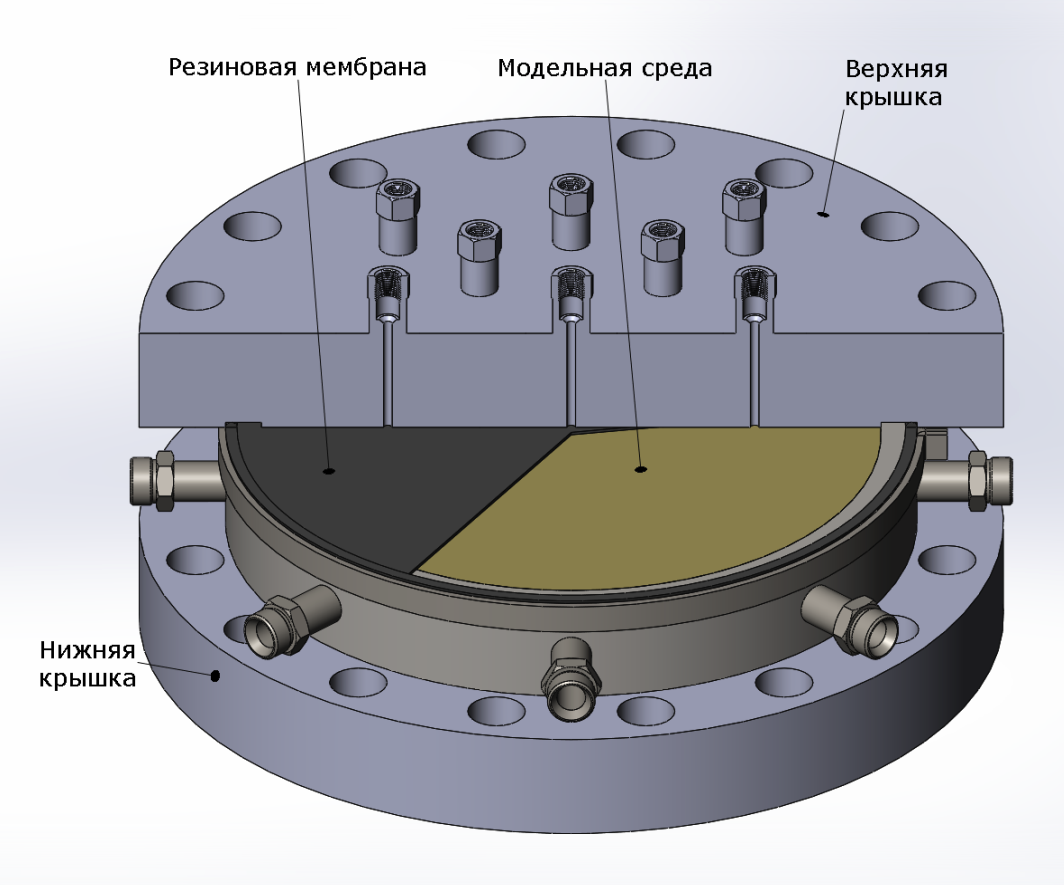
\epsfig{file=figs/picts/1, width=.6\textwidth}
\end{center}
\caption{Схема плоской модельной установки}\label{device:pict}
\end{figure}

Основные детали установки изготовлены из нержавеющей стали. Крышки размещаются на станине, что позволяет свободно их переворачивать и перемещать верхнюю крышку в свой ложемент. Это дает возможность проводить необходимые операции, связанные с подготовкой и проведением экспериментов, несмотря на значительную массу составных частей установки (масса крышек превышает 160 кг). Фотографии общего вида установки представлены на рисунках~\ref{device1:pict}.

\begin{figure}[hb]
\begin{center}
\begin{tabular}{cc}
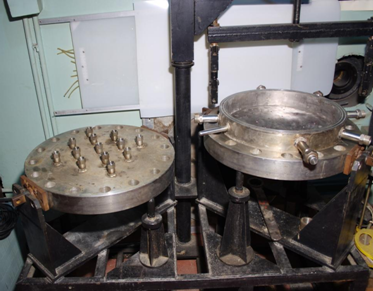
\epsfig{file=figs/picts/2, height=6cm} &
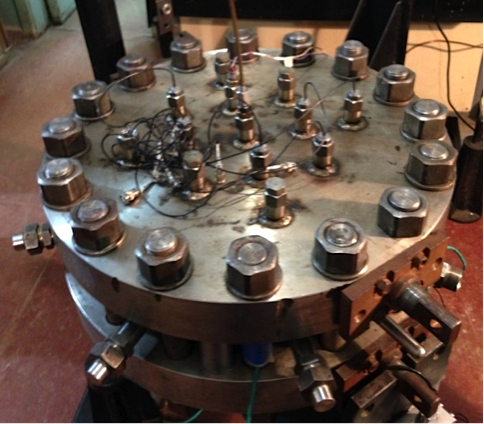
\epsfig{file=figs/picts/3, height=6cm} 
\end{tabular}
\end{center}
\caption{Общий вид экспериментальной установки}\label{device1:pict}
\end{figure}

Перед началом эксперимента в установку заливается гипс. Затвердевая, он образует модельную среду. Верхняя крышка отделена от образца резиновой мембраной. По периметру мембраны расположены резиновое кольцо и опорный хомут, которые создают герметичное пространство между мембраной и крышкой (рис. ~\ref{device:pict}). Это пространство заполняется водой под давлением, что позволяет моделировать литостатическое давление в модели коллектора. Давление над мембраной поддерживается при помощи разделительного цилиндра, верхняя часть которого заполнена сжатым азотом под необходимым давлением, а нижняя водой. 

Горизонтальное нагружение модели обеспечивается с помощью герметичных камер, расположенных на поверхности боковой стенки. Фотография установки (вид сверху) с боковыми камерами представлен на рисунке ~\ref{device2:pict}. Камеры изготовлены из листовой меди толщиной 0,3~мм. Внутренняя полость камер имеет толщину 3~мм, высота камеры на 2~мм меньше высоты боковой стенки. Длина дуги камеры составляет примерно $80^\circ$. Патрубок камеры через герметичное уплотнение выводится из боковой стенки наружу. Камеры зафиксированы на боковой поверхности кольца с помощью силиконового герметика. Боковое нагружение осуществляется за счет закачки газа или жидкости в попарно противоположные камеры.

\begin{figure}[hb]
\begin{center}
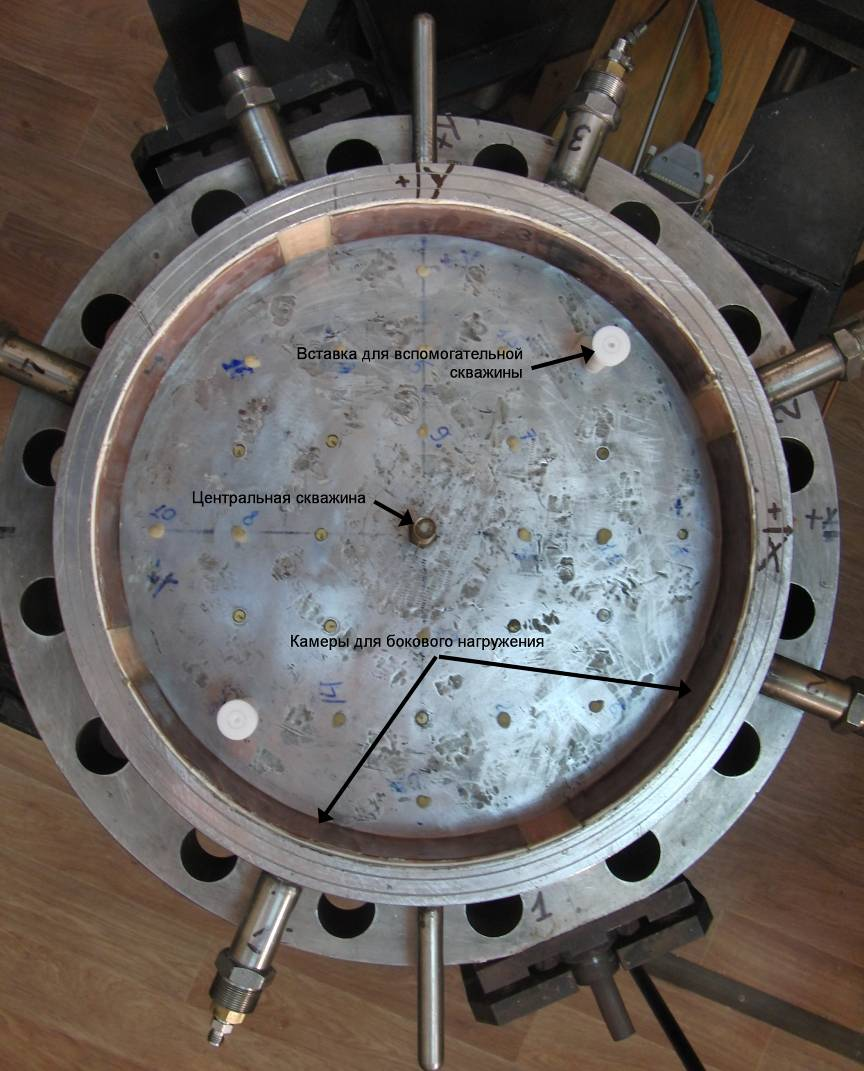
\epsfig{file=figs/picts/4, width=.4\textwidth}
\end{center}
\caption{Фотография установки: вид сверху}\label{device2:pict}
\end{figure}

В обеих крышках и в боковине просверлены сквозные технологические отверстия диаметром 6~мм, оснащенные с внешней стороны приваренными резьбовыми штуцерами. В верхней крышке находится 29 отверстий, в нижней~---13, в боковине~---6. Эти отверстия могут использоваться как для монтажа различных датчиков, так и для обеспечения отбора или закачки флюида в коллектор. Поровое давление в модели измеряется через технологические отверстия, расположенные в нижней крышке установки, с помощью тензопреобразователей. Технологические отверстия заполняются водой и перед заливкой гипса закрываются поролоновыми вкладышами. Вкладыши на 5~мм выступают над поверхностью нижнего основания и после заливки гипса оказываются вмонтированы в него, обеспечивая передачу порового давления к тензопреобразователям. Схема расположения датчиков показана на рисунке~\ref{device3:pict}.

\begin{figure}[hb]
\begin{center}
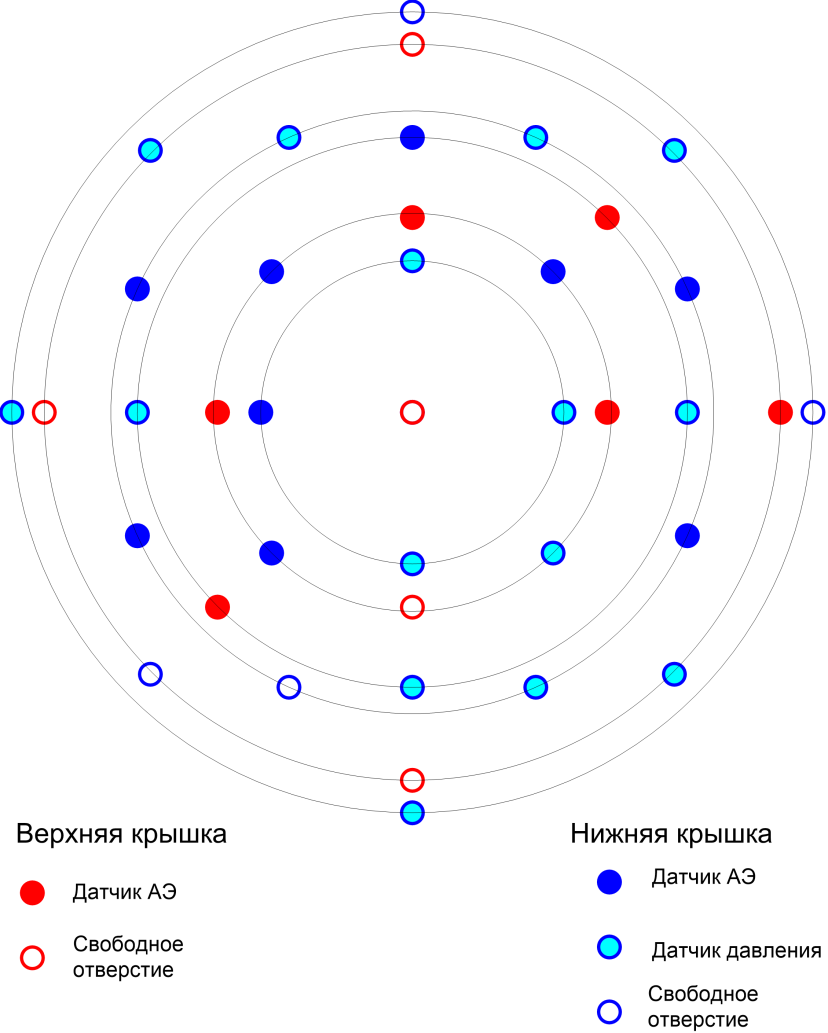
\epsfig{file=figs/picts/5, width=.5\textwidth}
\end{center}
\caption{Схема расположения датчиков в нижней и верхней крышках}\label{device3:pict}
\end{figure}

Вспомогательные скважины, необходимые для прокачки насыщенного раствора сульфата кальция (гипса) через образец и для создания поля порового давления в нем, формируются при отливке образца путем помещения в него заранее вставок из фторопласта диаметром 15~мм в центрально симметричные технологические отверстия (рисунок~\ref{device2:pict}). После затвердевания гипса вставки вынимаются, а сами образовавшиеся скважины закрываются фторопластовыми крышками.

Центральная скважина представляет собой латунную трубку диаметром 16~мм, которая герметично вставляется в нижнюю крышку установки. Трубка имеет возможность свободно вращаться вокруг вертикальной оси, позволяя ориентировать затравку трещины гидроразрыва пласта (ГРП) в заданном направлении. Верхний торец трубки закрыт винтовой пробкой. В средней части трубки проделана вертикальная прорезь, в которую вставляется сложенная вдвое тонкая латунная сетка, служащая затравкой трещины ГРП. Размер лепестков сетки составляет 8х8~мм. Углы лепестков срезаны примерно на 2~мм. После заливки гипса мы получаем обсаженную скважину с перфорированной стенкой и затравкой трещины ГРП.

Эксперименты, как правило, проводятся на третьи сутки после заливки гипса, когда высохнет гипс. После сборки экспериментальной установки модель нагружается небольшим вертикальным давлением (1~МПа), затем задается необходимое давление в боковых камерах. После этого вертикальное давление поднимается до рабочего значения. Перед началом эксперимента проводится дополнительное насыщение гипсового образца жидкостью под постоянным давлением закачки около 1~МПа на технологической нагнетательной скважине. Критерием завершения процесса насыщения служит стабилизация расхода на добывающей скважине и давлений в точках измерения порового давления. Обычно насыщение продолжается около 1~часа. Непосредственно после завершения процесса насыщения проводится эксперимент по ГРП.

\subsection{Модельная среда}

Выбор среды, моделирующей коллектор, определяется целью и постановкой решаемых экспериментальных задач. Целью данного исследования является экспериментальное моделирование ГРП с возможностью переноса результатов экспериментов на пластовые условия. Выбор материала модельного образца связан с двумя основными условиями:
\begin{itemize}
\item
критерии подобия, отвечающие за возможность переноса данных с эксперимента на пласт~\cite{cleary1994};
\item
технологические факторы, связанные с возможностью изготовления экспериментальных образцов.
\end{itemize}
С этой точки зрения смесь на основе гипса с добавкой портландцемента является хорошим выбором. Хорошая текучесть смеси и отсутствие усадки при затвердевании позволяет добиться плотного контакта со стенками установки. Для замедления "схватывания" гипса в воду для приготовления смеси добавляется лимонная кислота в концентрации 2~г/дм$^3$.

В рассматриваемых далее экспериментах среда обладает следующими свойствами.
\begin{description}
%
\item $\nu_\text{dyn} \;\;\,  = 0.25$~-- динамический коэффициент Пуассона,
\item $\nu_\text{st} \;= 0.2$~-- статический коэффициент Пуассона,
\item $E_\text{dyn} \,\,    = 7.5 \times 10^{9}\;$  [Па]~-- динамический модуль Юнга, 
\item $E_\text{st} \,\,    = 3.7 \times 10^{9}\;$  [Па]~-- статический модуль Юнга, 
\item $k \;\;\,    = 2.4 \;\,$  [мД]~-- коэффициент абсолютной проницаемости пласта.

%
\end{description}

Описание экспериментов по определению данных прочностных и фильтрационных характеристик образца можно найти  в~\cite{trimonova2017, trimonova2018}. 

\subsection{Описание эксперимента}

В настоящем разделе приведено описание одного из экспериментов. Эксперимент проводился без гидроразрыва пласта для  проверки теории однофазной фильтрации на кривых падения давления. Для этого во вспомогательные скважины сначала закачивался растрор гипса с целью насыщения образца и создания в нем стационарного поля порового давления, после чего давление в нагнетательной скважине сбрасывалось. Соответственно поровое давление в датчиках начинало спадать, и это фиксировалось в течение всего процесса падения давления. Давления в датчиках записывалось каждые 0.01 секунды. 

Для создания этого эксперимента перед заливкой гипса на дно установки фиксировались вспомогательные скважины в точках с координатами [( 0.057, 0.127 ), (-0.057, -0.127)] и центральная скважина. На дно установки монтировались датчики давления согласно рисунку 4 в точках с координатами [(0.057, -0.127), (0.07, 0.0), (-0.057, 0.127), (0.0, 0.127), (0.0, -0.185), (0.065, 0.065), (-0.121, 0.121), (0.0, 0.07), (0.121, 0.121), (0.127, 0.0), (0.0, -0.07), (0.0, 0.0), (-0.185, 0.0)].  Измеренное в датчиках давление соответствовало давлению на расстоянии 4 мм от дна образца. Далее в установку заливался гипс и высушивался в течение 2-3 дней. После затвердевания образца вспомогательные боковые скважины удалялись. Далее, как упоминалось выше, сверху на образец подавалось давление (20~атм, где 1~атм~=~101335~Па), имитируя литостатическое давление. Давление в боковых камерах не задавалось. После этого во вспомогательную скважину с координатами центра $(0.057, 0.127 )$ и радиусом 7.5~мм закачивался раствор гипса с постоянным давлением (14.5~атм). Другая скважина была соединена с атмосферой. Насыщение образца продолжалось до установления в нем стационарного режима. Установление режима определялось по давлению в  центре образца, в точке с координатами $(0, 0)$. Когда давление в ней достигало значения, равного полусумме давлений, заданных в боковых скважинах. После этого раствор в нагнетательную скважину переставал подаваться. Кривые давления в датчиках порового давления фиксировались в течение всего эксперимента (рисунок~\ref{device4:pict}) . Длительность всего эксперимента составила примерно 220~мин. 

\begin{figure}[hb]
\begin{center}
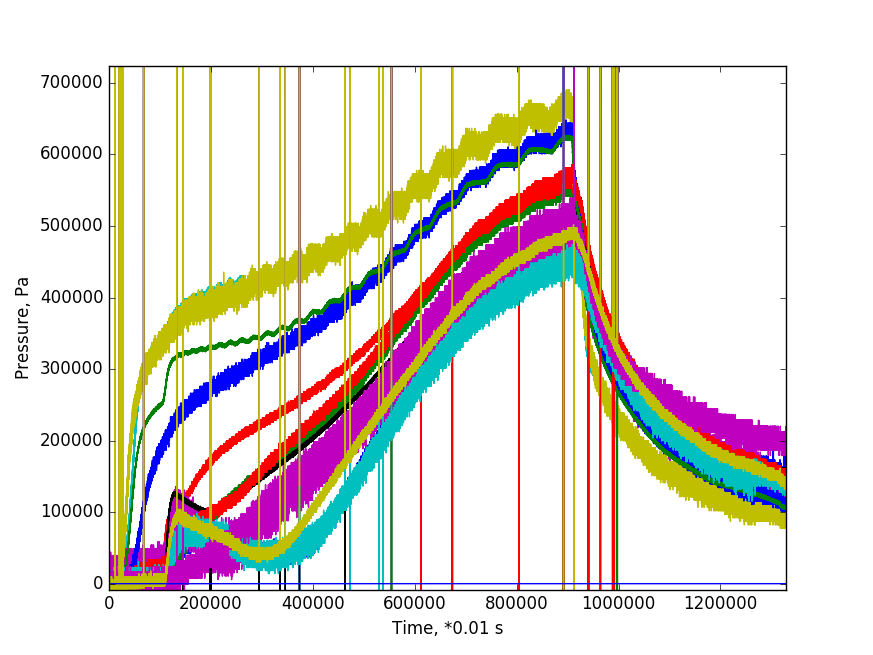
\epsfig{file=figs/picts/6, width=.6\textwidth}
\end{center}
\caption{Кривые давления в датчиках порового давления}\label{device4:pict}
\end{figure}





\section{Результаты расчетов}
\label{sec:results}
%
%
% problem.tex
% 
% Постановка задач и результаты расчетов
% 

\settocdepth{subsection}

В настоящем разделе представлены результаты численных расчетов, проведенных с помощью разработанного авторами
программного комплекса. Рассмотрены как валидационные, так и прикладные задачи, встречающиеся при моделировании
течений в пороупругих средах.

Параметры пороупругой среды соответствуют песчанику из Берейского месторождения~\cite{detournay_1993},
насыщенному водой:
%
\begin{description}
%
\item $\nu \;\;\,  = 0.20$~-- дренированный коэффициент Пуассона,
\item $\nu_u \;= 0.33$~-- недренированный коэффициент Пуассона,
\item $B \;\,    = 0.62$~-- коэффициент Скемптона порового давления,
\item $b \;\;\;    = 0.79$~-- коэффициент Био,
\item $\varphi \;\;= 0.19$~-- пористость пласта,
\item $M \,\,    = 1.3 \times 10^{10}$  [Н/м$^2$]~-- модуль Био,
\item $G \,\,\,    = 6.0 \times 10^9\;\,$  [Н/м$^2$]~-- модуль сдвига,
\item $E \,\,    = 1.4 \times 10^{10}\;$  [Н/м$^2$]~-- дренированный модуль Юнга, 
\item $K \,\,    = 8.0 \times 10^9\;\,$  [Н/м$^2$]~-- дренированный объемный модуль сжатия, 
\item $E_u   = 1.6 \times 10^{10}\,$  [Н/м$^2$]~-- недренированный модуль Юнга, 
\item $K_u   = 1.6 \times 10^{10}\,$ [Н/м$^2$]~-- недренированный объемный модуль сжатия,
%\item $K_s   = 3.6 \times 10^{10}\,$ [Н/м$^2$]~-- объемный модуль сжатия породы,
%\item $K_f   = 3.3 \times 10^9\;\,$  [Н/м$^2$]~-- объемный модуль сжатия флюида,
\item $k \;\;\,    = 1.9 \times 10^2\;\,$  [мД]~-- коэффициент абсолютной проницаемости пласта,
\item $\mu \;\;\,  = 1.0 \times 10^{-3}$  [Па$\cdot$с]~-- вязкость флюида,
\item $\rho_f^0 \;\;\,  = 1.0 \times 10^{3}\;\,$ [кг/м$^3$]~-- плотность флюида.
%
\end{description}
%

В настоящей работе в качестве первичных переменных используются $E, \nu, b, M, \varphi, k, \mu , \rho_f^0$,
остальные величины выражаются через них с помощью известных соотношений~\cite{coussy_2004}. Также полагается, что массовые силы отсутствуют.

\newpage

\subsection{Задача о мгновенном точечном источнике}

Данная задача является одной из простейших задач пороупругости, но составляет, на наш взгляд, полезный тестовый пример.
Рассмотрим бесконечную невозмущенную пороупругую среду.
В начальный момент времени происходит впрыскивание флюида массы $M_f$ с объемом $V_f = M_f/\rho^0_f$ в точку,
расположенную в начале системы координат, что мгновенно приводит к деформации попроупругой среды.
В такой постановке решение задачи, очевидно, обладает радиальной симметрией.

%Данная задача имеет аналитическое решение.
%За счет симметрии, уравнение на $v_f$ принимает вид \cite{coussy_2004}
%\begin{equation}
  %\dfdx{(r v_f)} t = c_f \dfdx{^2(r v_f)}{r^2},
%\end{equation}
%где $c_f$ ~--- коэффициент фильтрации
%$$
%c_f = M \frac{k}{\mu} \times \frac{K + \frac 43\nu}{K_u + \frac 43 \nu}.
%$$
%В итоге получаем \cite{coussy_2004}
%$$
%v_f = \frac{V_f}{(4\pi c_f t)^{\frac32}}\exp\left(- \frac{r^2}{4c_ft} \right),
%$$

Аналитическое решение данной задачи записывается в виде~\cite{coussy_2004}:
%
\begin{gather}
\label{eq:prdot}
p(r,t) = %M \frac{K + \frac 43\mu}{K_u + \frac 43 \mu}
\frac{c_f V_f}{(4\pi c_f t)^{\frac32}(k/\mu)}\exp\left(-\frac{r^2}{4c_ft} \right),\\
%\end{equation}
%
%\begin{equation}
\label{eq:urdot}
u_r(r,t) = \frac{3 b M}{3K_u + 4 \nu} \cdot \frac{V_f}{4\pi r^2} \,g\left(\frac r{\sqrt{c_f t}}\right),
\end{gather}
где
\begin{equation}
\label{eq:cf}
c_f = M \,\frac{k}{\mu} \cdot \frac{3K + 4\nu}{3K_u + 4\nu},
\end{equation}
%
\begin{equation*}
g(\lambda) = \erf\left(\frac\lambda2\right) - \frac\lambda{\sqrt\pi}\exp\left(-\frac{\lambda^2}4\right), \quad
\erf(x) = \frac 2{\sqrt \pi} \int\limits_0^x e^{-\lambda^2}\,d\lambda.
\end{equation*}

 %и $\erf(x)$ --- интеграл ошибок
 %и в декартовой системе координат $\{r_i\}$
%$$
%u_i = u_r \frac{r_i}{r}.
%$$

Для расчетов использовалась область в форме куба со стороной $L_r$,
в центре которого впрыскивался флюид. Схематично постановка задачи представлена на рис.~\ref{fig:immdot}.
Конкретные значения используемых для расчетов параметров приведены в табл.~\ref{tab:immdot}.
На границе расчетной области давление и перемещение задавались согласно 
точному решению~\eqref{eq:prdot}--\eqref{eq:urdot}, аналогичным образом
задавалось и начальное распределение на момент времени $t_{\text{start}}$.
%
\begin{figure}[h!]
\centering
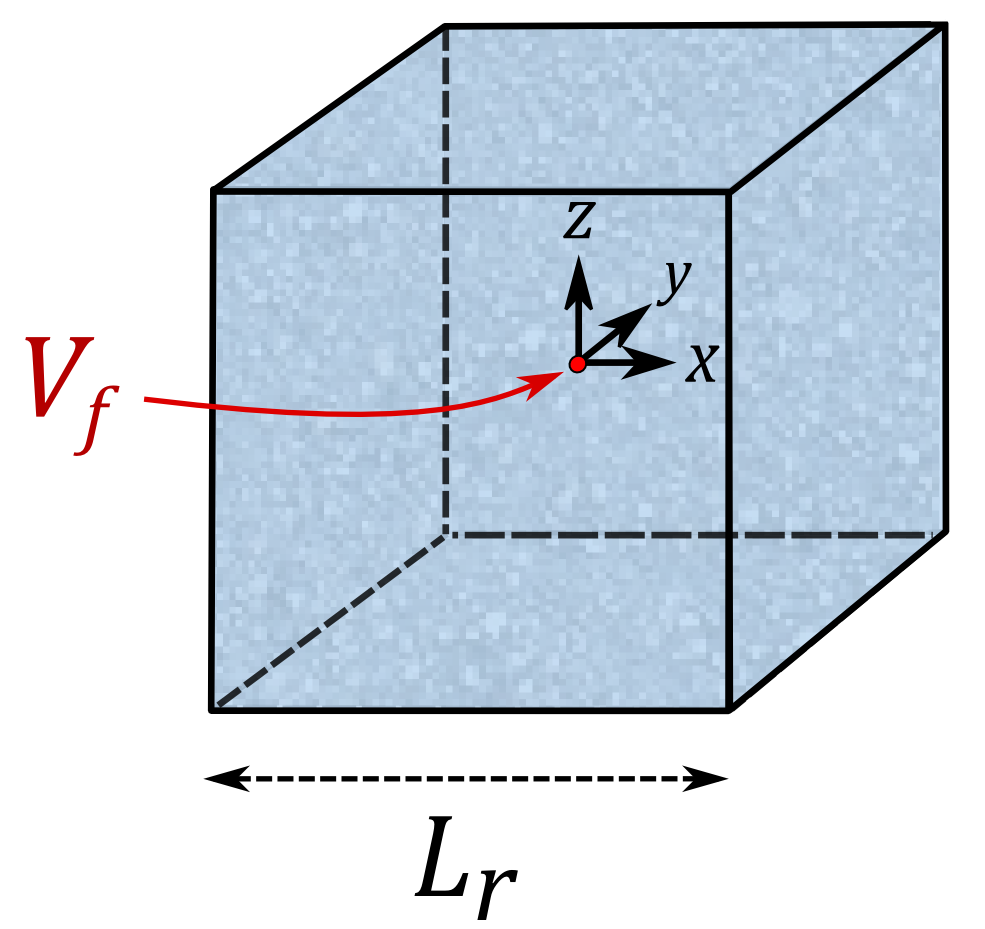
\includegraphics[width=0.45\textwidth]{./figs/immdot.png}
\caption{Схематичный вид задачи о мгновенном точечном источнике.}\label{fig:immdot}
\end{figure}
% 
%
%%
\begin{table}[h!]
\centering
%
\renewcommand{\arraystretch}{1.5}
\renewcommand{\tabcolsep}{6 pt} 
\begin{tabular}{|c|c|c|c|c|c|c|}
\hline
$L_r$ & $V_f$ & $t_{\text{start}}$ & $t_{\text{end}}$ & $\Delta t$\\
\hline
 $400.0$ м & $1.0 \text{ м}^3$ & $150.0$ с & $200.0$ с & $1.0$ с\\
\hline
\end{tabular}
%
\caption{Параметры для численного расчета задачи о мгновенном точечном источнике.}\label{tab:immdot}
\end{table}
%%
%
 

В расчетах использовалась тетраэдральная сетка, состоящая из 
$N_{nodes} = 68921$ узлов и $N_{elems} = 256000$ прямоугольных тетраэдров со сторонами $h_x = h_y = h_z = 1.0$ м.

В качестве величин для сравнения используются нормированные значения $\overline{p}$, $\overline{u}_r$:
%
\begin{equation*}
%
\overline{p} = \cfrac{p}{p_0}, \quad \overline{u}_r = \cfrac{u_r}{L_r},
%
\end{equation*}
%
где 
\begin{equation}
\label{eq:p0p0}
p_0 = \mu V_f / 2 k.
\end{equation}

Результаты расчетов и точное решение приведены на
рис.~\ref{fig::press_point_mom},
% и \ref{fig::disp_point_mom},
где показаны нормированные давления и перемещения в последовательные моменты времени
$t = 150, \; 165, \; 185, \; 200$ с. Как видно из рисунков, получено
хорошее совпадение с аналитическими результатами на все указанные моменты времени.

\begin{figure}[t!]
\centering
  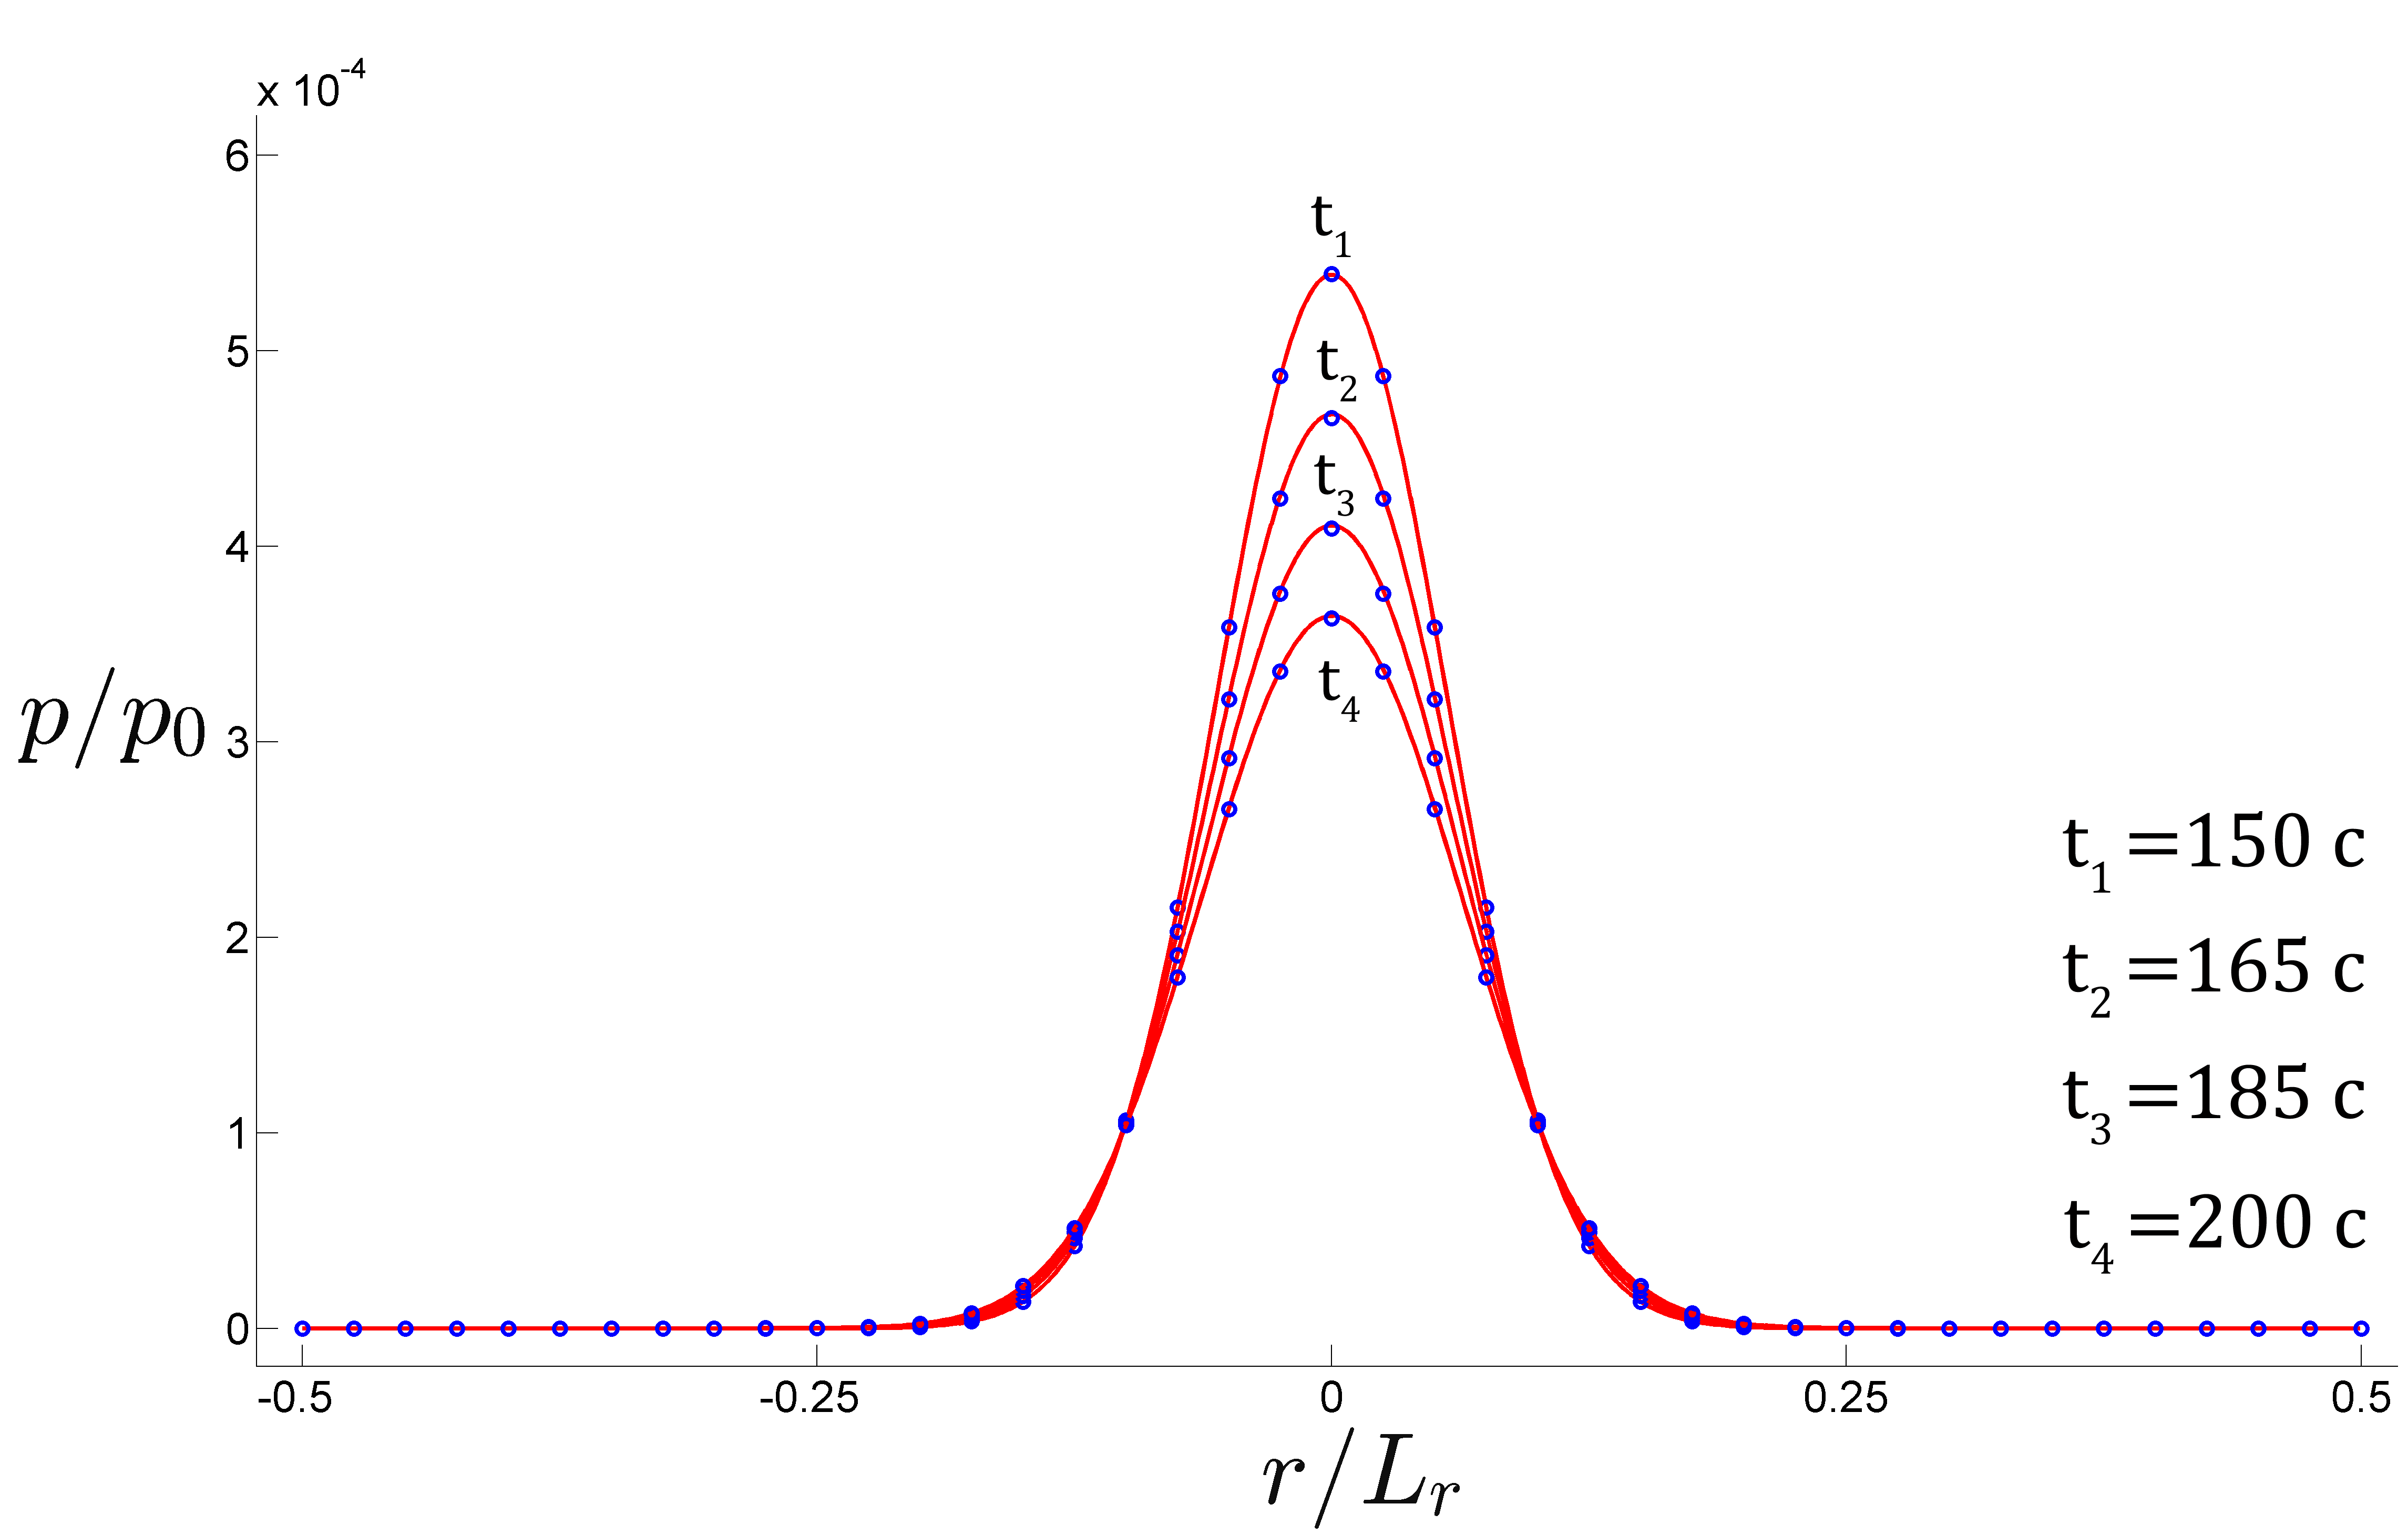
\includegraphics[width=0.8\textwidth]{figs/press_point_mom2.png}\\
  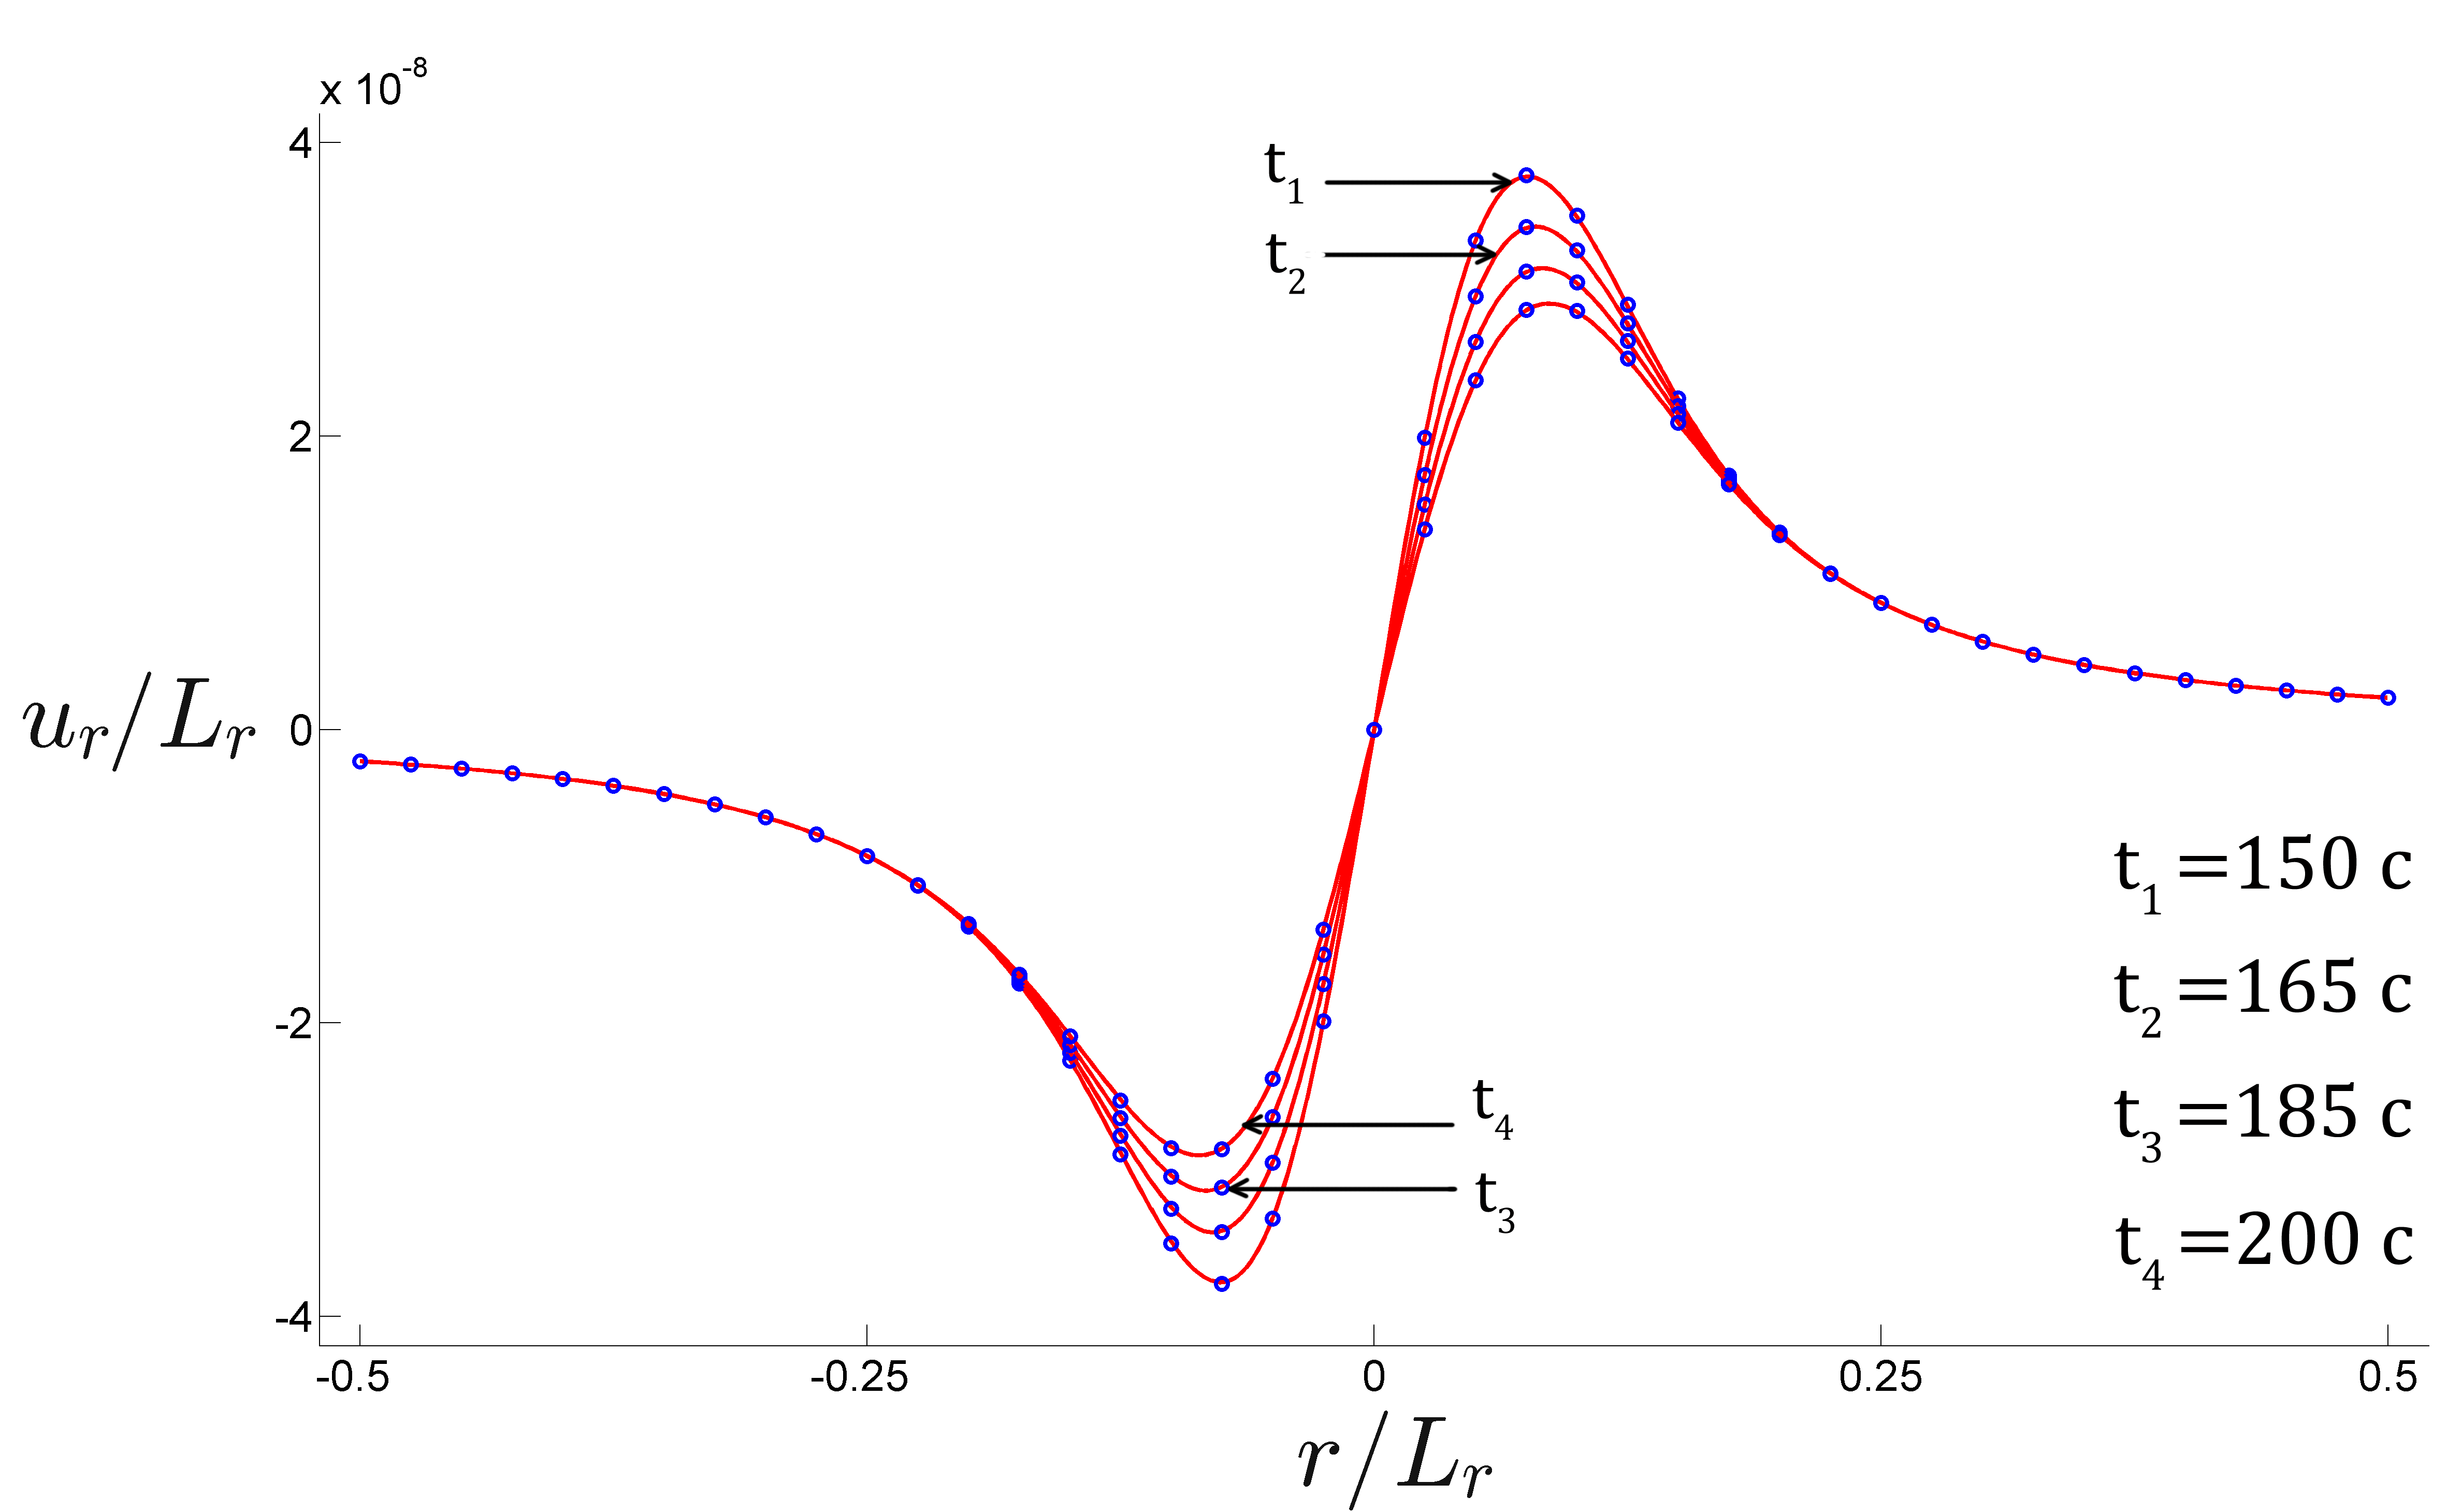
\includegraphics[width=0.8\textwidth]{figs/disp_point_mom2.png}
  \caption{ Задача о мгновенном точечном источнике. Нормированное давление (вверху) и перемещение (внизу) в различные моменты времени: красным
    цветом показано аналитическое решение, синим~--– результаты расчета.}
  \label{fig::press_point_mom}
\end{figure}
%
% \begin{figure}[t!]
% \centering
%   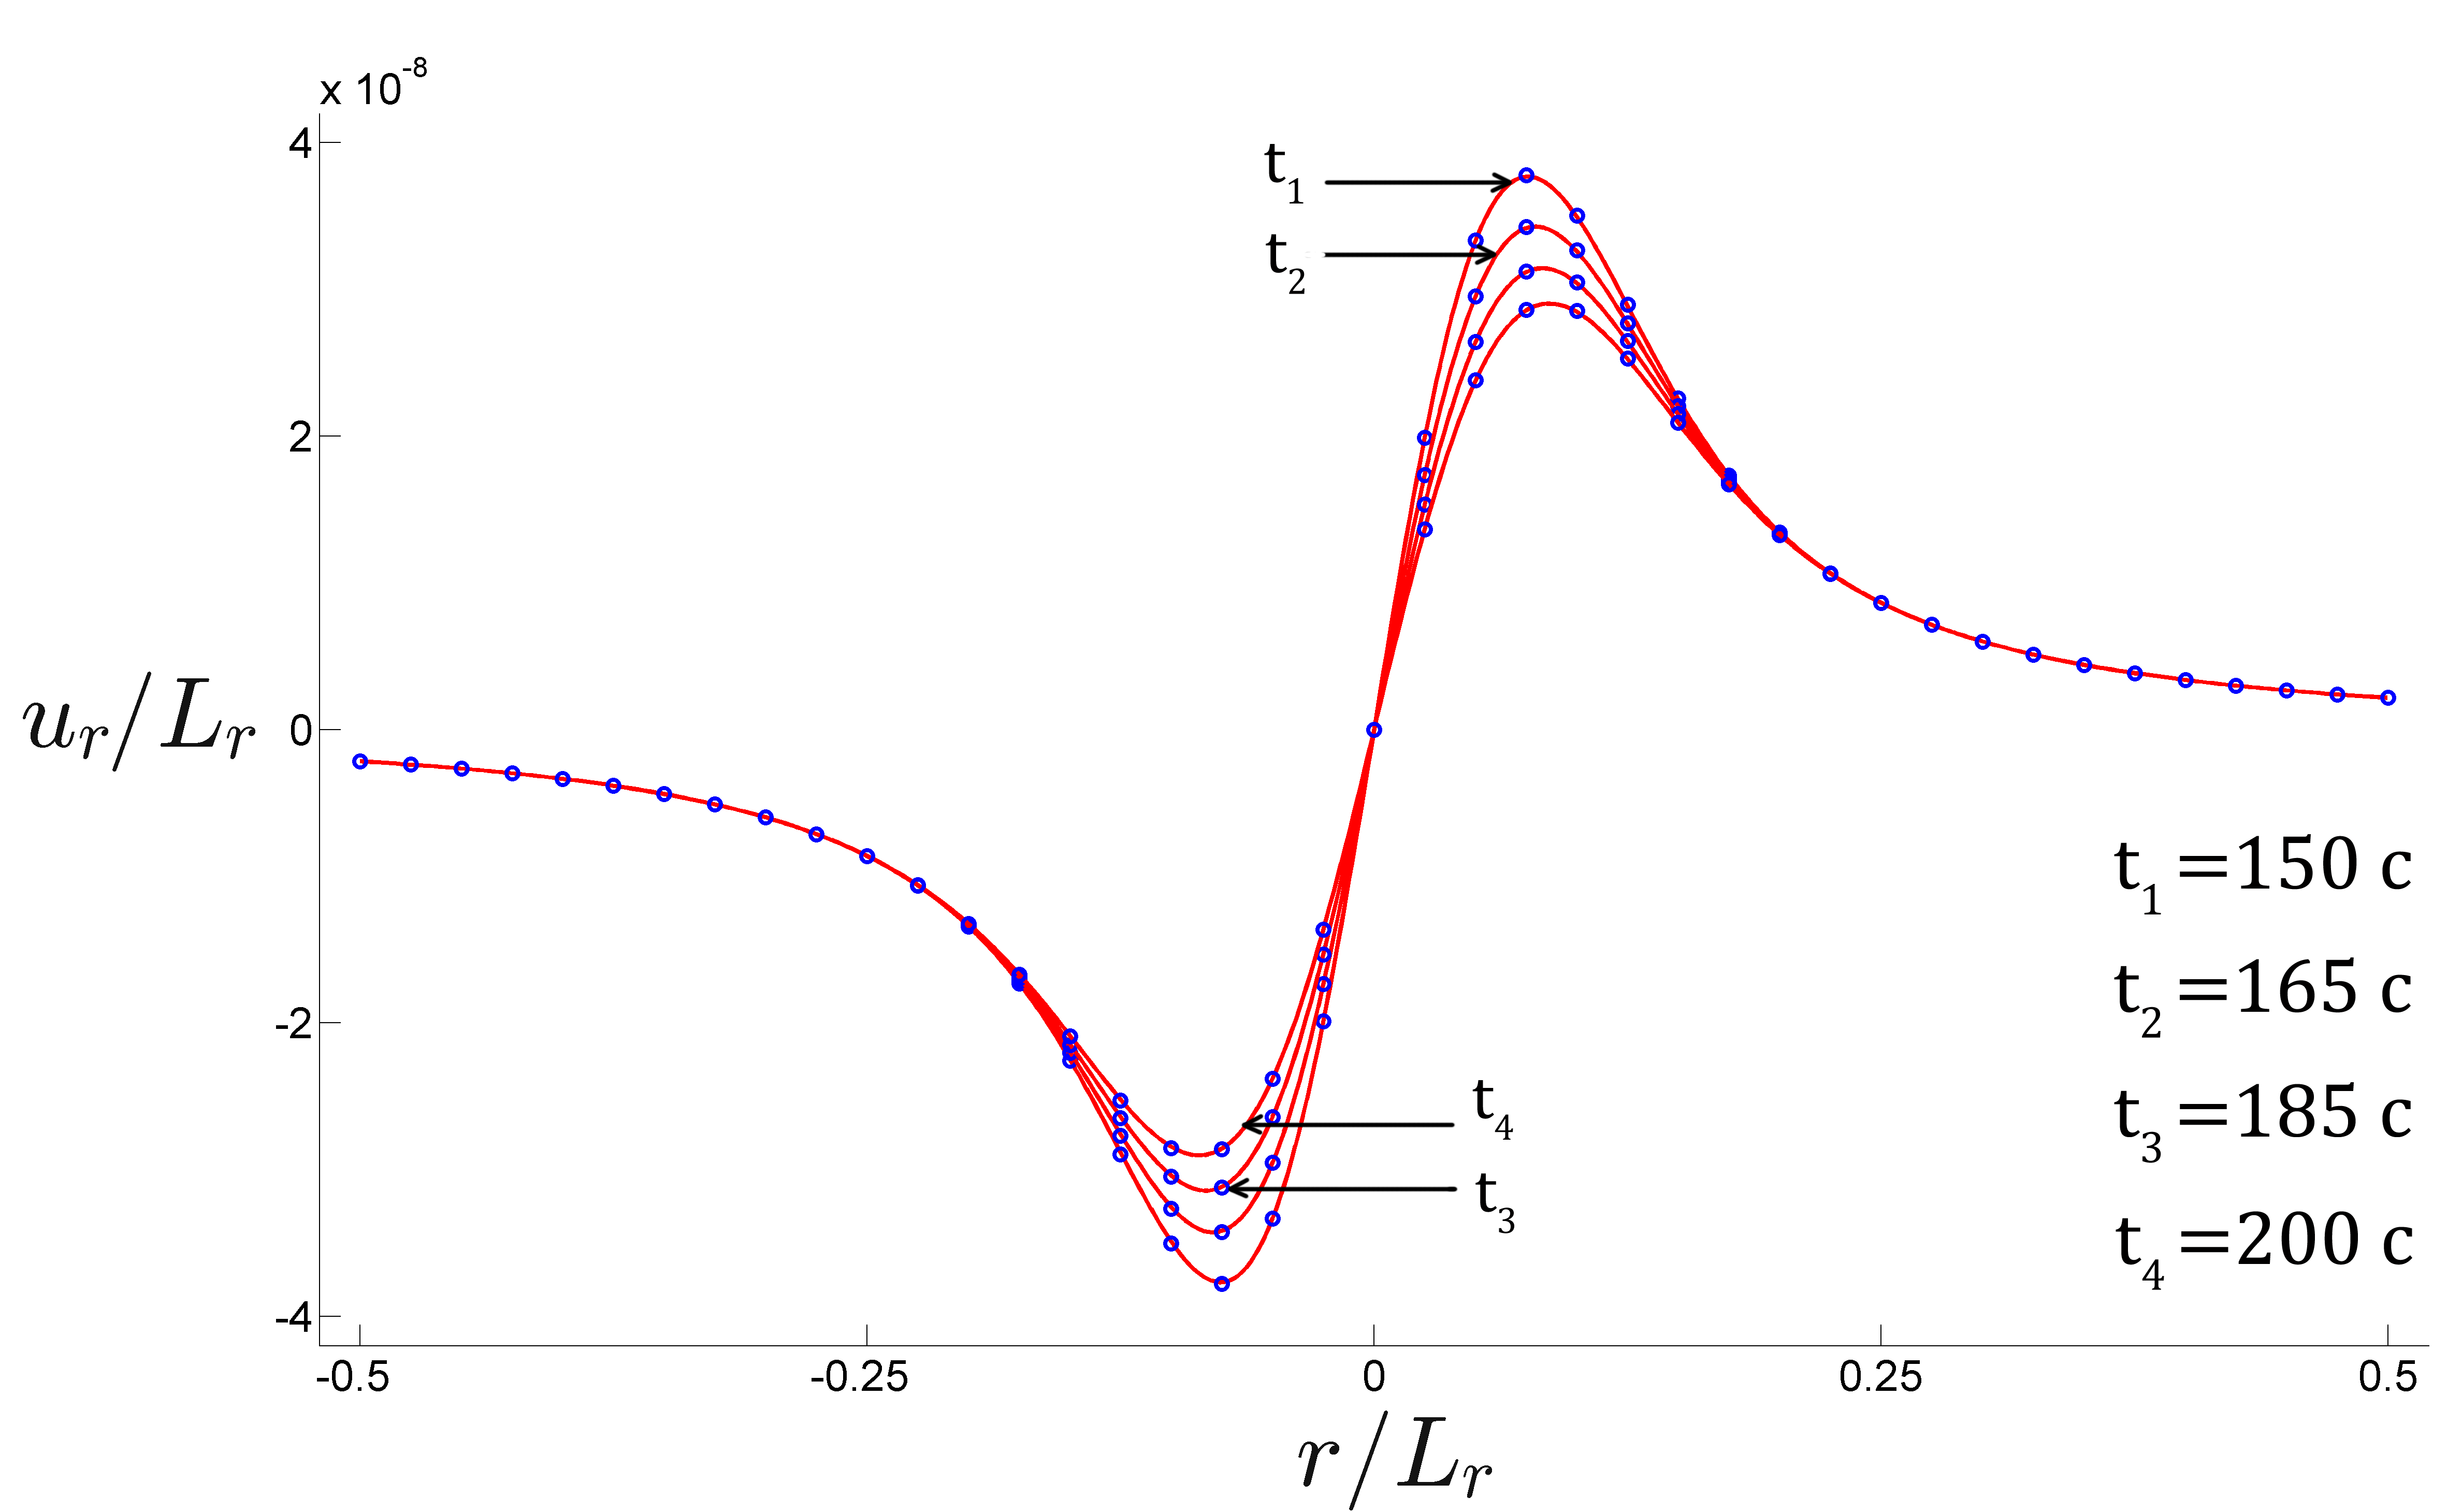
\includegraphics[width=0.8\textwidth]{figs/disp_point_mom2.png}
%   \caption{ Нормированное перемещение в различные моменты времени: красным
%   цветом показано аналитическое решение, синим – результаты расчета}
%   \label{fig::disp_point_mom}
% \end{figure}


%\newpage

\subsection{Задача о мгновенном линейном источнике}
Задача о линейном источнике является простейшей моделью, описывающей скважину в пороупругой среде.
Поэтому расчет этого теста является обязательной валидационной задачей для программных комплексов,
моделирующих течения в пороупругих средах.

Задача ставится следующим образом: в бесконечной невозмущенной
пороупругой среде в момент времени $t=0$ с на некоторой линии
происходит впрыскивание массы флюида с линейной плотностью $M_f$
объемом $V_f = M_f/\rho^0_f$, что мгновенно приводит к деформации
попроупругой среды.  В такой постановке решение задачи, очевидно,
обладает радиальной симметрией.
 
Аналитическое решение задачи записывается следующим образом~\cite{coussy_2004}:
\begin{equation}
\label{eq:immlinep}
%
p(r,t) = \frac{V_f}{4\pi (k/\mu) t} \exp{\left( -\frac{r^2}{4 c_f t}\right)}, \\
%
\end{equation}
%
\begin{equation}
\label{eq:immlinur}
u_r(r,t) = \frac{3bM}{3K_u+4\nu} \cdot \frac{V_f}{2 \pi r} \left[1 - \exp{\left( -\frac{r^2}{4 c_f t}\right)} \right],
\end{equation}
%
%\igma_{rr} = \frac{bM\mu}{K_u+\frac{4}{3}\mu} \frac{V_f}{2\pi r^2} \left[1 - \exp{\left( -\frac{r^2}{4 c_f t}\right)} \right] \\
%
%\sigma_{\theta\theta} = \frac{bM\mu}{K_u+\frac{4}{3}\mu} \frac{V_f}{2\pi r^2} \left[1 - \left(1+\frac{r^2}{2c_f t}\right) \exp{\left( -\frac{r^2}{4 c_f t}\right)} \right] \\
%
%\sigma_{zz} = \frac{bM\mu}{K_u+\frac{4}{3}\mu} \frac{V_f}{2\pi c_f t} \left[1 - \exp{\left( -\frac{r^2}{4 c_f t}\right)} \right]
%\end{eqnarray}
где $c_f$ определяется согласно формуле~\eqref{eq:cf}.

Для расчетов использовалась область с линейными размерами $L_x$, $L_y$, $L_z$,
в центре которой располагался линейный источник,
проходящий через точки с координатами $(0, 0, 0)$ и $(0, 0, L_z)$.
Схематично постановка задачи представлена на рис.~\ref{fig:immline}.
Конкретные значения используемых для расчетов параметров приведены в табл.~\ref{tab:immline}.

На границе расчетной области перемещение задавались согласно 
точному решению~\eqref{eq:immlinep}, для давления на всех границах использовалось условие
нулевого потока $\partial p/ \partial n = 0$. Начальное распределение задавалось
согласно аналитическому решению на момент времени $t_{\text{start}}$.
%
\begin{figure}[t!]
\centering
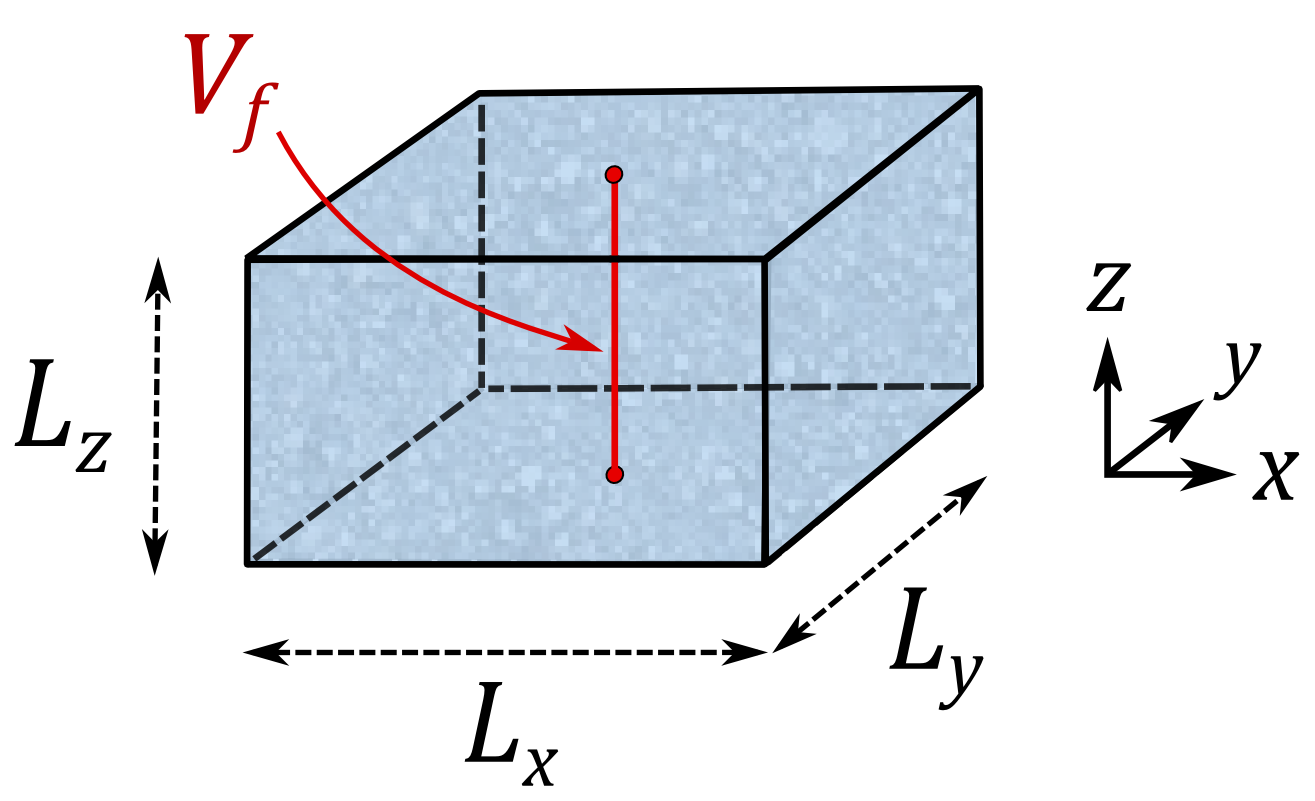
\includegraphics[width=0.65\textwidth]{./figs/immline.png}
\caption{Схематичный вид задачи о мгновенном линейном источнике.}\label{fig:immline}
\end{figure}
% 
%
%%
\begin{table}[h!]
\centering
%
\renewcommand{\arraystretch}{1.5}
\renewcommand{\tabcolsep}{6 pt} 
\begin{tabular}{|c|c|c|c|c|c|c|}
\hline
$L_x$ & $L_y$ & $L_z$ & $V_f$ & $t_{\text{start}}$ & $t_{\text{end}}$ & $\Delta t$\\
\hline
 $400.0$ м & $400.0$ м & $10.0$ м & $1.0 \text{ м}^3$ & $150.0$ с & $200.0$ с & $1.0$ с\\
\hline
\end{tabular}
%
\caption{Параметры для численного расчета задачи о мгновенном линейном источнике.}\label{tab:immline}
\end{table}
%%
%

В расчетах использовалась тетраэдральная сетка, состоящая из 
$N_{nodes} = 5043$ узлов и $N_{elems} = 12800$ прямоугольных тетраэдров со сторонами $h_x = h_y = h_z = 1.0$ м.

В качестве величин для сравнения используются нормированные значения $\overline{p}$, $\overline{u}_r$:
%
\begin{equation*}
%
\overline{p} = \cfrac{p}{p_0}, \quad \overline{u}_r = \cfrac{u_r}{L_r},
%
\end{equation*}
%
где $p_0$ определялось согласно формуле~\eqref{eq:p0p0}, $L_r = L_x = L_y$.
 

Результаты расчетов и точное решение приведены на
рис.~\ref{fig::press_line_mom}
% и \ref{fig::disp_line_mom},
где показаны нормированные давления и перемещения в последовательные моменты времени
$t = 150, \; 165, \; 185, \; 200$ с. Как видно из рисунков, получено
хорошее совпадение с аналитическими результатами на все указанные моменты времени.

\begin{figure}[t!]
\centering
  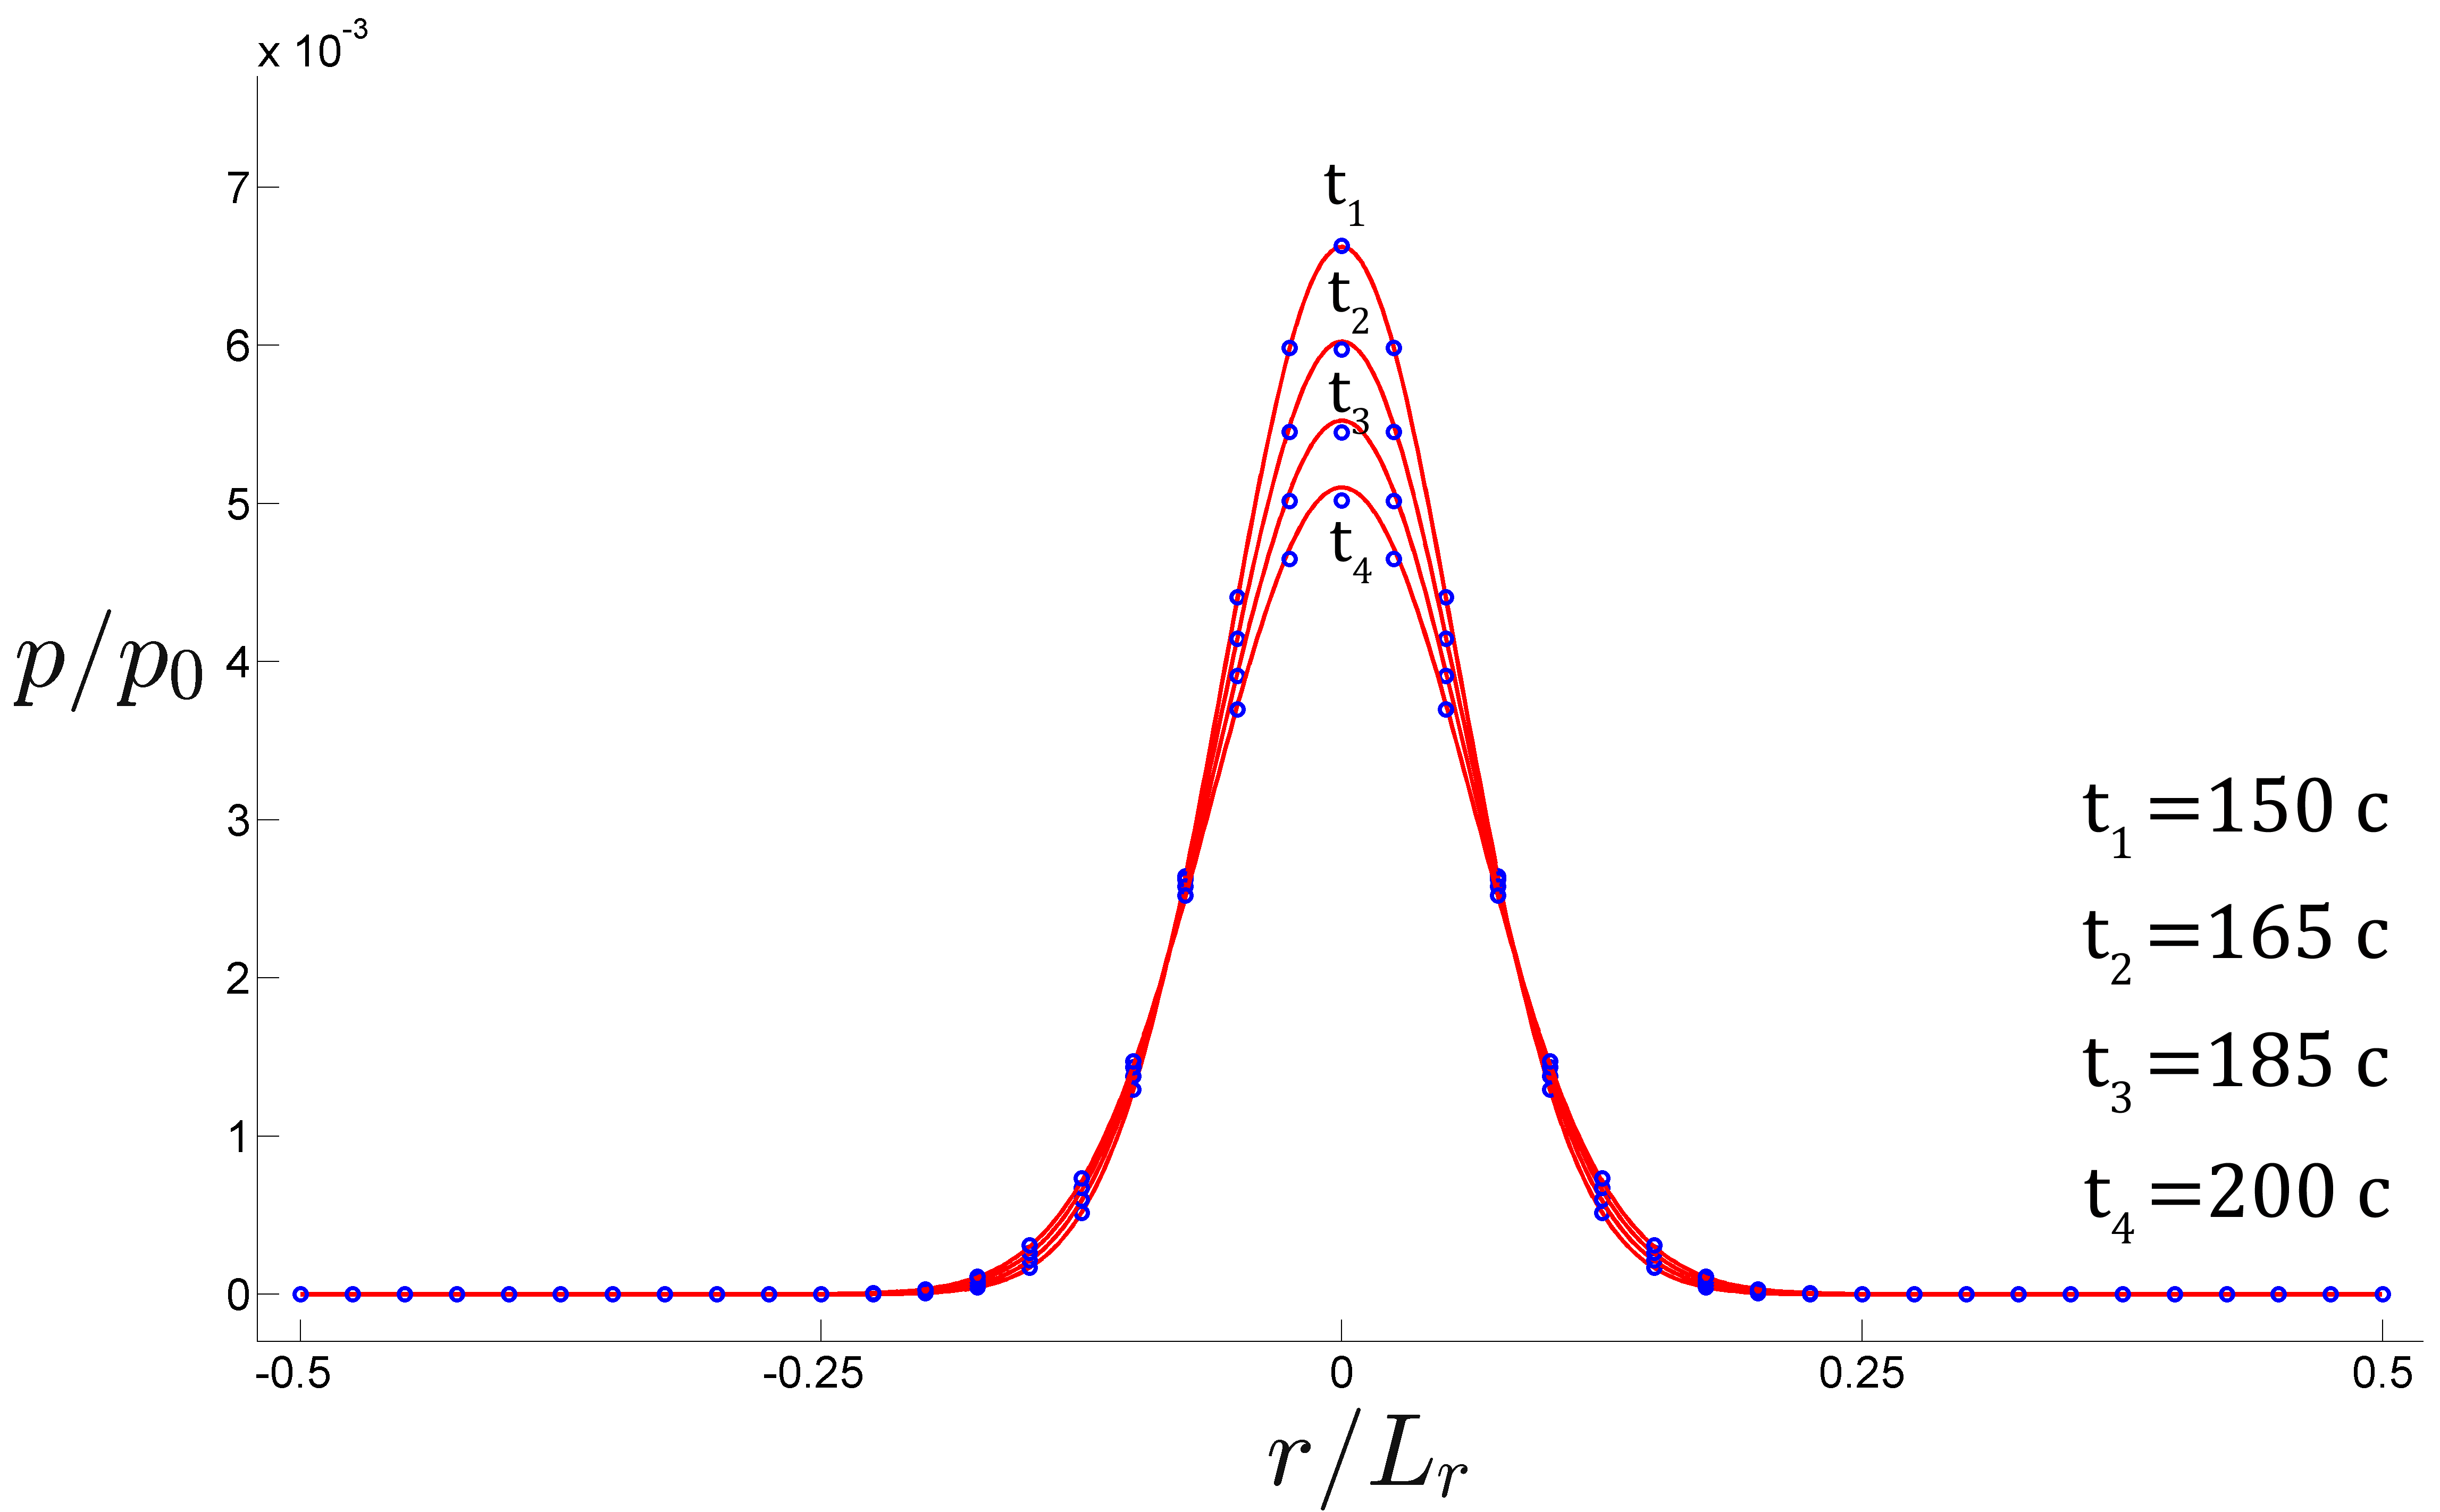
\includegraphics[width=0.8\textwidth]{figs/press_line_mom2.png}\\
  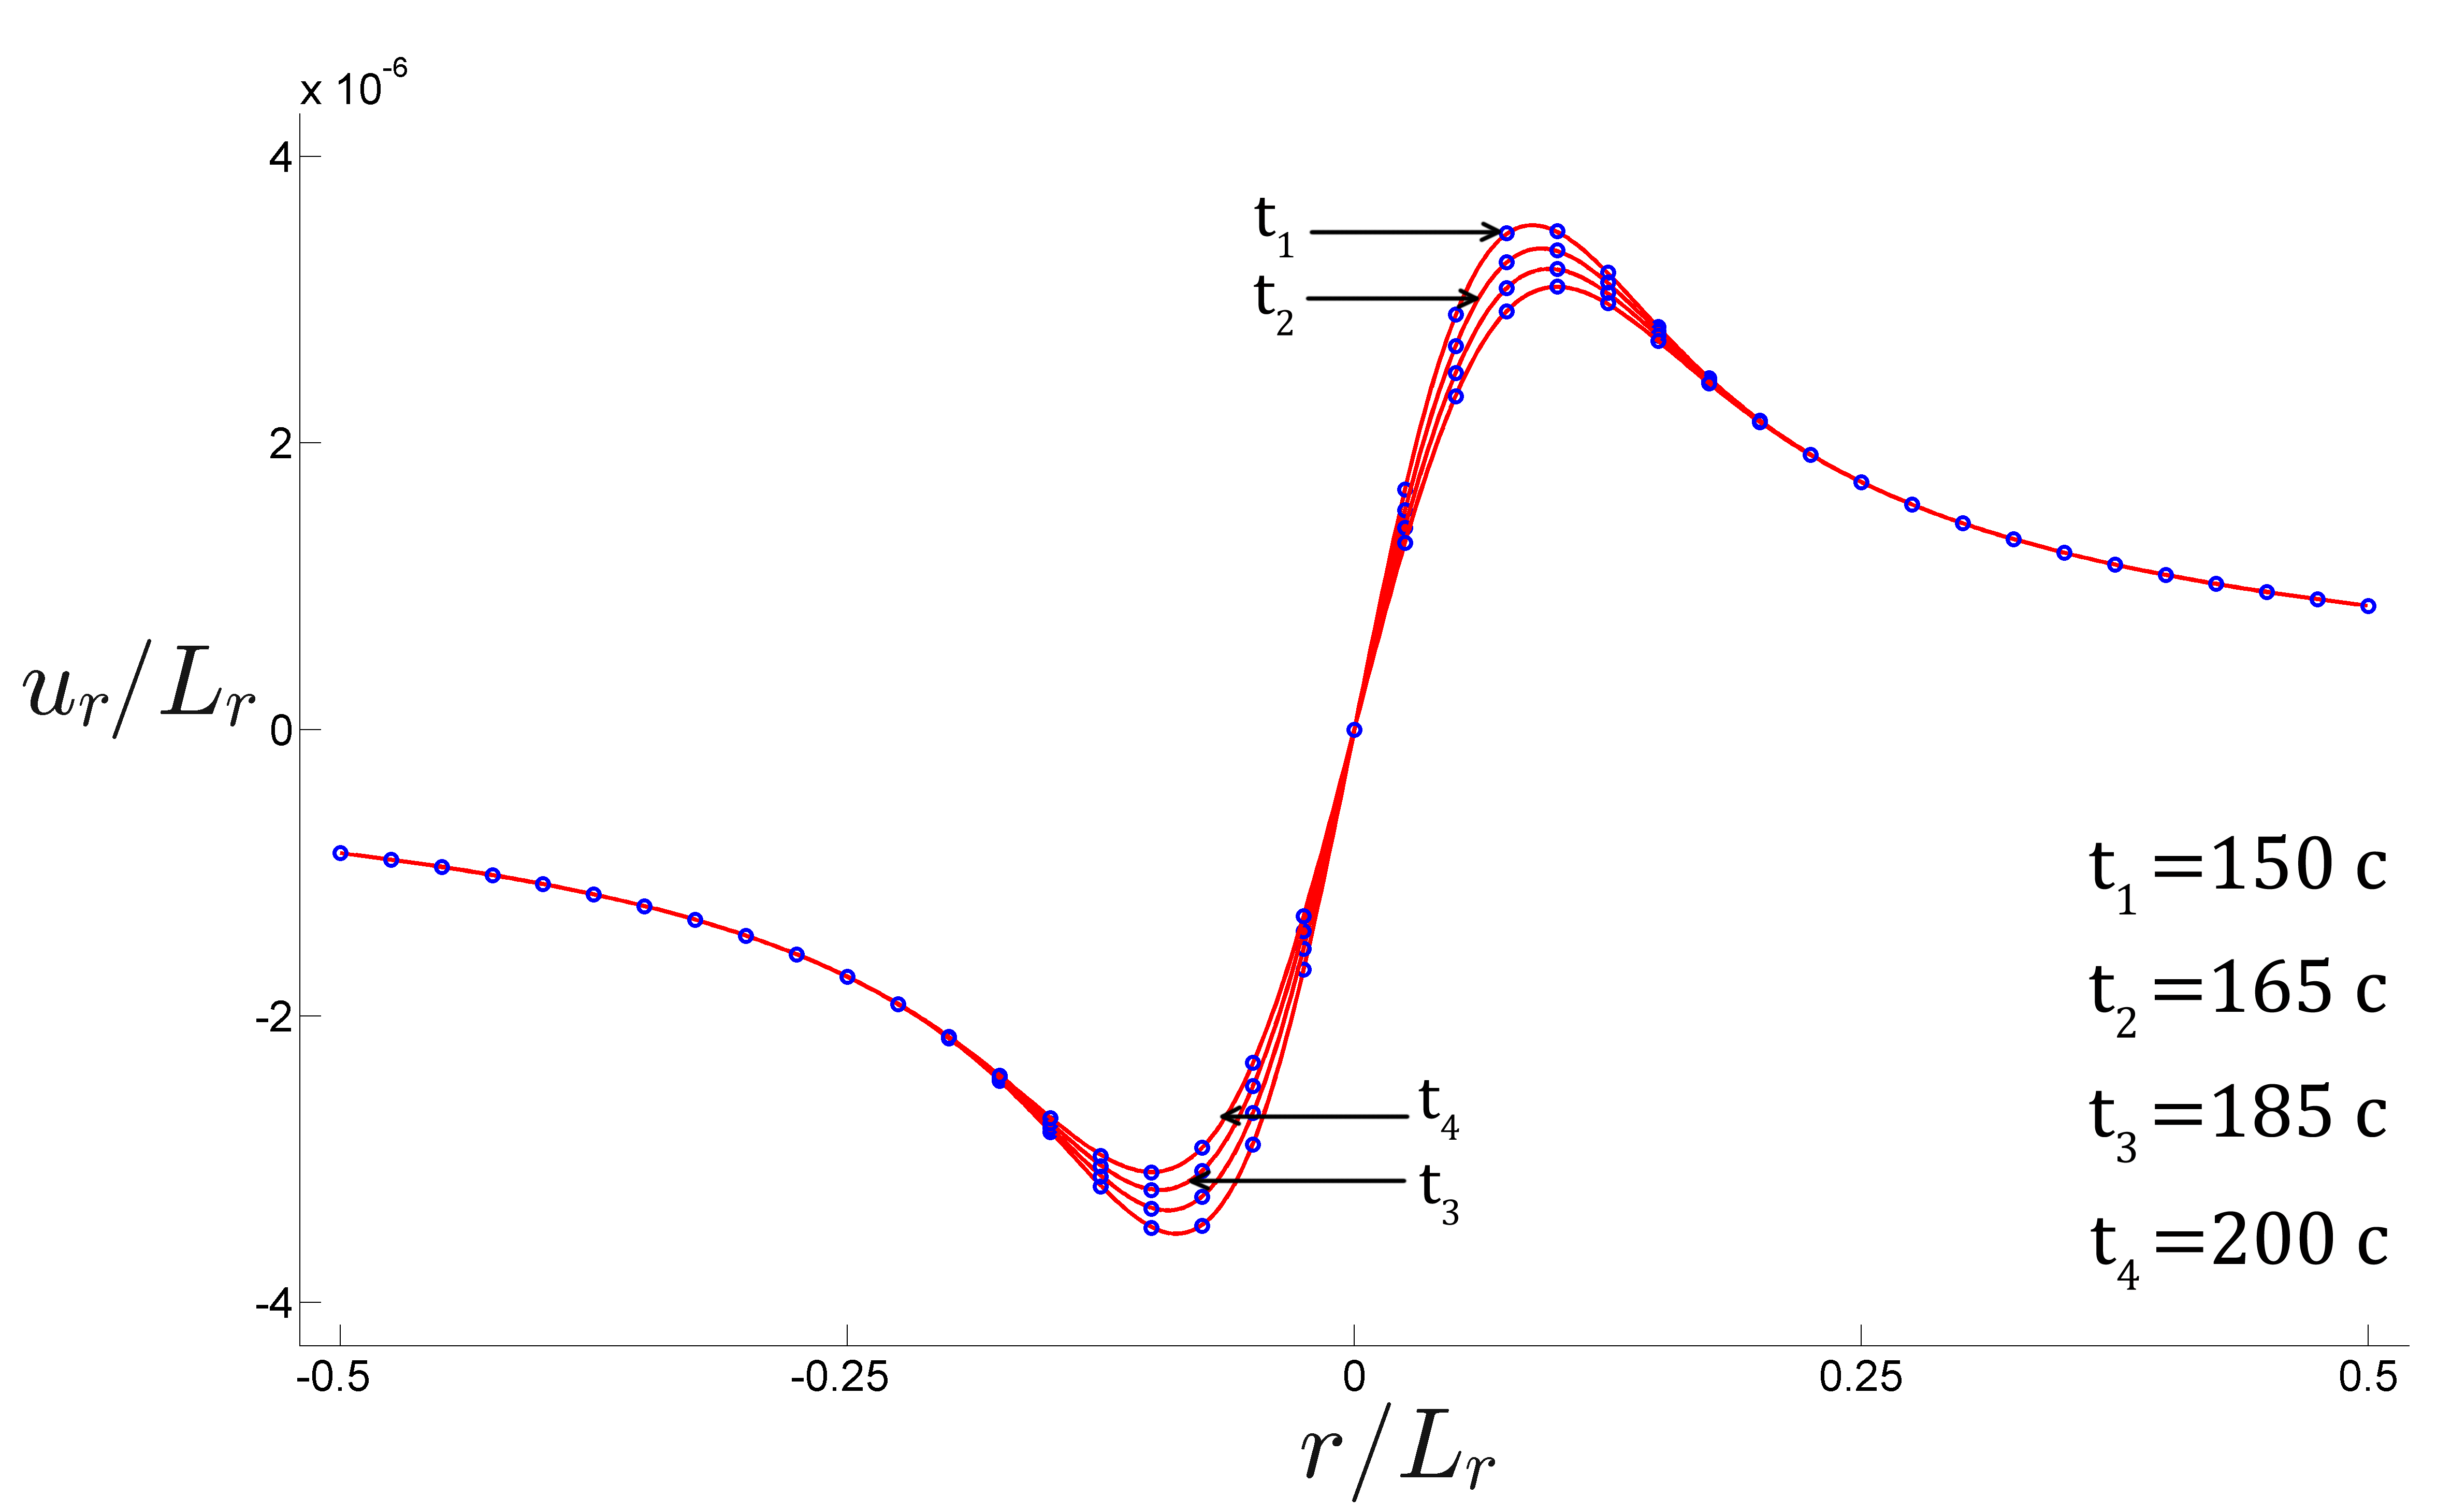
\includegraphics[width=0.8\textwidth]{figs/disp_line_mom2.png}
  \caption{ Задача о мгновенном линейном источнике. Нормированное давление (вверху) и перемещение (внизу) в различные моменты времени: красным
цветом показано аналитическое решение, синим~--– результаты расчета.}
  \label{fig::press_line_mom}
\end{figure}
% %
% \begin{figure}[b!]
% \centering
%   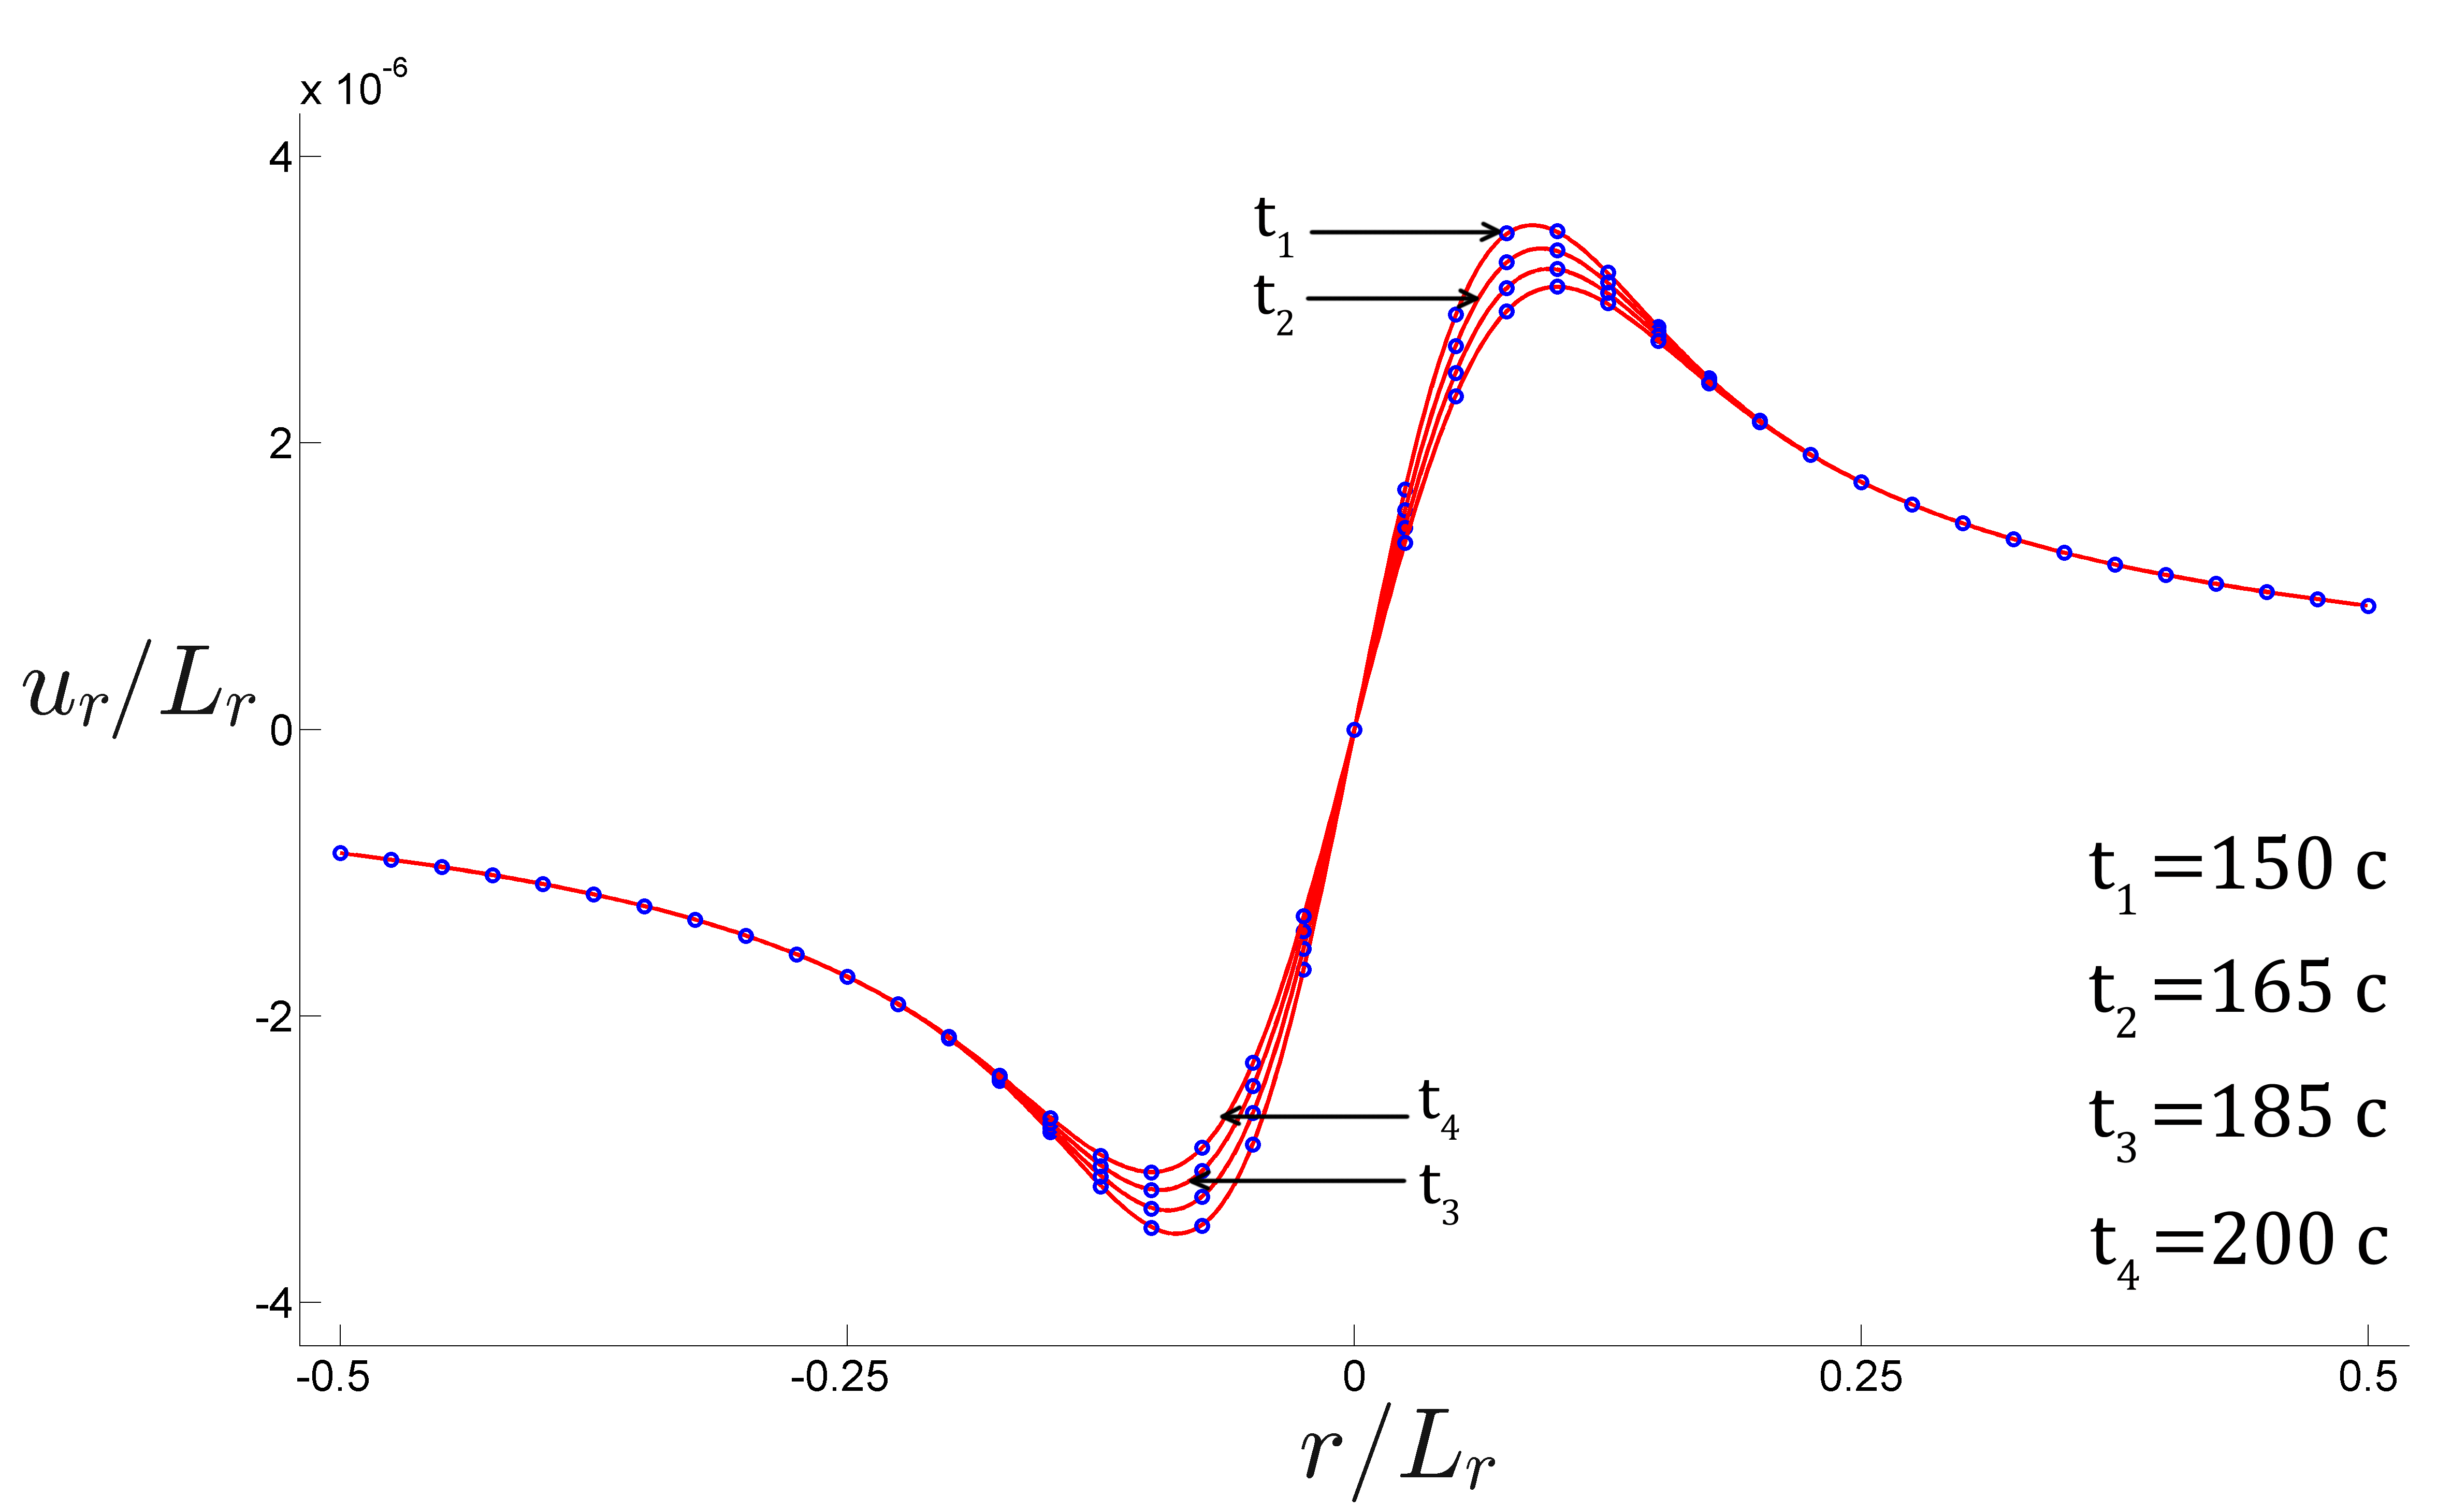
\includegraphics[width=0.88\textwidth]{figs/disp_line_mom2.png}
%   \caption{ Нормированное перемещение в различные моменты времени: красным
% цветом показано аналитическое решение, синим~--– результаты расчета }
%   \label{fig::disp_line_mom}
% \end{figure}

%\newpage

\subsection{Задача о постоянном линейном источнике}

На основе решения задачи о мгновенном линейном источнике в пороупругой среде
путем суперпозиции решений можно получить решение для линейного постоянного источника~\cite{wang_2000}:
%
\begin{equation}
\label{eq:constlinep}
p(r,t) = \frac{V_f}{4\pi (k/\mu)} E_1 \left(\frac{r^2}{4 c_f t}\right),
\end{equation}
%
\begin{multline}
\label{eq:constlinur}
u_r(r,t) = \frac{3b}{(3K+4\nu)(k/\mu)} \cdot \frac{V_f}{8 \pi} r \\ 
\cdot
\left\{ \frac{4 c_f t}{r^2}\left[1 - \exp{\left( -\frac{r^2}{4 c_f t}\right)} \right] + E_1 \left(\frac{r^2}{4 c_f t}\right) \right\},
\end{multline}
%
где
%
\begin{equation*}
E_1(u) = \int\limits_u^\infty \frac{\exp(-\xi)}{\xi} d\xi.
\end{equation*}

В данных выражениях $V_f$ имеет смысл объема жидкости, притекающего через источник в единицу времени.

Область, граничные условия и расчетная сетка брались аналогично таковым для задачи
о мгновенном линейном источнике. Объем притока в единицу времени задавался как $V_f = 1 \text{м}^3 / \text{с}$.
Расчет начинался с момента времени $t_{\text{start}}=1000$ c, проводился с шагом $\Delta t = 100$ c до времени $t_{\text{end}}=1800$ c.



Результаты расчетов приведены на
рис.~\ref{fig::press_const_line_source},
% и~\ref{fig::disp_const_line_source},
где показано распределение нормированного давления и перемещения в начальный и конечный моменты времени.
Как видно из рисунков, получено приемлемое совпадение с аналитическими результатами. Различия связаны с невозможностью
разрешить сингулярность от источника с помощью используемых в программном комплексе методов.

\begin{figure}[t!]
\centering
  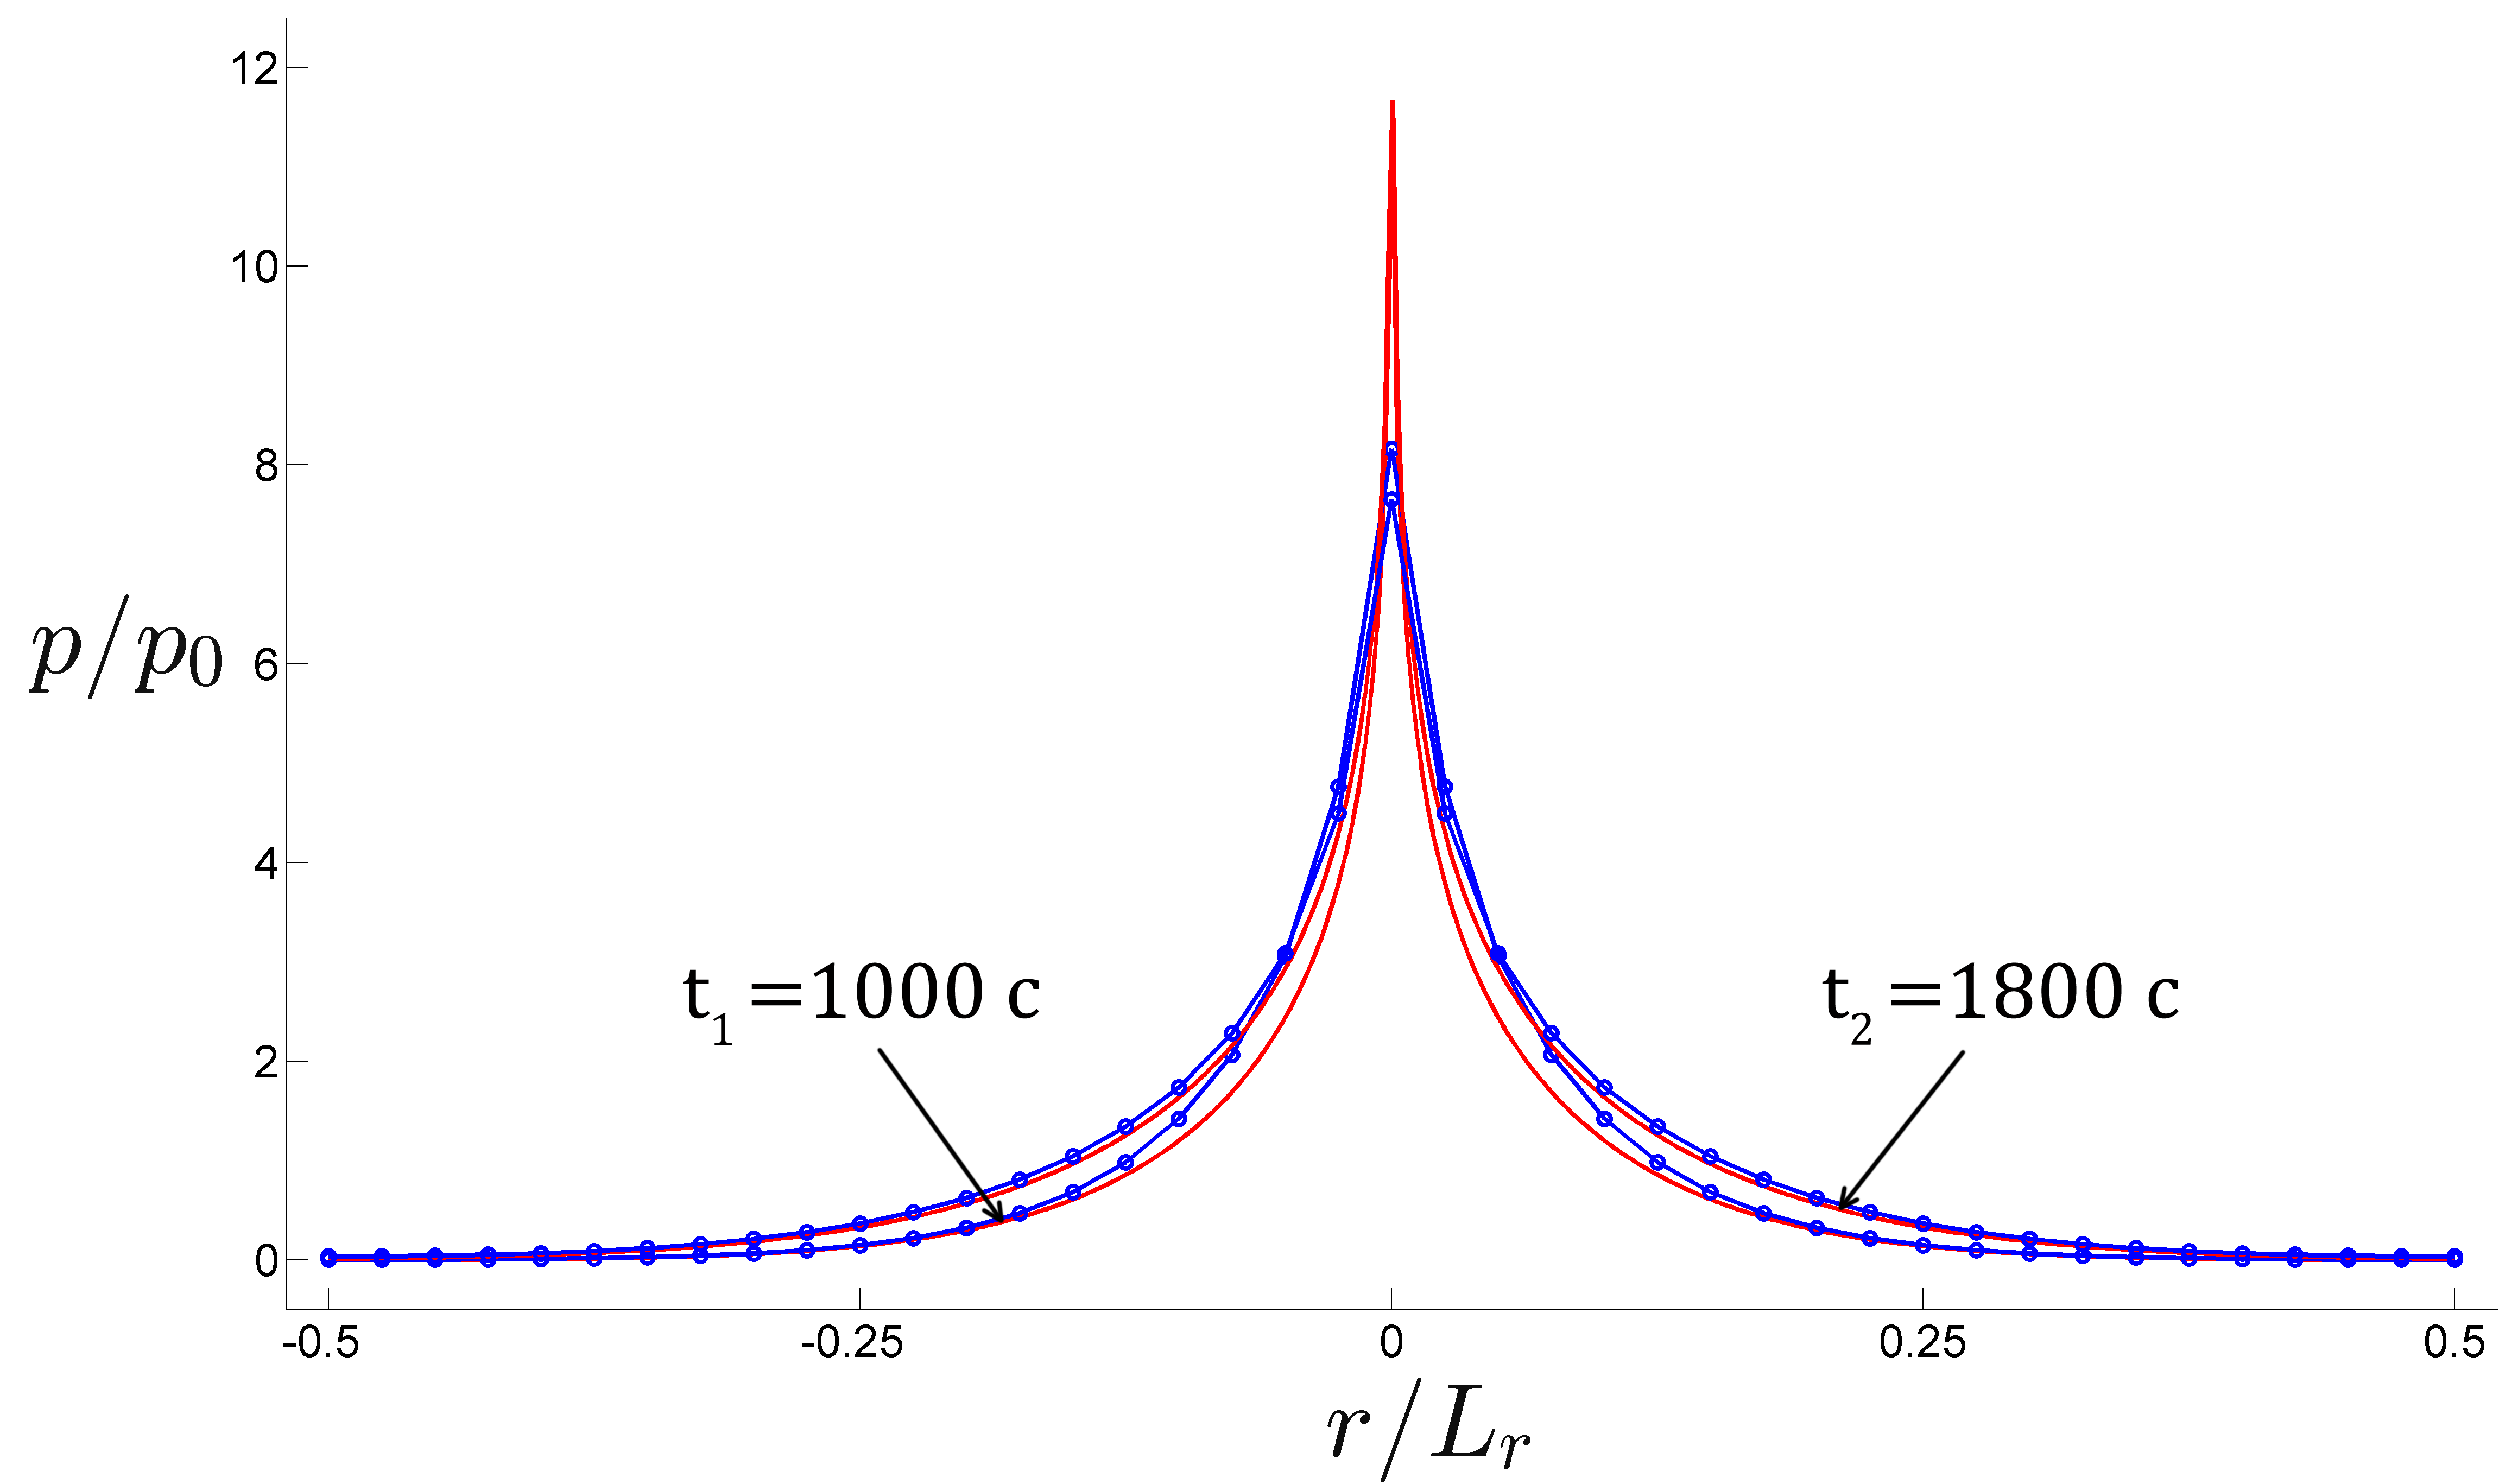
\includegraphics[width=0.8\textwidth]{figs/press_const_line_source2.png}\\
  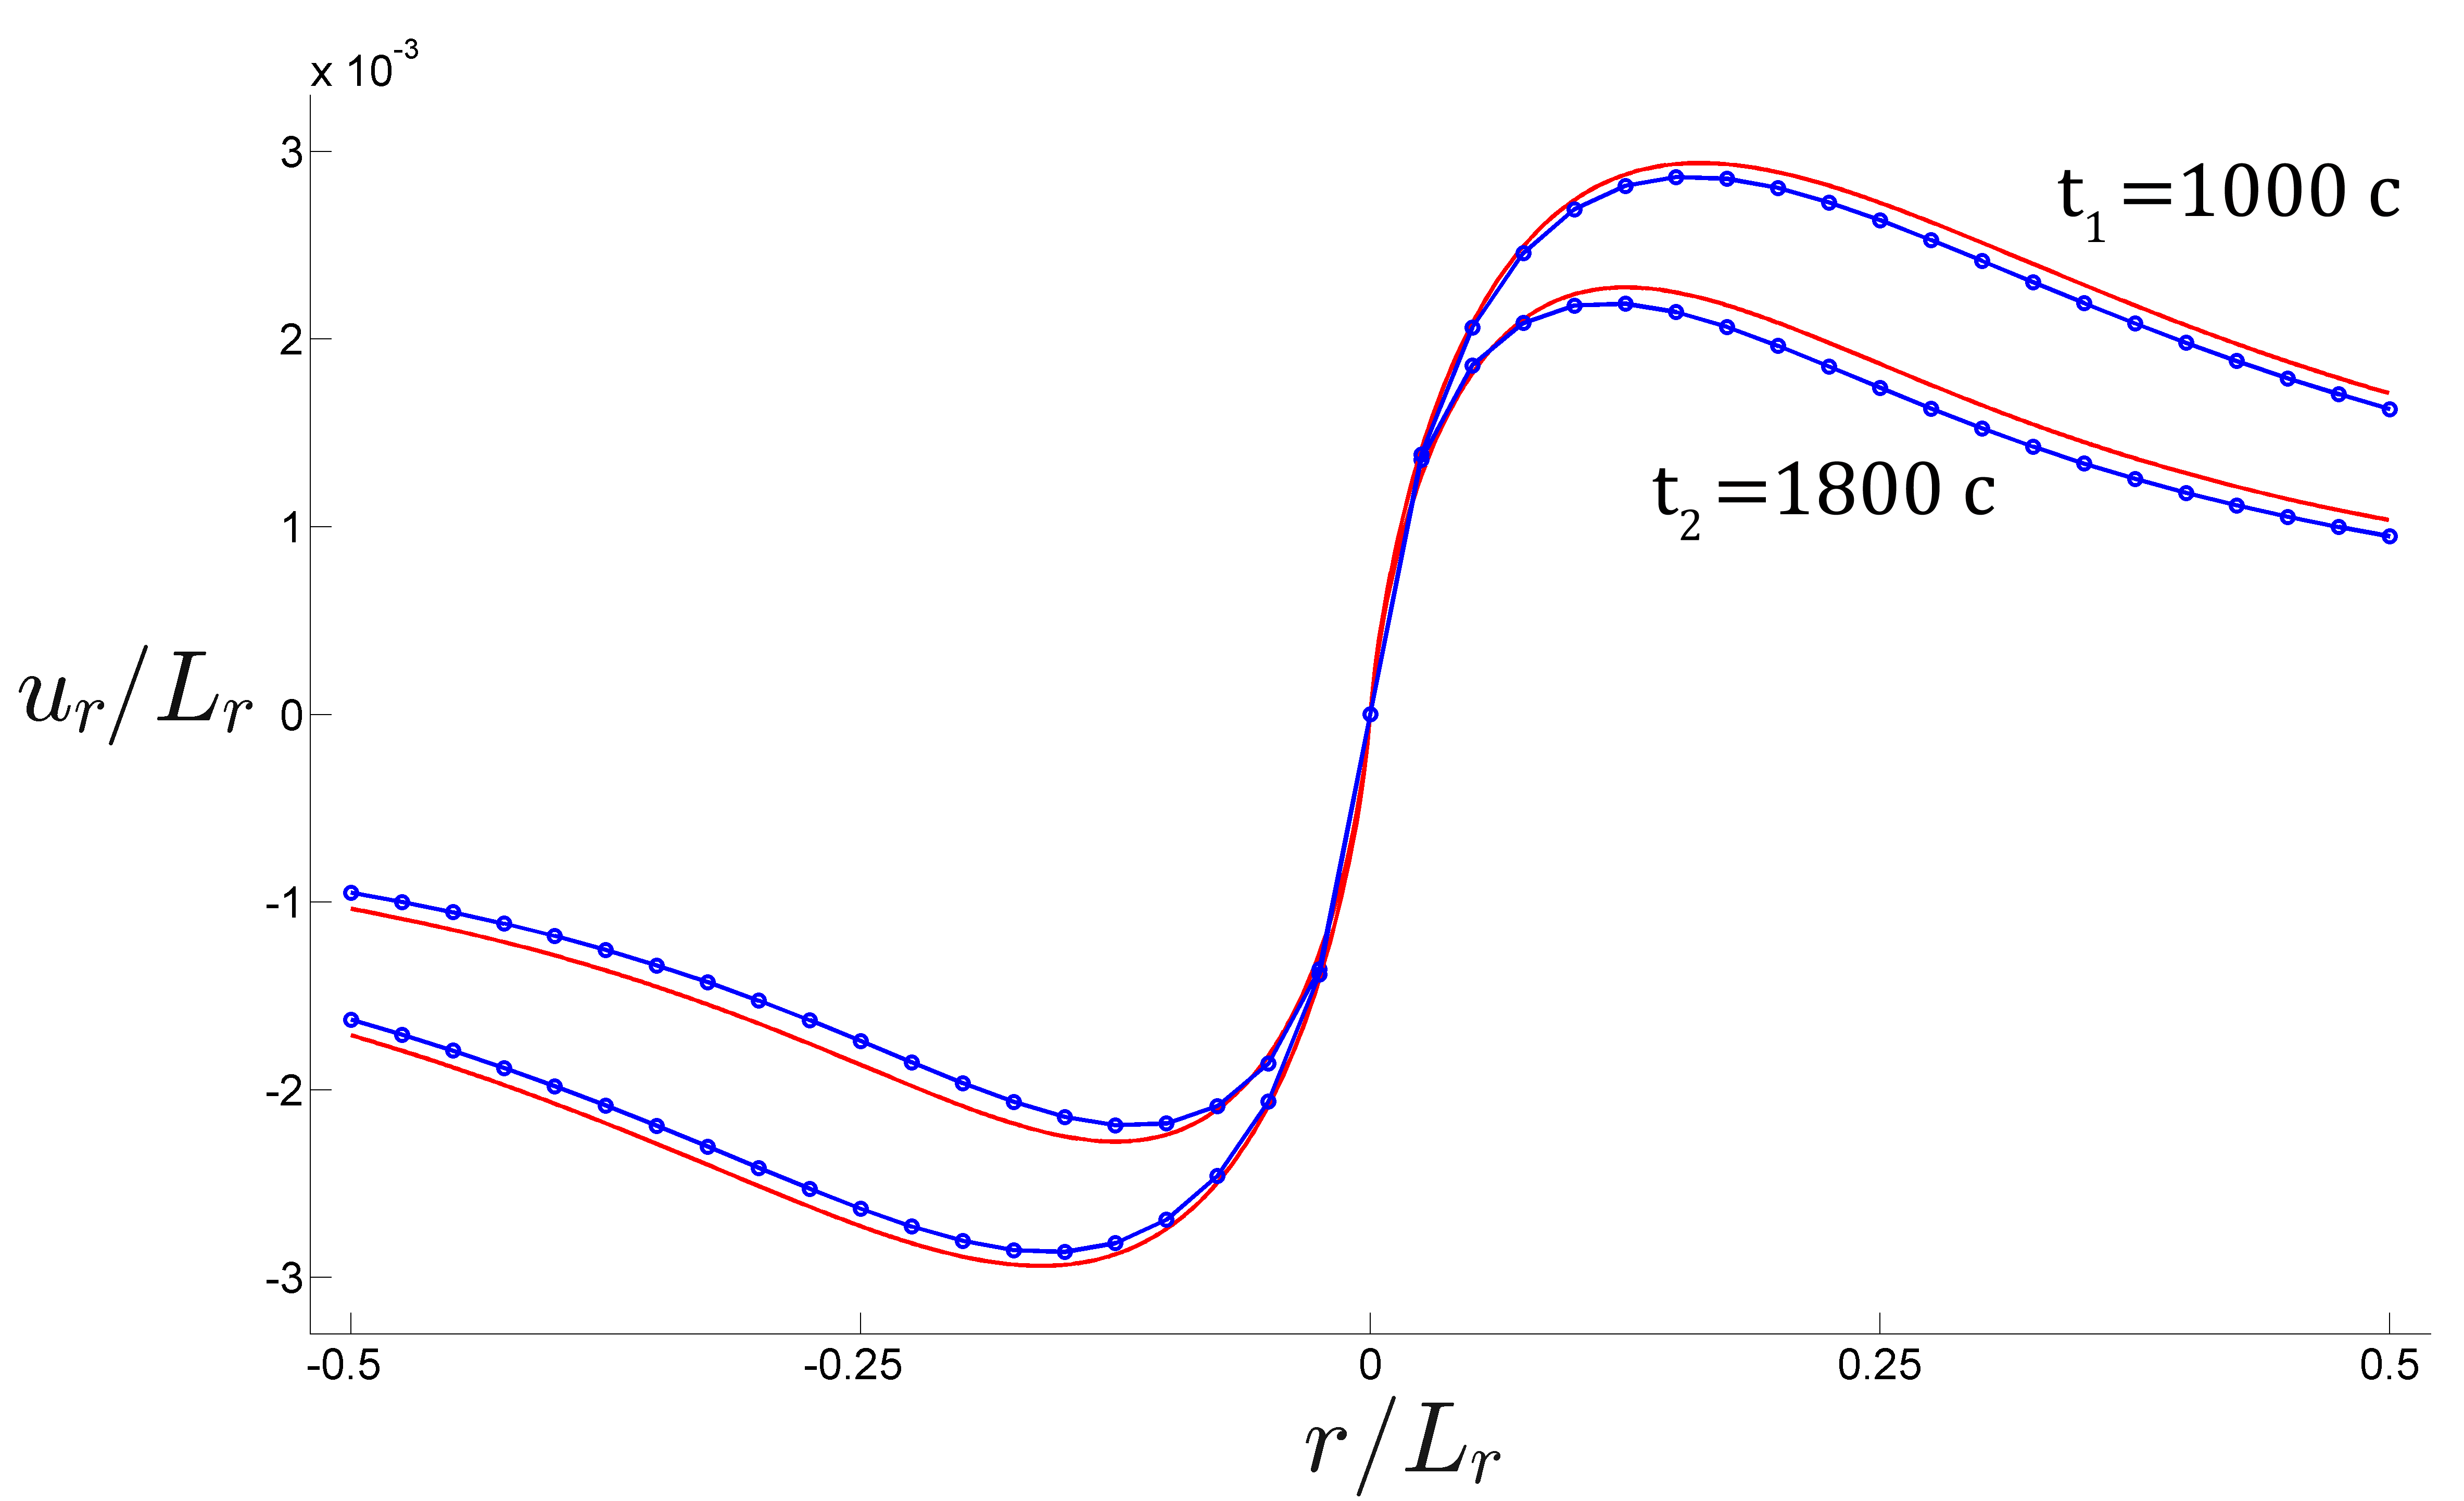
\includegraphics[width=0.8\textwidth]{figs/disp_const_line_source2.png}
  \caption{ Задача о постоянном линейном источнике. Нормированное давление (вверху) и перемещение (внизу) в различные моменты времени: красным
цветом показано аналитическое решение, синим~--– результаты расчета.}
  \label{fig::press_const_line_source}
\end{figure}

% \begin{figure}[h!]
% \centering
%   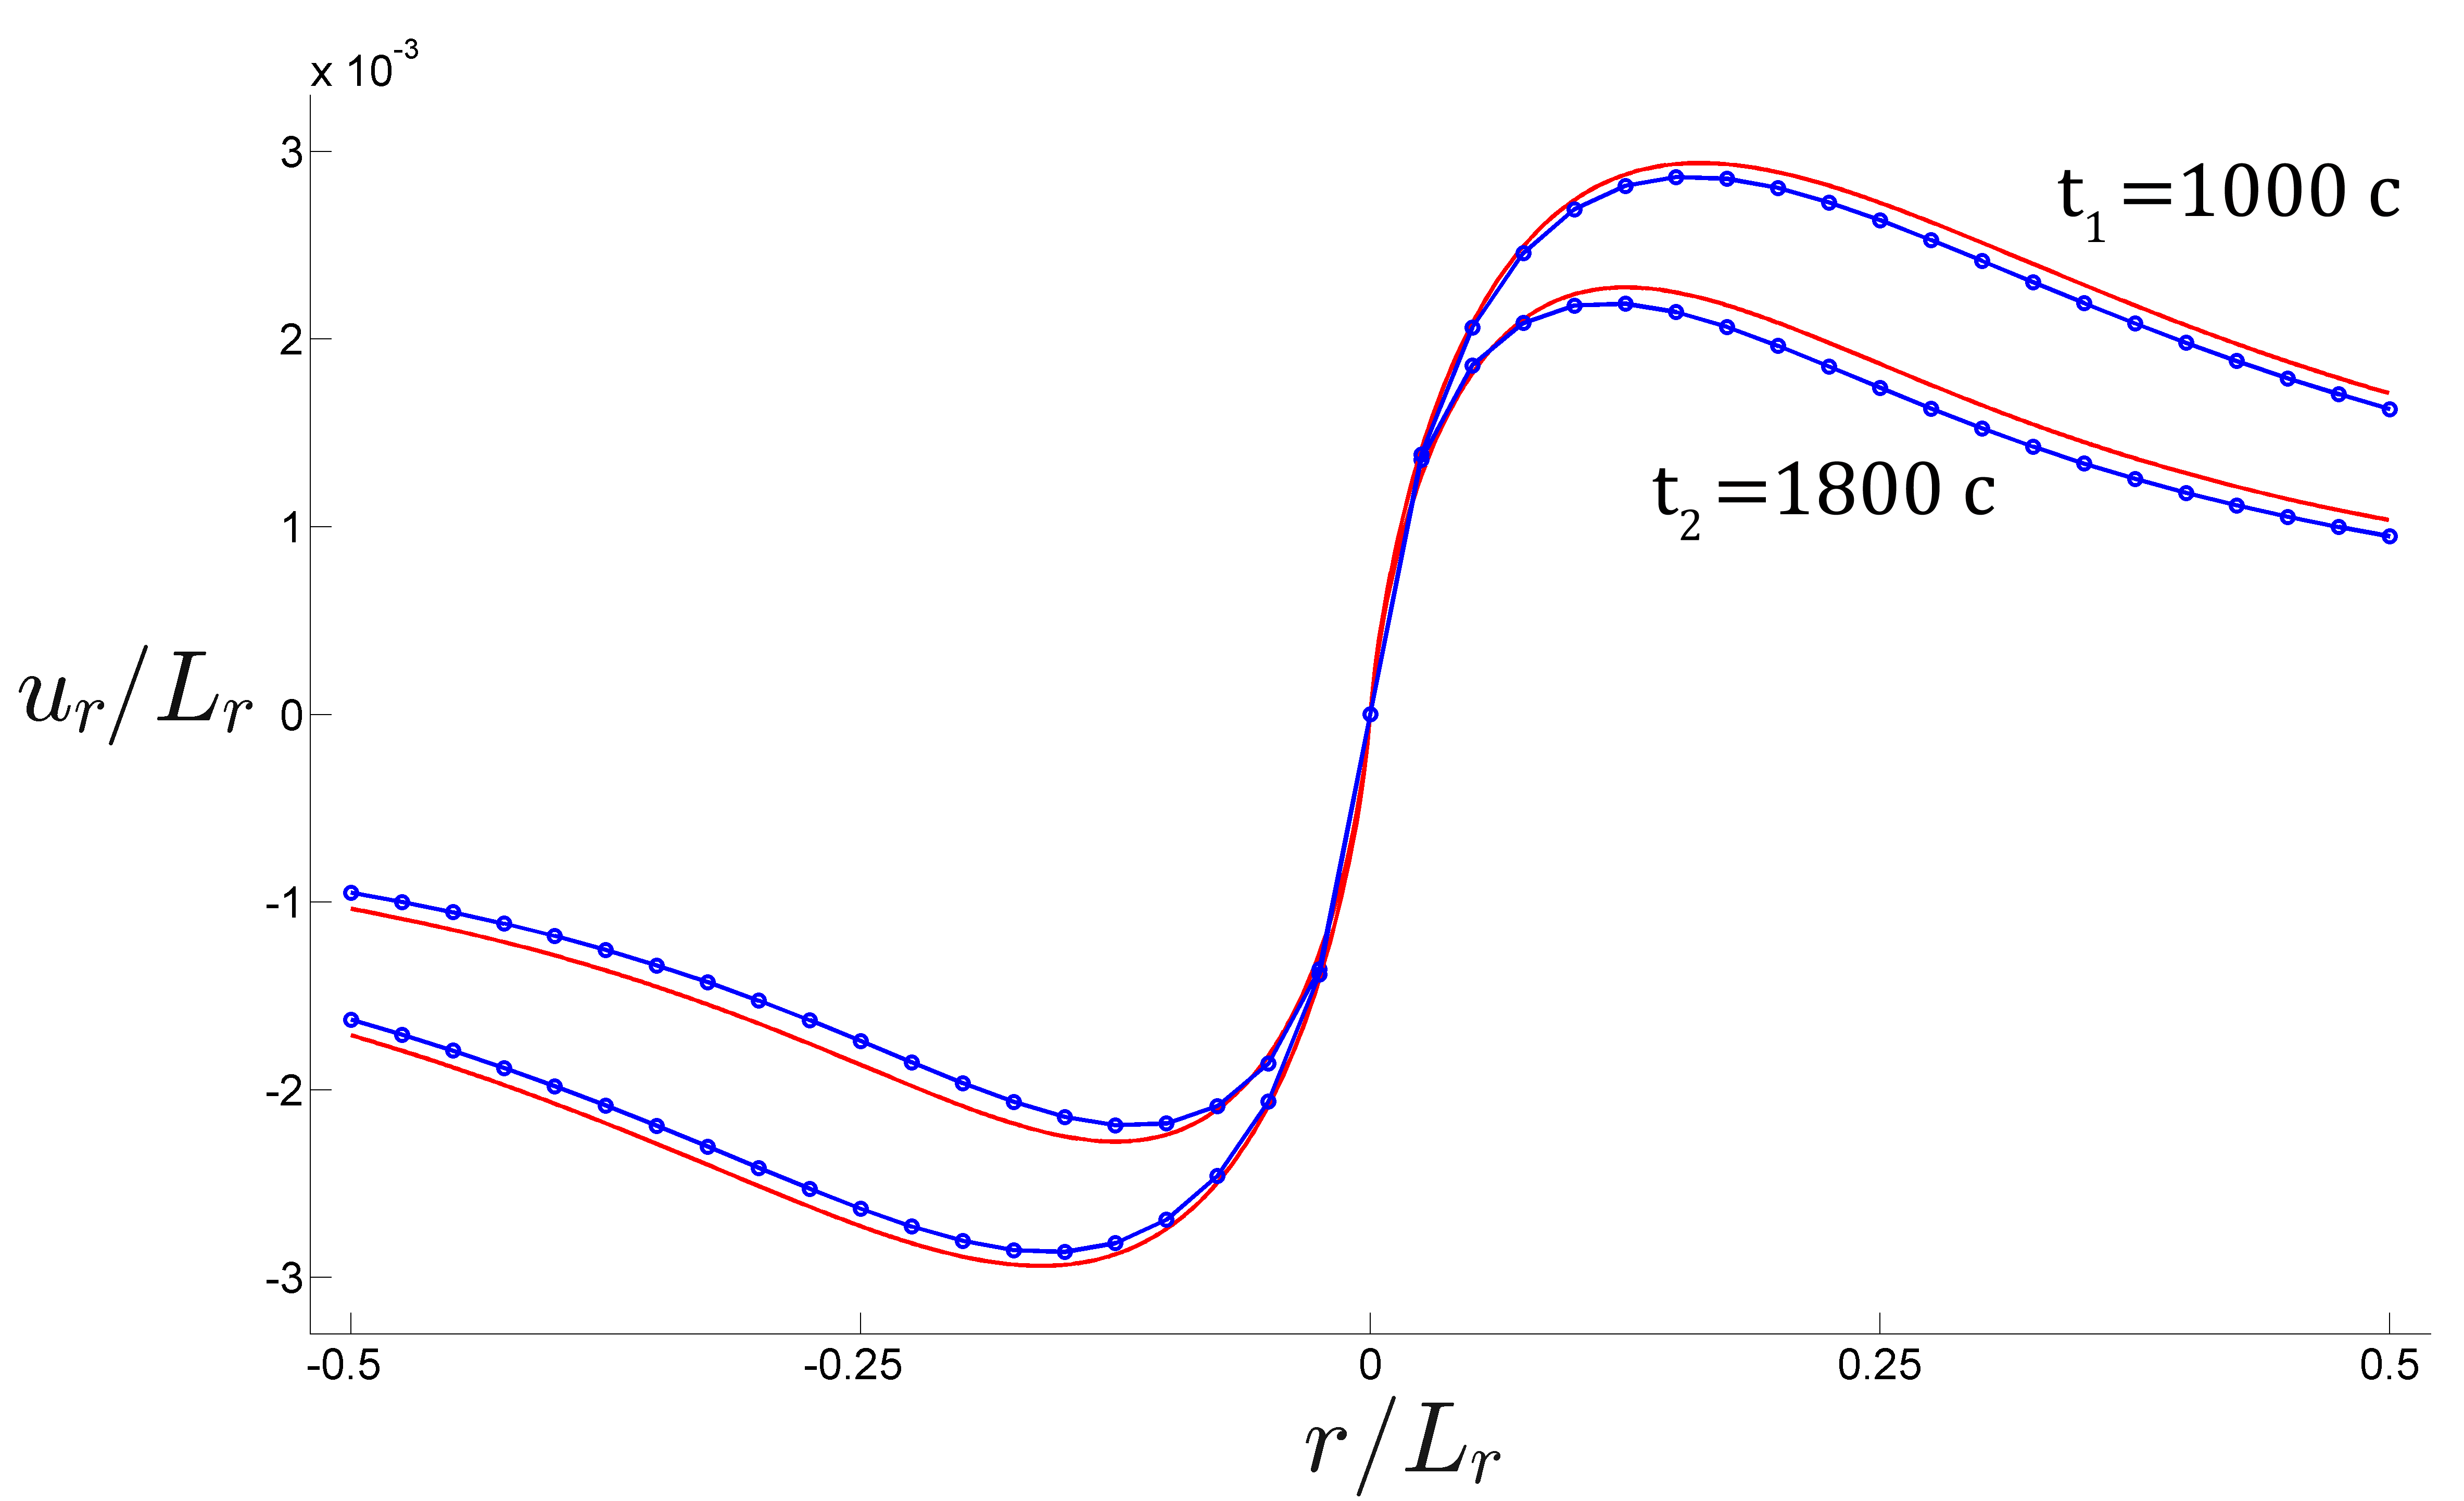
\includegraphics[width=0.98\textwidth]{figs/disp_const_line_source2.png}
%   \caption{ Нормированное перемещение в различные моменты времени: красным
% цветом показано аналитическое решение, синим – результаты расчета}
%   \label{fig::disp_const_line_source}
% \end{figure}

%\newpage
\subsection{Задача консолидации Терцаги}

Одной из классических задач пороупругости, для которых
известно аналитическое решение, является классическая одномерная задача консолидации Терцаги~\cite{terzaghi_1996}.

Рассмотрим насыщенную пороупругую область с линейными размерами $L_x$,
$L_y$, $L_z$. Верхняя граница резервуара имеет координату $z=0$,
нижняя~-- $z = L_z$.  Нижняя и боковые границы являются
непротекаемыми, при этом нижняя стенка закреплена, а боковые стенки
могут деформироваться только в вертикальном направлении. Верхняя
граница является проницаемой, к ней прикладывается сжимающее
напряжение величиной $T_z = -\sigma_0$, что приводит к деформации
пороупругой среды. В такой постановке задача является одномерной,
решение решение не зависит от $x$ и $y$.  Схематично постановка задачи
представлена на рис.~\ref{fig:terzaghi}.

%
\begin{figure}[h!]
\centering
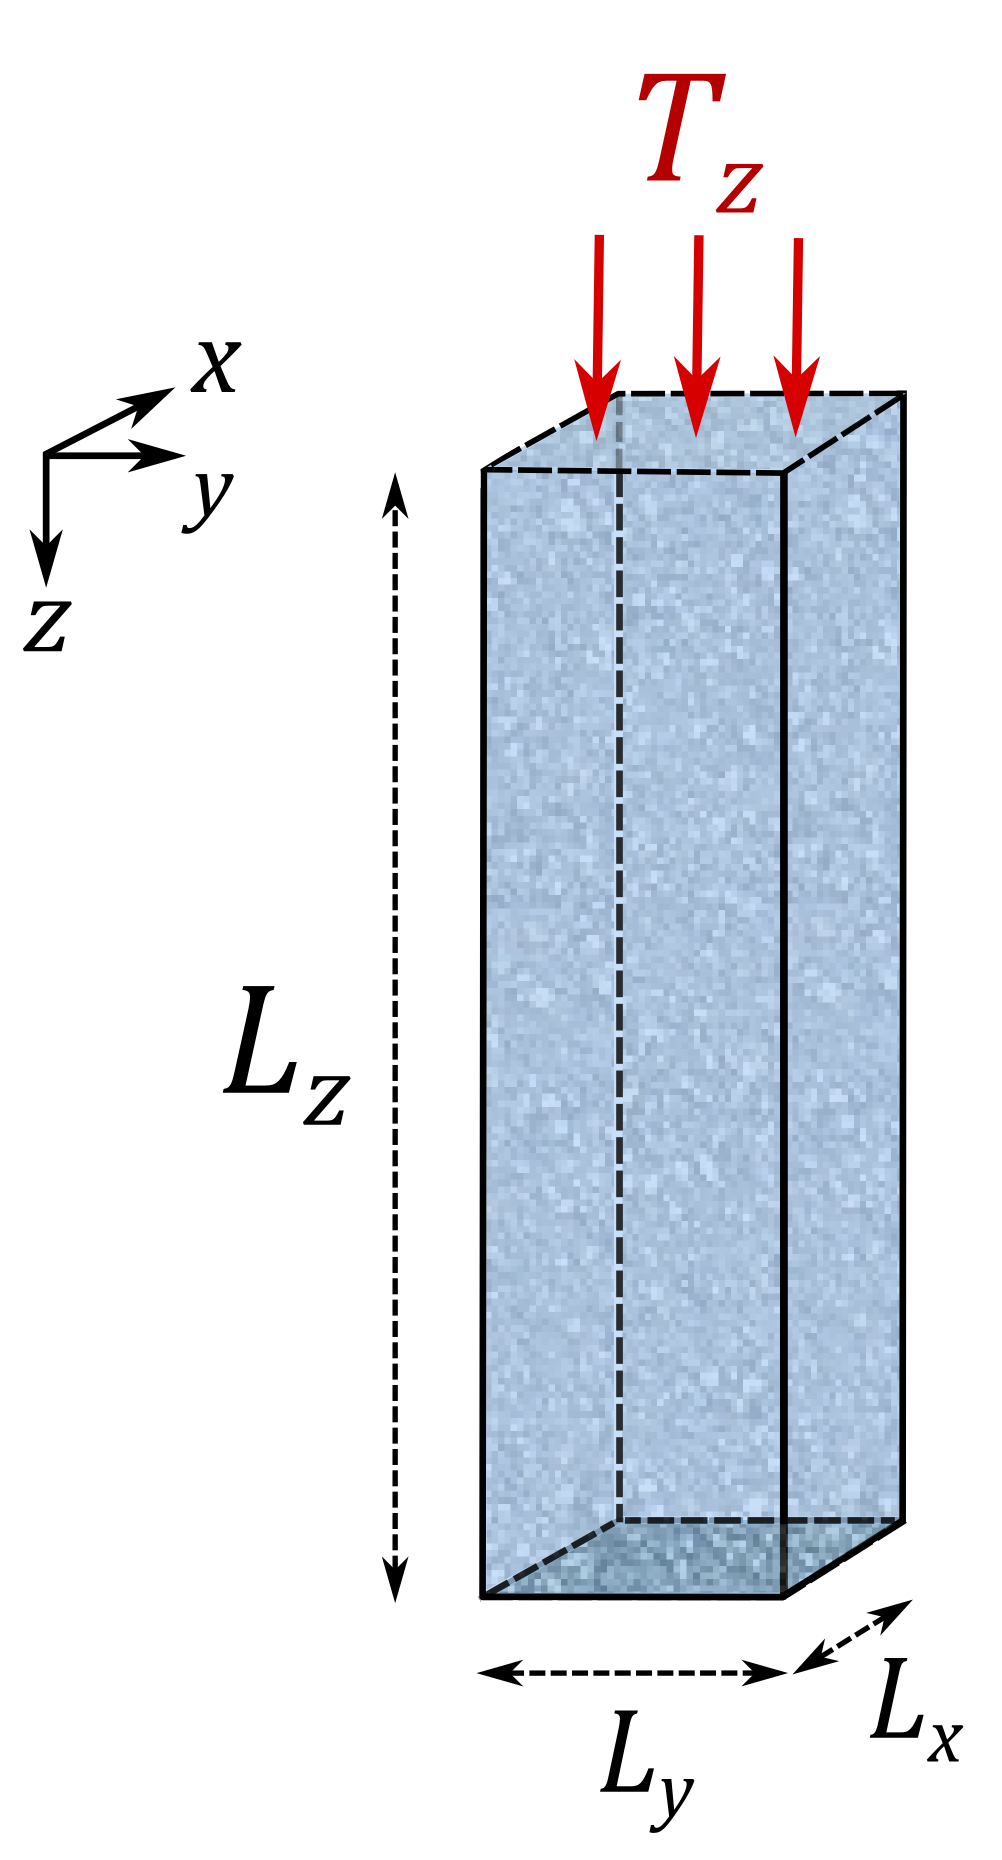
\includegraphics[width=0.35\textwidth]{./figs/terzaghi.png}
\caption{Схематичный вид задачи Терцаги.}\label{fig:terzaghi}
\end{figure}
% 

Граничные условия в одномерной постановке ставятся следующим образом:
%
\begin{equation}
\begin{aligned}
\label{eq:bcTer}
%
& z = 0:   & &\sigma_{zz}(0,t) = -\sigma_0, & &p(0,t) = 0, \\
%
& z = L_z: & &u_z(L_z,t) = 0, & &\cfrac{\partial p}{\partial z} = 0.
%
\end{aligned}
\end{equation}
%

Начальные условия после мгновенного нагружения задаются в виде
%
\begin{equation}
%\begin{split}
\label{eq:icTer}
%
u_z(z,0^+) \equiv u_0 = \sigma_0 (L_z - z) / K_v^{(u)},\quad
p(z,0^+) \equiv p_0 = \gamma \sigma_0.
%
%\end{split}
\end{equation}

Аналитическое решение задачи может быть записано как~\cite{wang_2000}:
%%
\begin{multline}
\label{eq:Pter}
%
p(z,t) = p_0 - p_0 \sum \limits_{m=0}^{\infty} \left(-1\right)^m
%
\left[   
\text{erfc} \cfrac{(2m+1)L_z - (z-L_z)}{\sqrt{4ct}} \right. \\ \left. + \; \text{erfc} \cfrac{(2m+1)L_z+(z-L_z)}{\sqrt{4ct}}
\right],
%
\end{multline}
%%

%%
\begin{multline}
\label{eq:Uter}
%
u_z(z,t)= u_0 + c_m\gamma\sigma_0 
%
\left[
(L_z-z) - \cfrac{8L_z}{\pi^2} \sum \limits_{m=0}^{\infty} \cfrac{1}{(2m+1)^2} \right. \\
\left. \cdot \exp \left( \cfrac{-(2m+1)^2\pi^2 c t}{4L_z^2}  \right) 
\cdot \cos \left( \cfrac{(2m+1)\pi z}{2 L_z}  \right)
\right].
%
\end{multline}
%%

Здесь
%
\begin{gather*}
%
\gamma = \cfrac{B(1+\nu_u)}{3(1-\nu_u)}, \quad
c_m\gamma = \cfrac{\nu_u-\nu}{2G(1-\nu)(1-\nu_u)}, \\[7pt]
%
c = \cfrac{2kG(1-\nu)(\nu_u-\nu)}{\mu b^2 (1-2\nu)^2(1-\nu_u)}, \quad K_v^{(u)} = \cfrac{2G(1-\nu_u)}{1-2\nu_u}.
%
\end{gather*}
%

В качестве данных для сравнения используются нормированные значения $\overline{p}$ и
$\overline{u}_z$:
%
\begin{equation*}
%
\overline{p} = \cfrac{p}{p_0}, \quad \overline{u} = \cfrac{u_z}{L_z}, \quad 
\overline{z} = \cfrac{z}{L_z}, \quad \overline{\tau} = \cfrac{ct}{L_z^2}.
%
\end{equation*}
%
%\vspace{5mm}

Конкретные значения используемых для расчетов параметров приведены в табл.~\ref{tab:terzaghi}.
%
%%
\begin{table}[h!]
\centering
%
\renewcommand{\arraystretch}{1.5}
\renewcommand{\tabcolsep}{6 pt} 
\begin{tabular}{|c|c|c|c|c|c|c|}
\hline
$L_z$ & $L_x$ & $L_y$ & $\sigma_0$ & $t_{\text{start}}$ & $t_{\text{end}}$ & $\Delta t$\\
\hline
 $15.0$ м & $1.0$ м & $1.0$ м & $1.0$ КПа & $0.0$ с & $1500.0$ с & $1.0$ с\\
\hline
\end{tabular}
%
\caption{Параметры для численного расчета задачи Терцаги.}\label{tab:terzaghi}
\end{table}
%%
%

Для численных расчетов использовалась тетраэдральная сетка, состоящая из 
$N_{nodes} = 1600$ узлов и $N_{elems} = 5346$ прямоугольных тетраэдров со сторонами
$h_x = h_y = 0.3333$ м, $h_z = 0.1515$ м. В отличие от представленной выше постановки задачи и аналитического решения
для нее при проведении расчетов в программном комплексе начало координат и ориентация оси $Oz$ были выбраны другими.
В силу этого при сравнении с аналитическим решением полученное численное решение при необходимости нормировалось соответствующим образом.

%
\begin{figure}[t!]
\centering
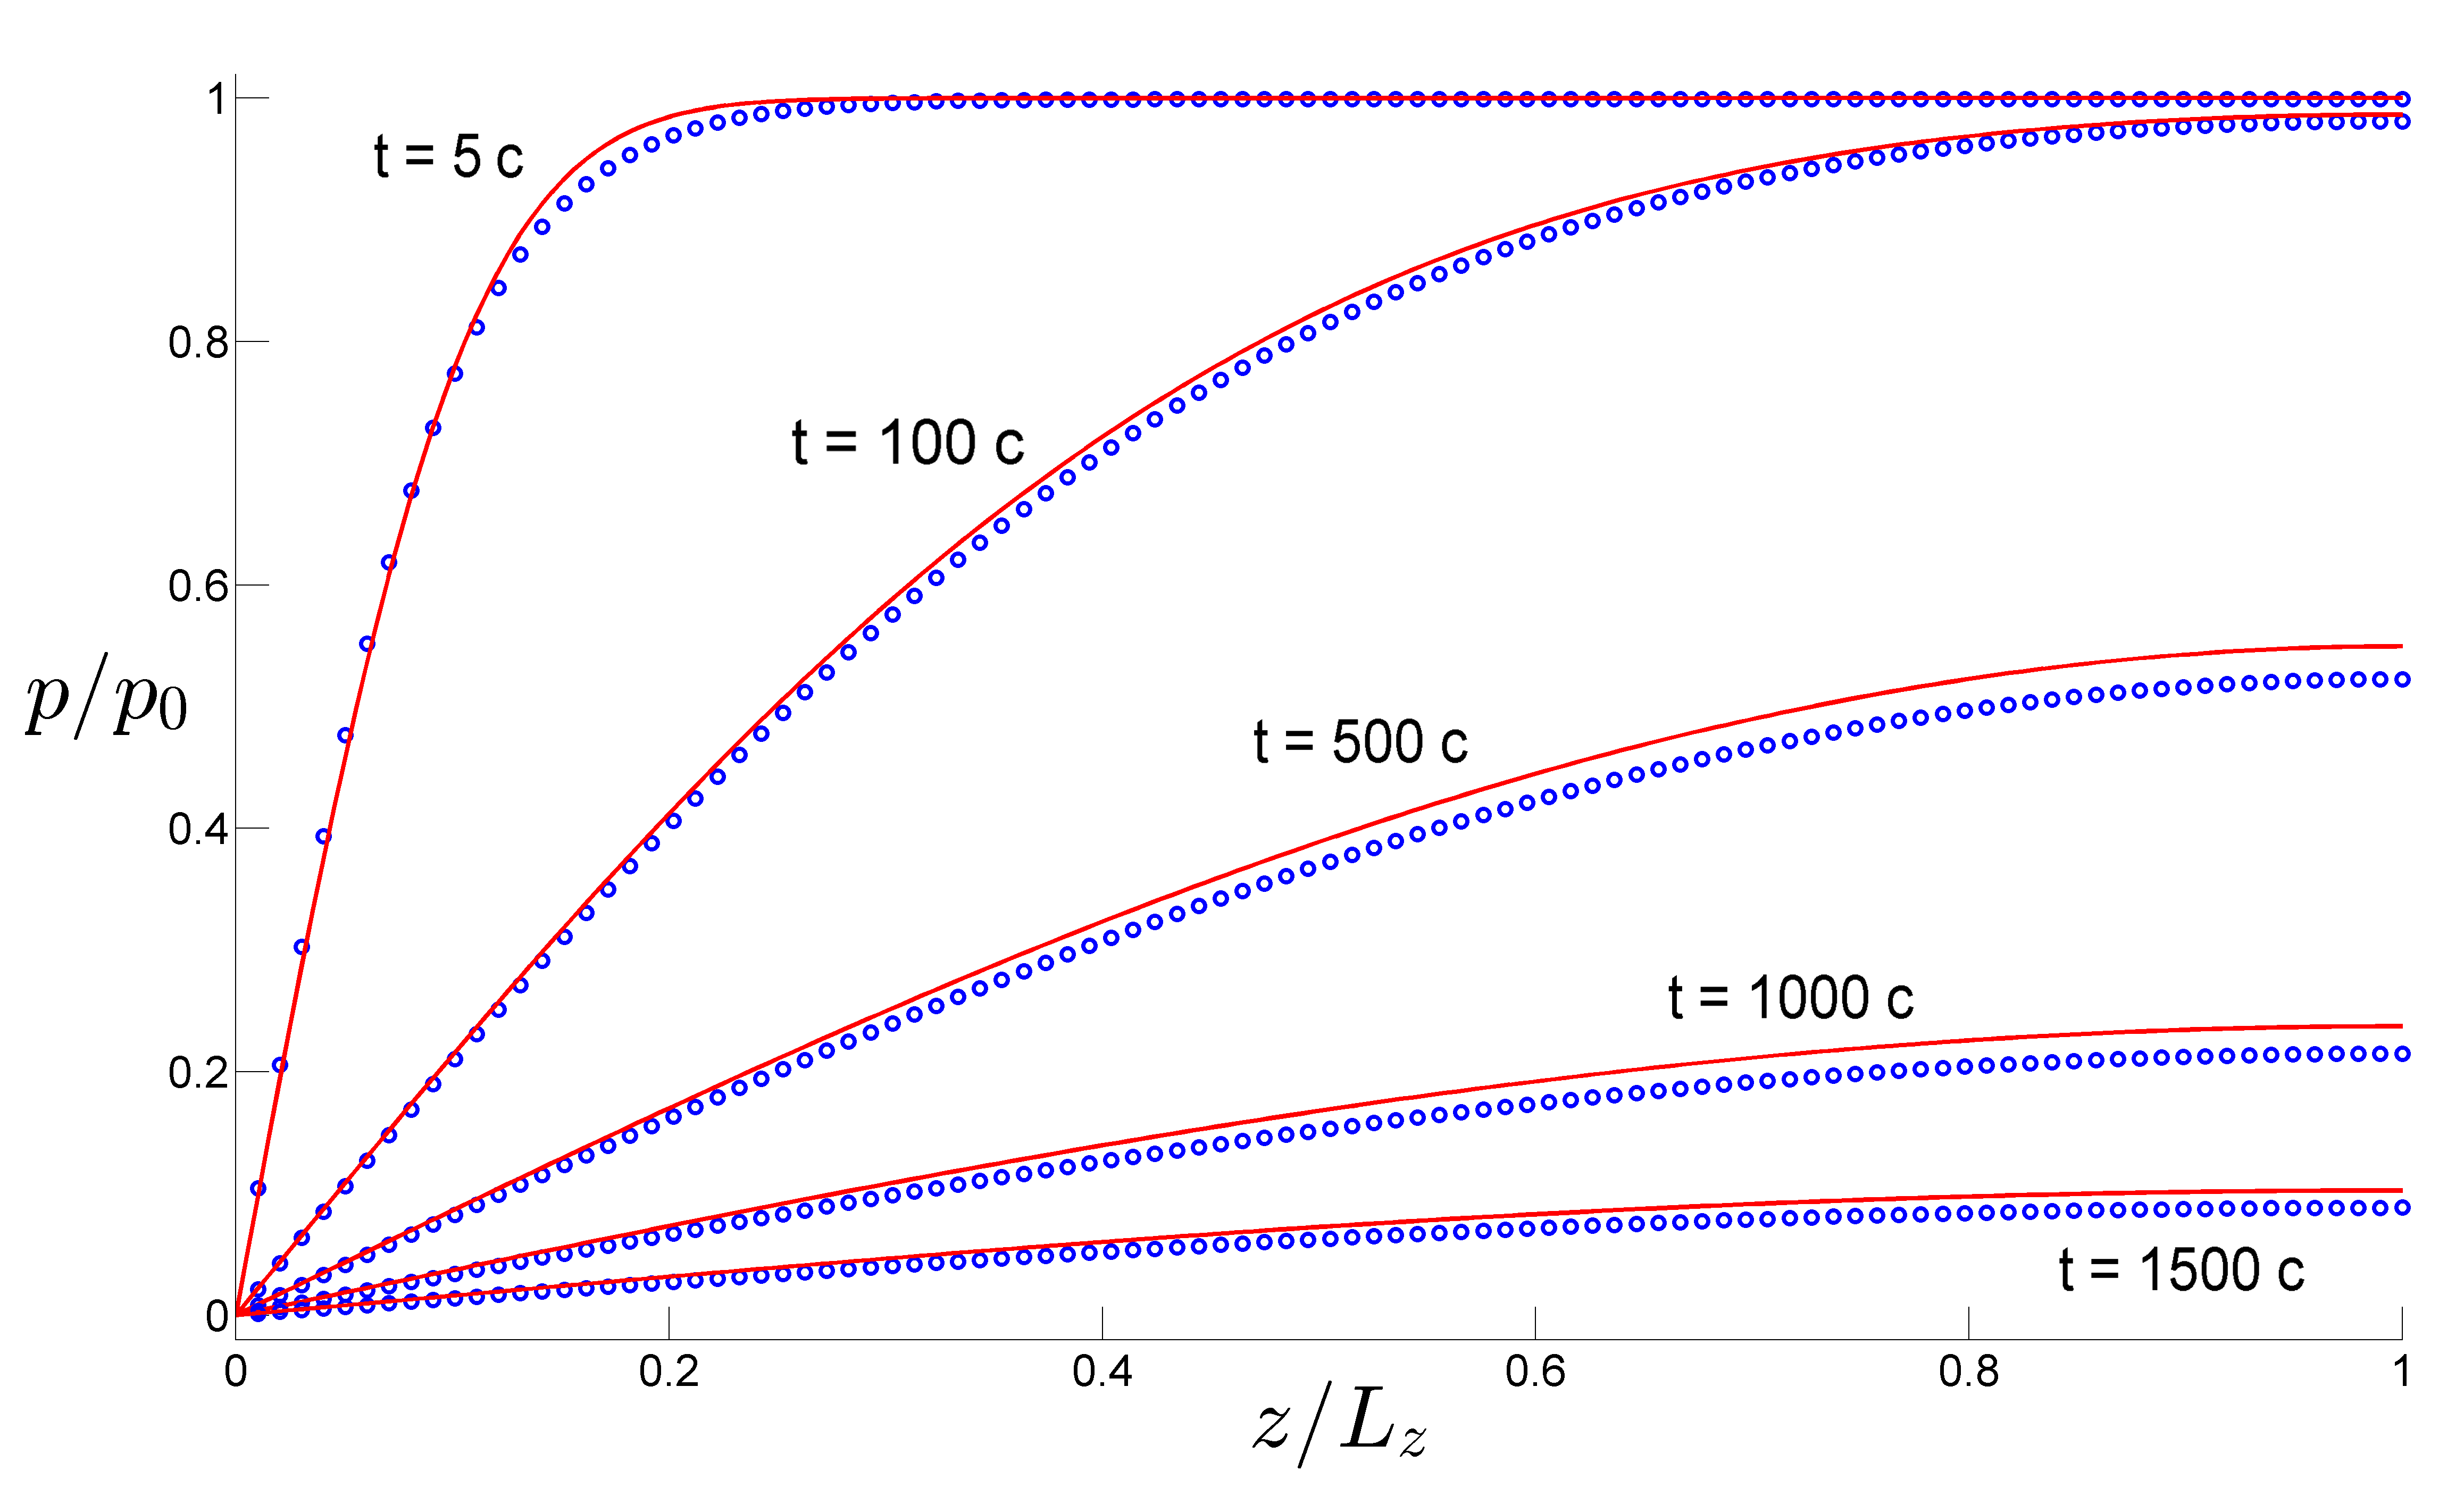
\includegraphics[width=0.9\textwidth]{./figs/pp0Ter.png}\\
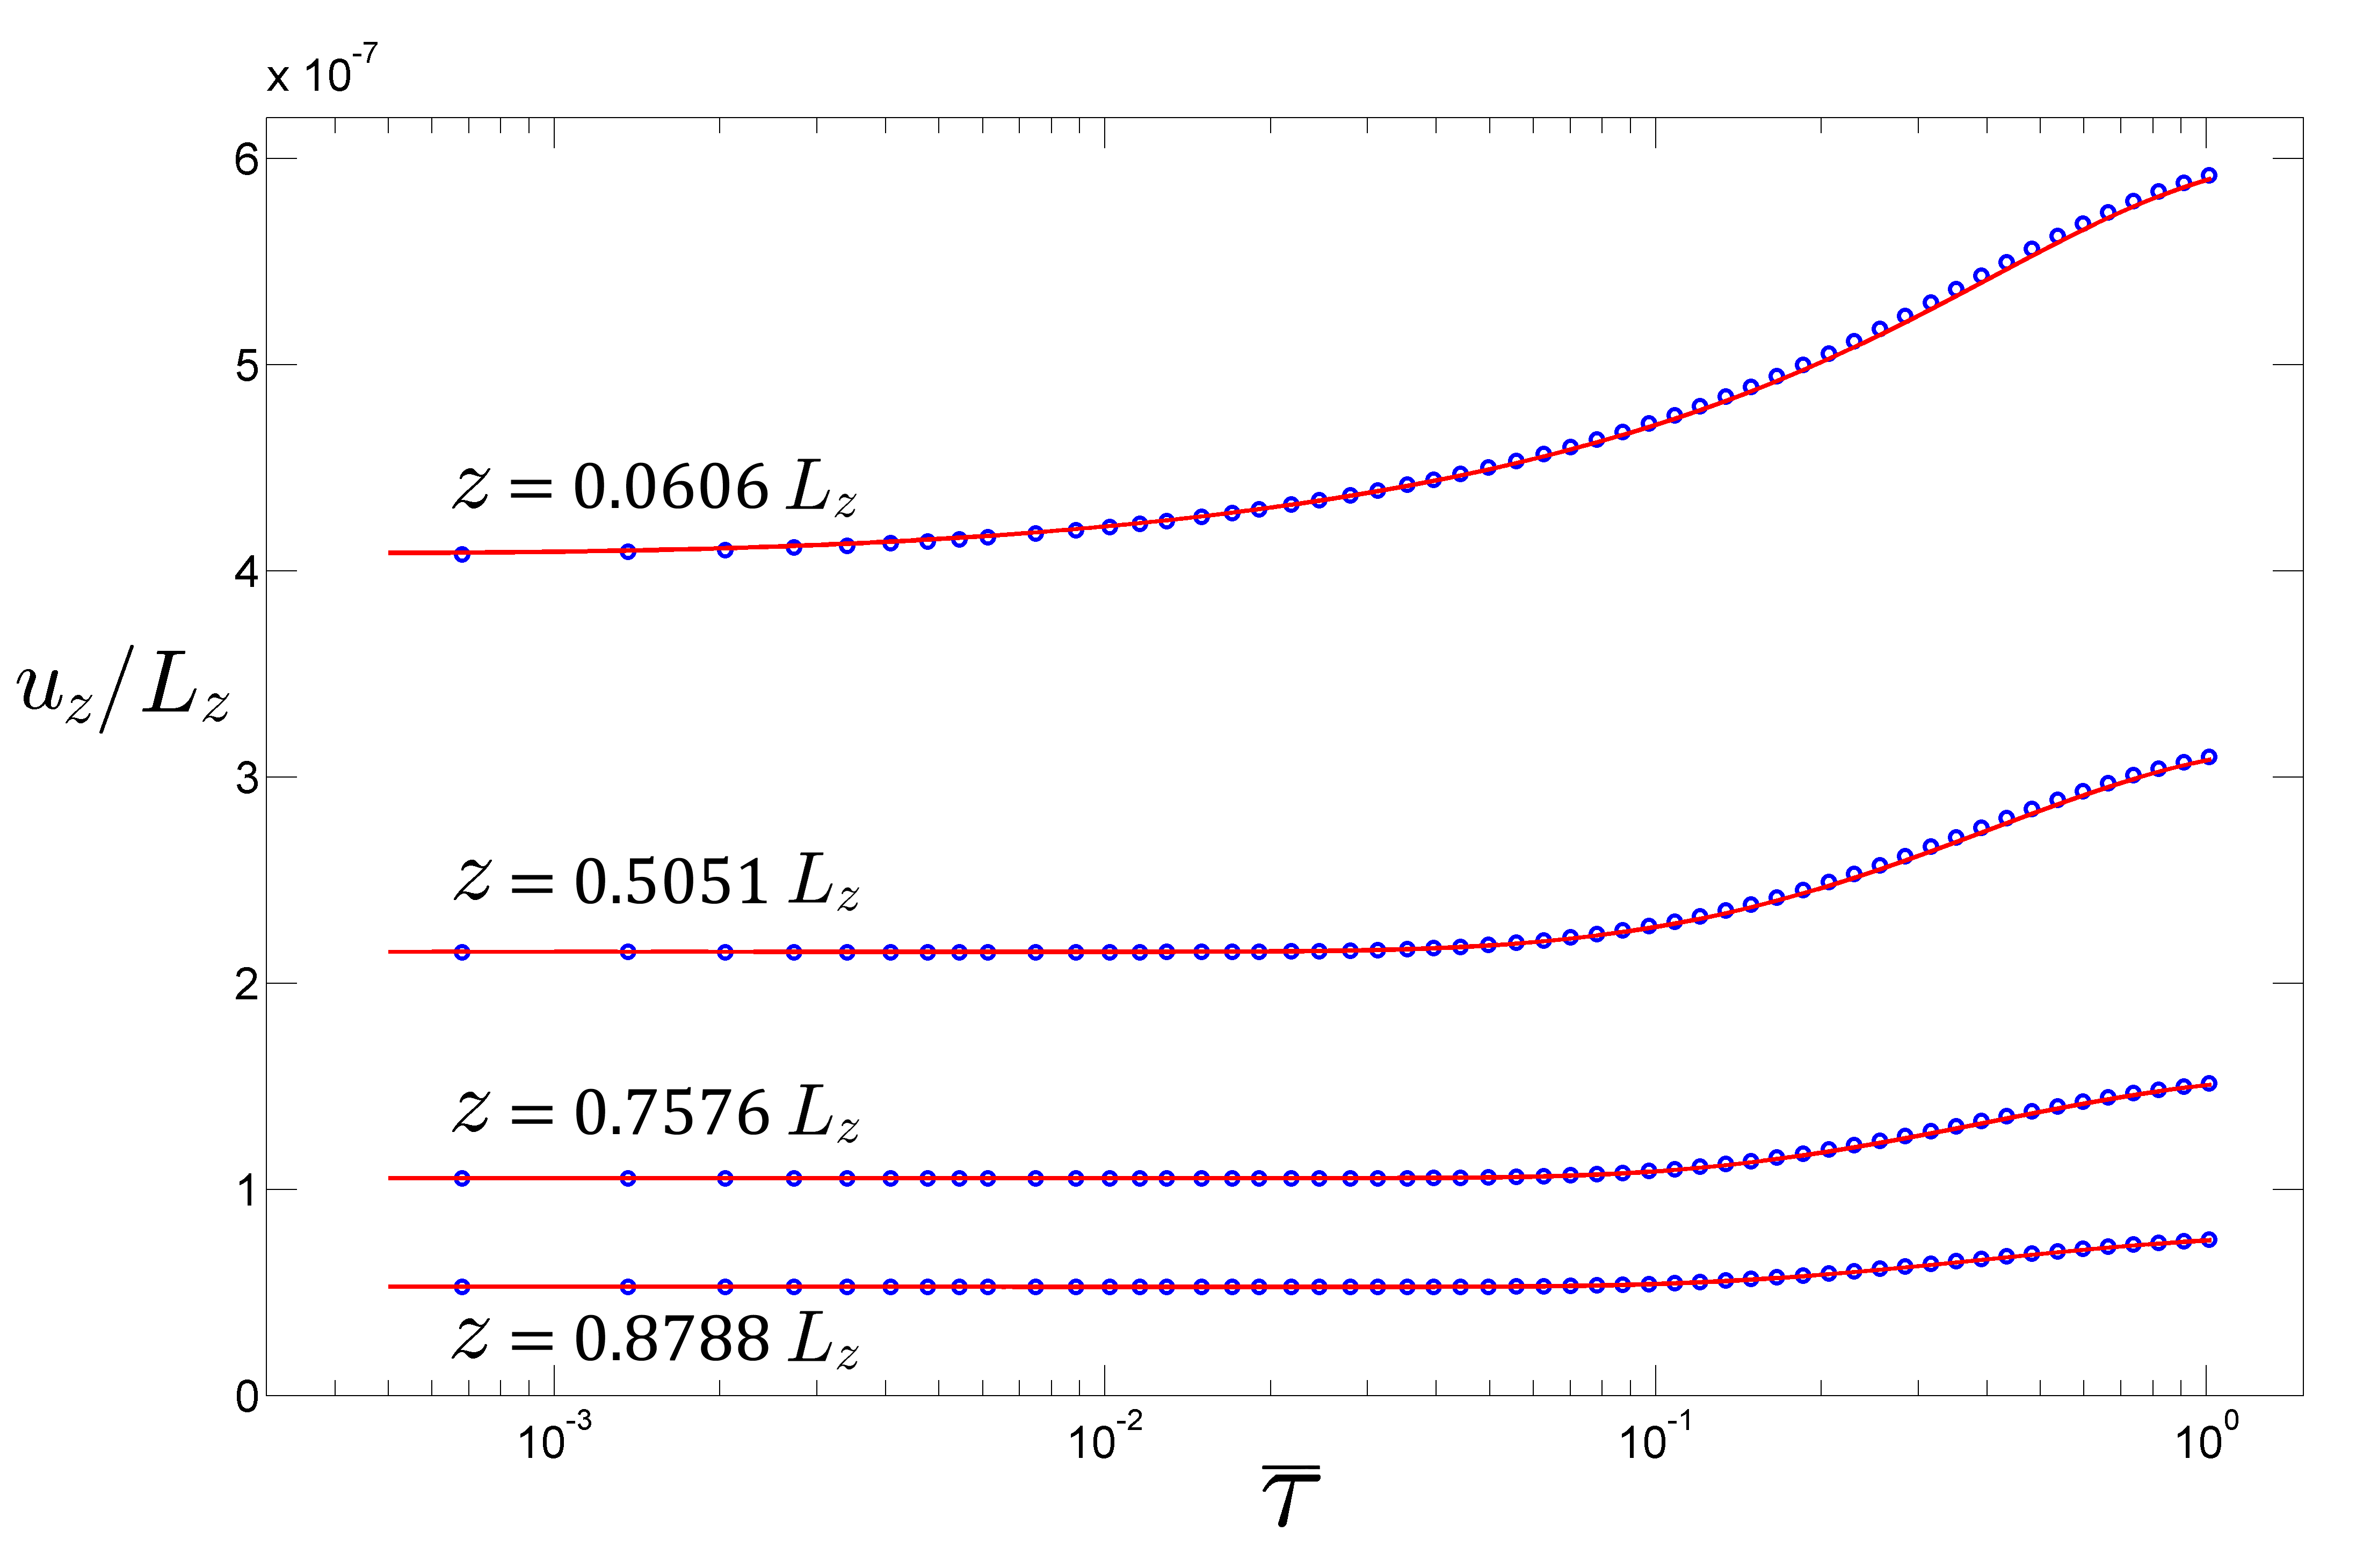
\includegraphics[width=0.9\textwidth]{./figs/uu0Ter.png}
\caption{ Задача консодидации Терцаги. Нормированное давление (вверху) и перемещение (внизу) в
  различные моменты времени: красным цветом показано
аналитическое решение, синим~--- результаты расчета.}\label{fig:terp}
\end{figure}
% 
% \begin{figure}[h!]
% \centering
% 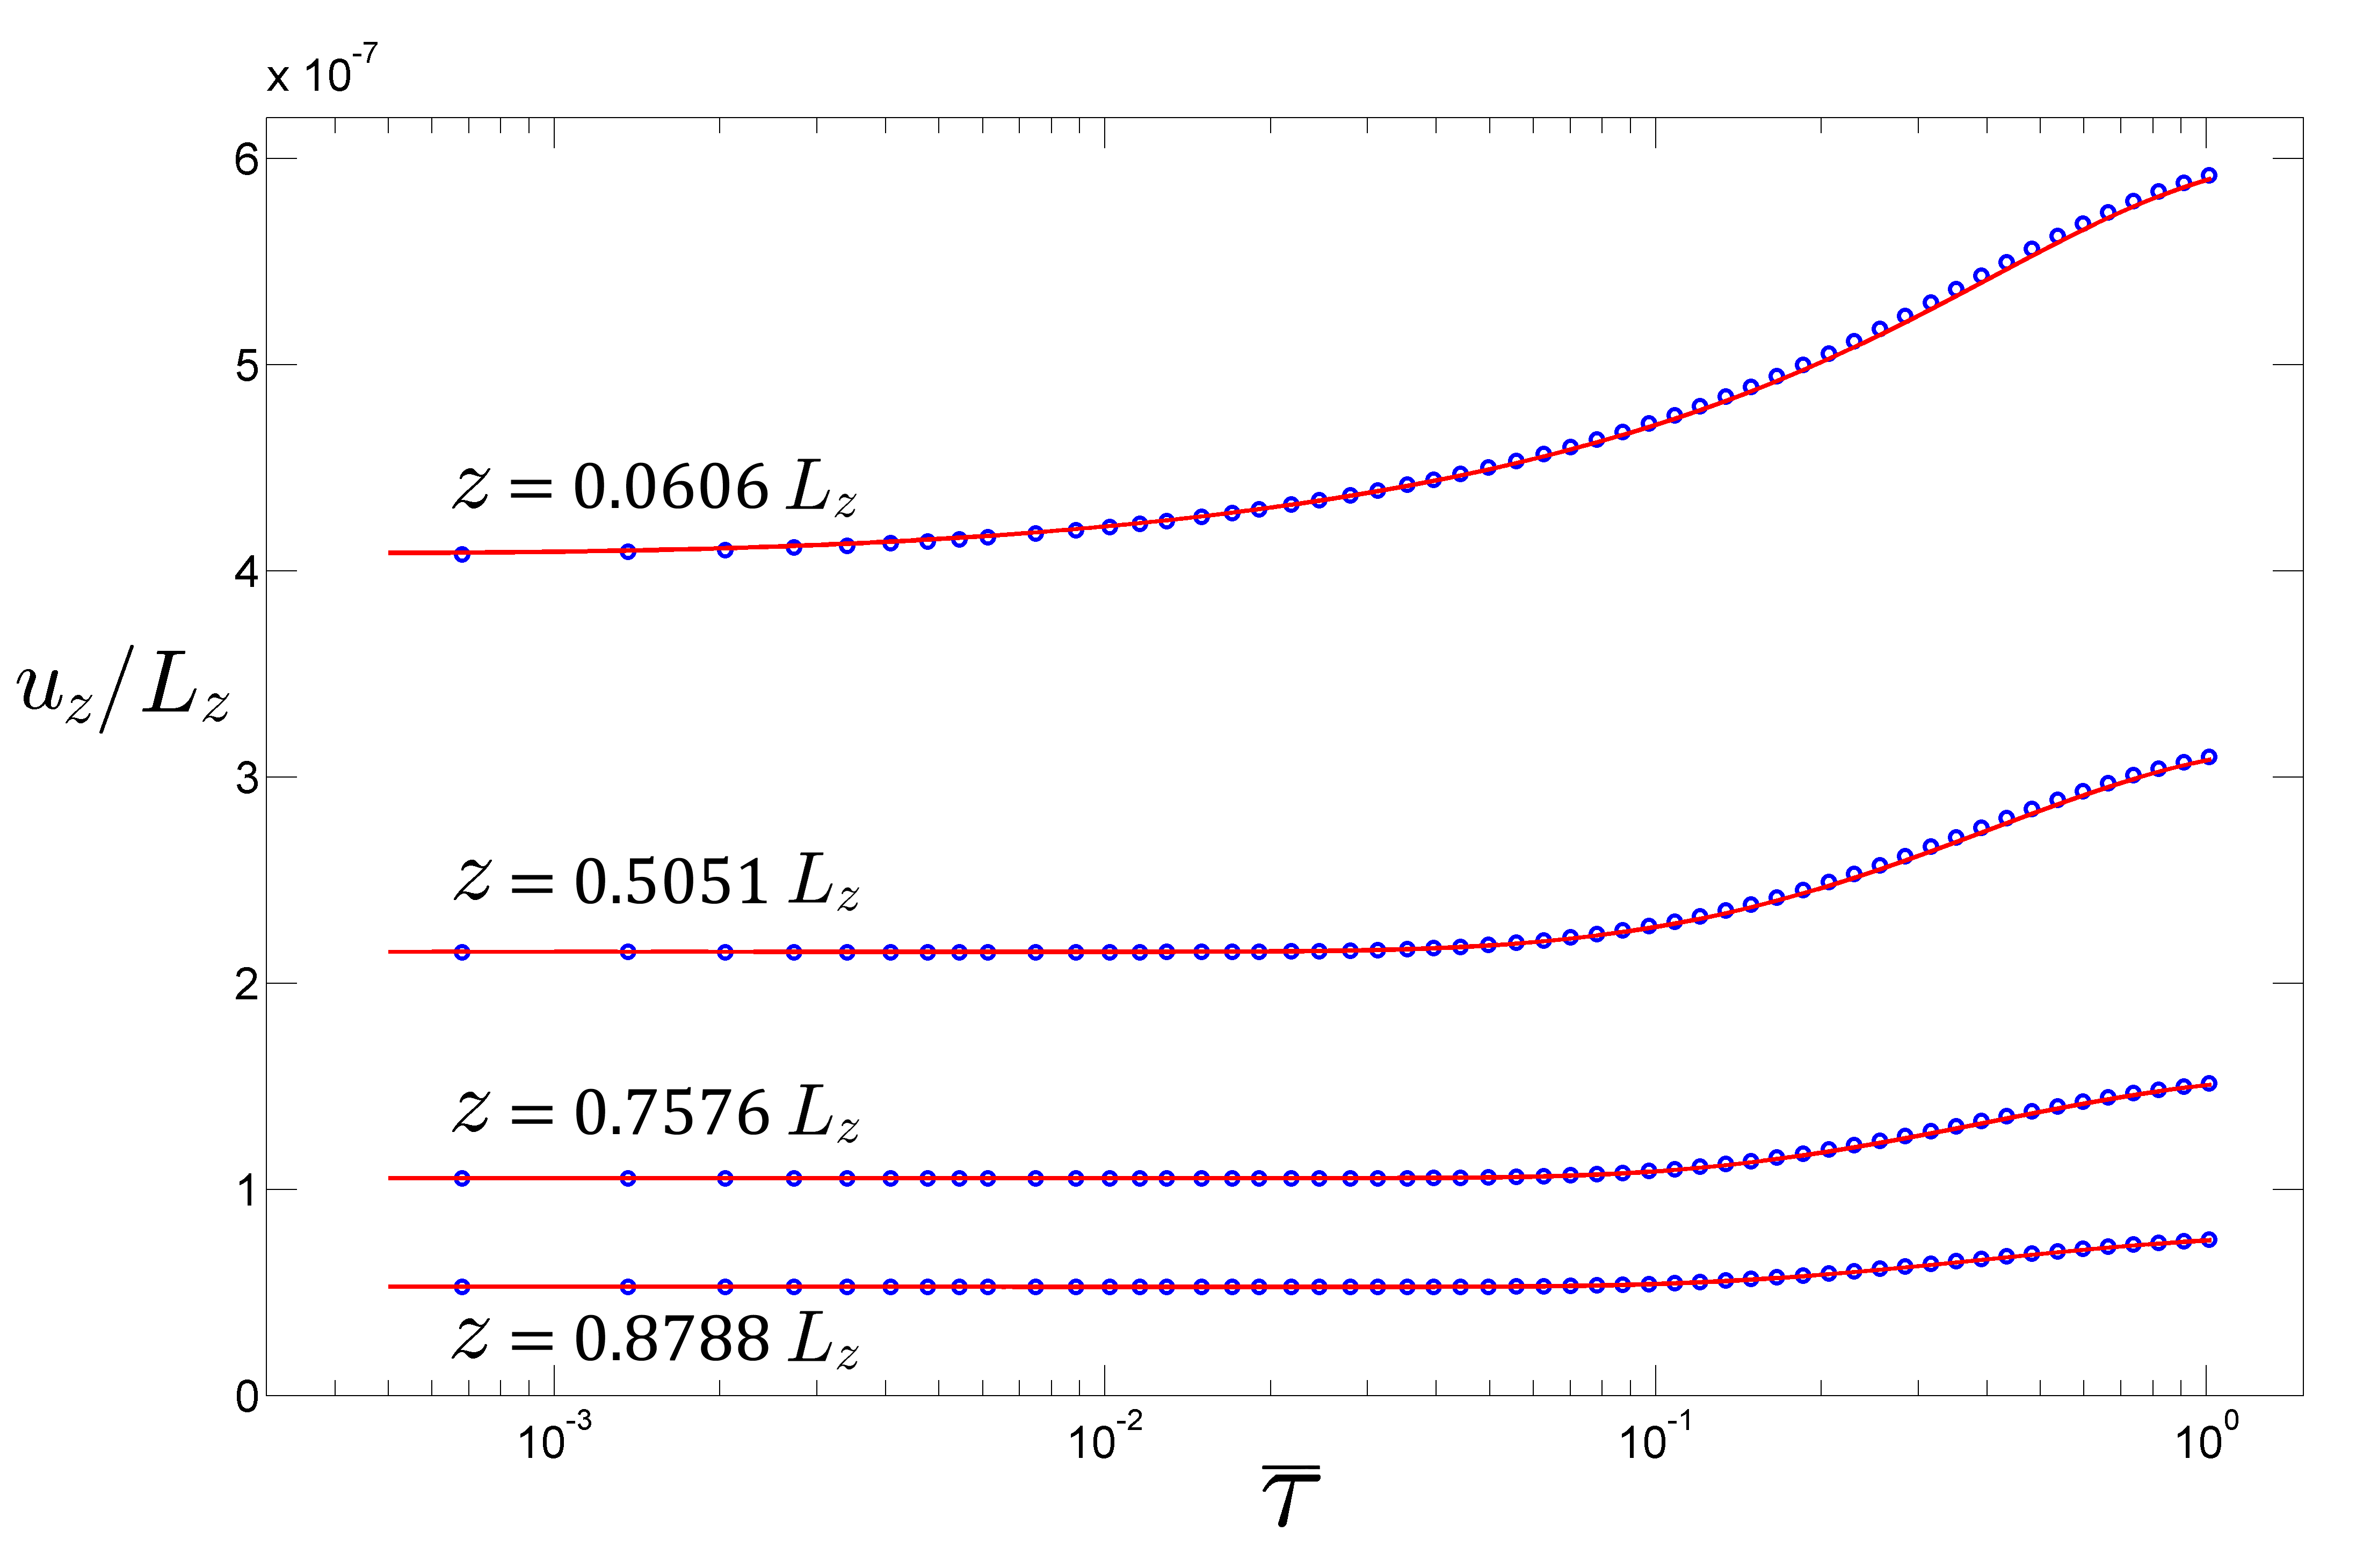
\includegraphics[width=0.9\textwidth]{./figs/uu0Ter.png}
% \caption{Нормированное перемещение в различные моменты времени: красным цветом показано
% аналитическое решение, синим~--- результаты расчета.}\label{fig:teru}
% \end{figure}
% 
 
На рис.~\ref{fig:terp} (вверху) показано распределение нормированного на начальную нагрузку $p_0$ давления $p$ в зависимости
от нормированной глубины $z/L_z$ в последовательные моменты времени $t = 5, \; 100, \; 500, \; 1000, \; 1500$ c.
Рис.~\ref{fig:terp} (внизу) демонстрирует нормированное на высоту колонны $L_z$
перемещение $u_z$ в зависимости от безразмерного времени $\overline{\tau}$ для нескольких выделенных глубин
$z/L_z = 0.0606, \; 0.5051, \; 0.7576, \; 0.8788$. На обоих рисунках красным цветом показано
соответствующие аналитическое решение, синим~-- результаты численного расчета, при этом данные для анализа брались в центральных точках области,
равноудаленных от боковых границ резервуара.
Как видно из представленных рисунков, расчеты продемонстрировали хорошее совпадение с аналитическими
данными. Также в качестве иллюстрации на рис.~\ref{fig:terpp}
%и~\ref{fig:teruu} 
приведены полученные в расчетах размерные распределения
полей давления $p$ и перемещения $u_z$ в последовательные моменты времени
$t = 100, \; 500, \; 1000, \; 1500$ c.

\begin{figure}[t!]
\centering
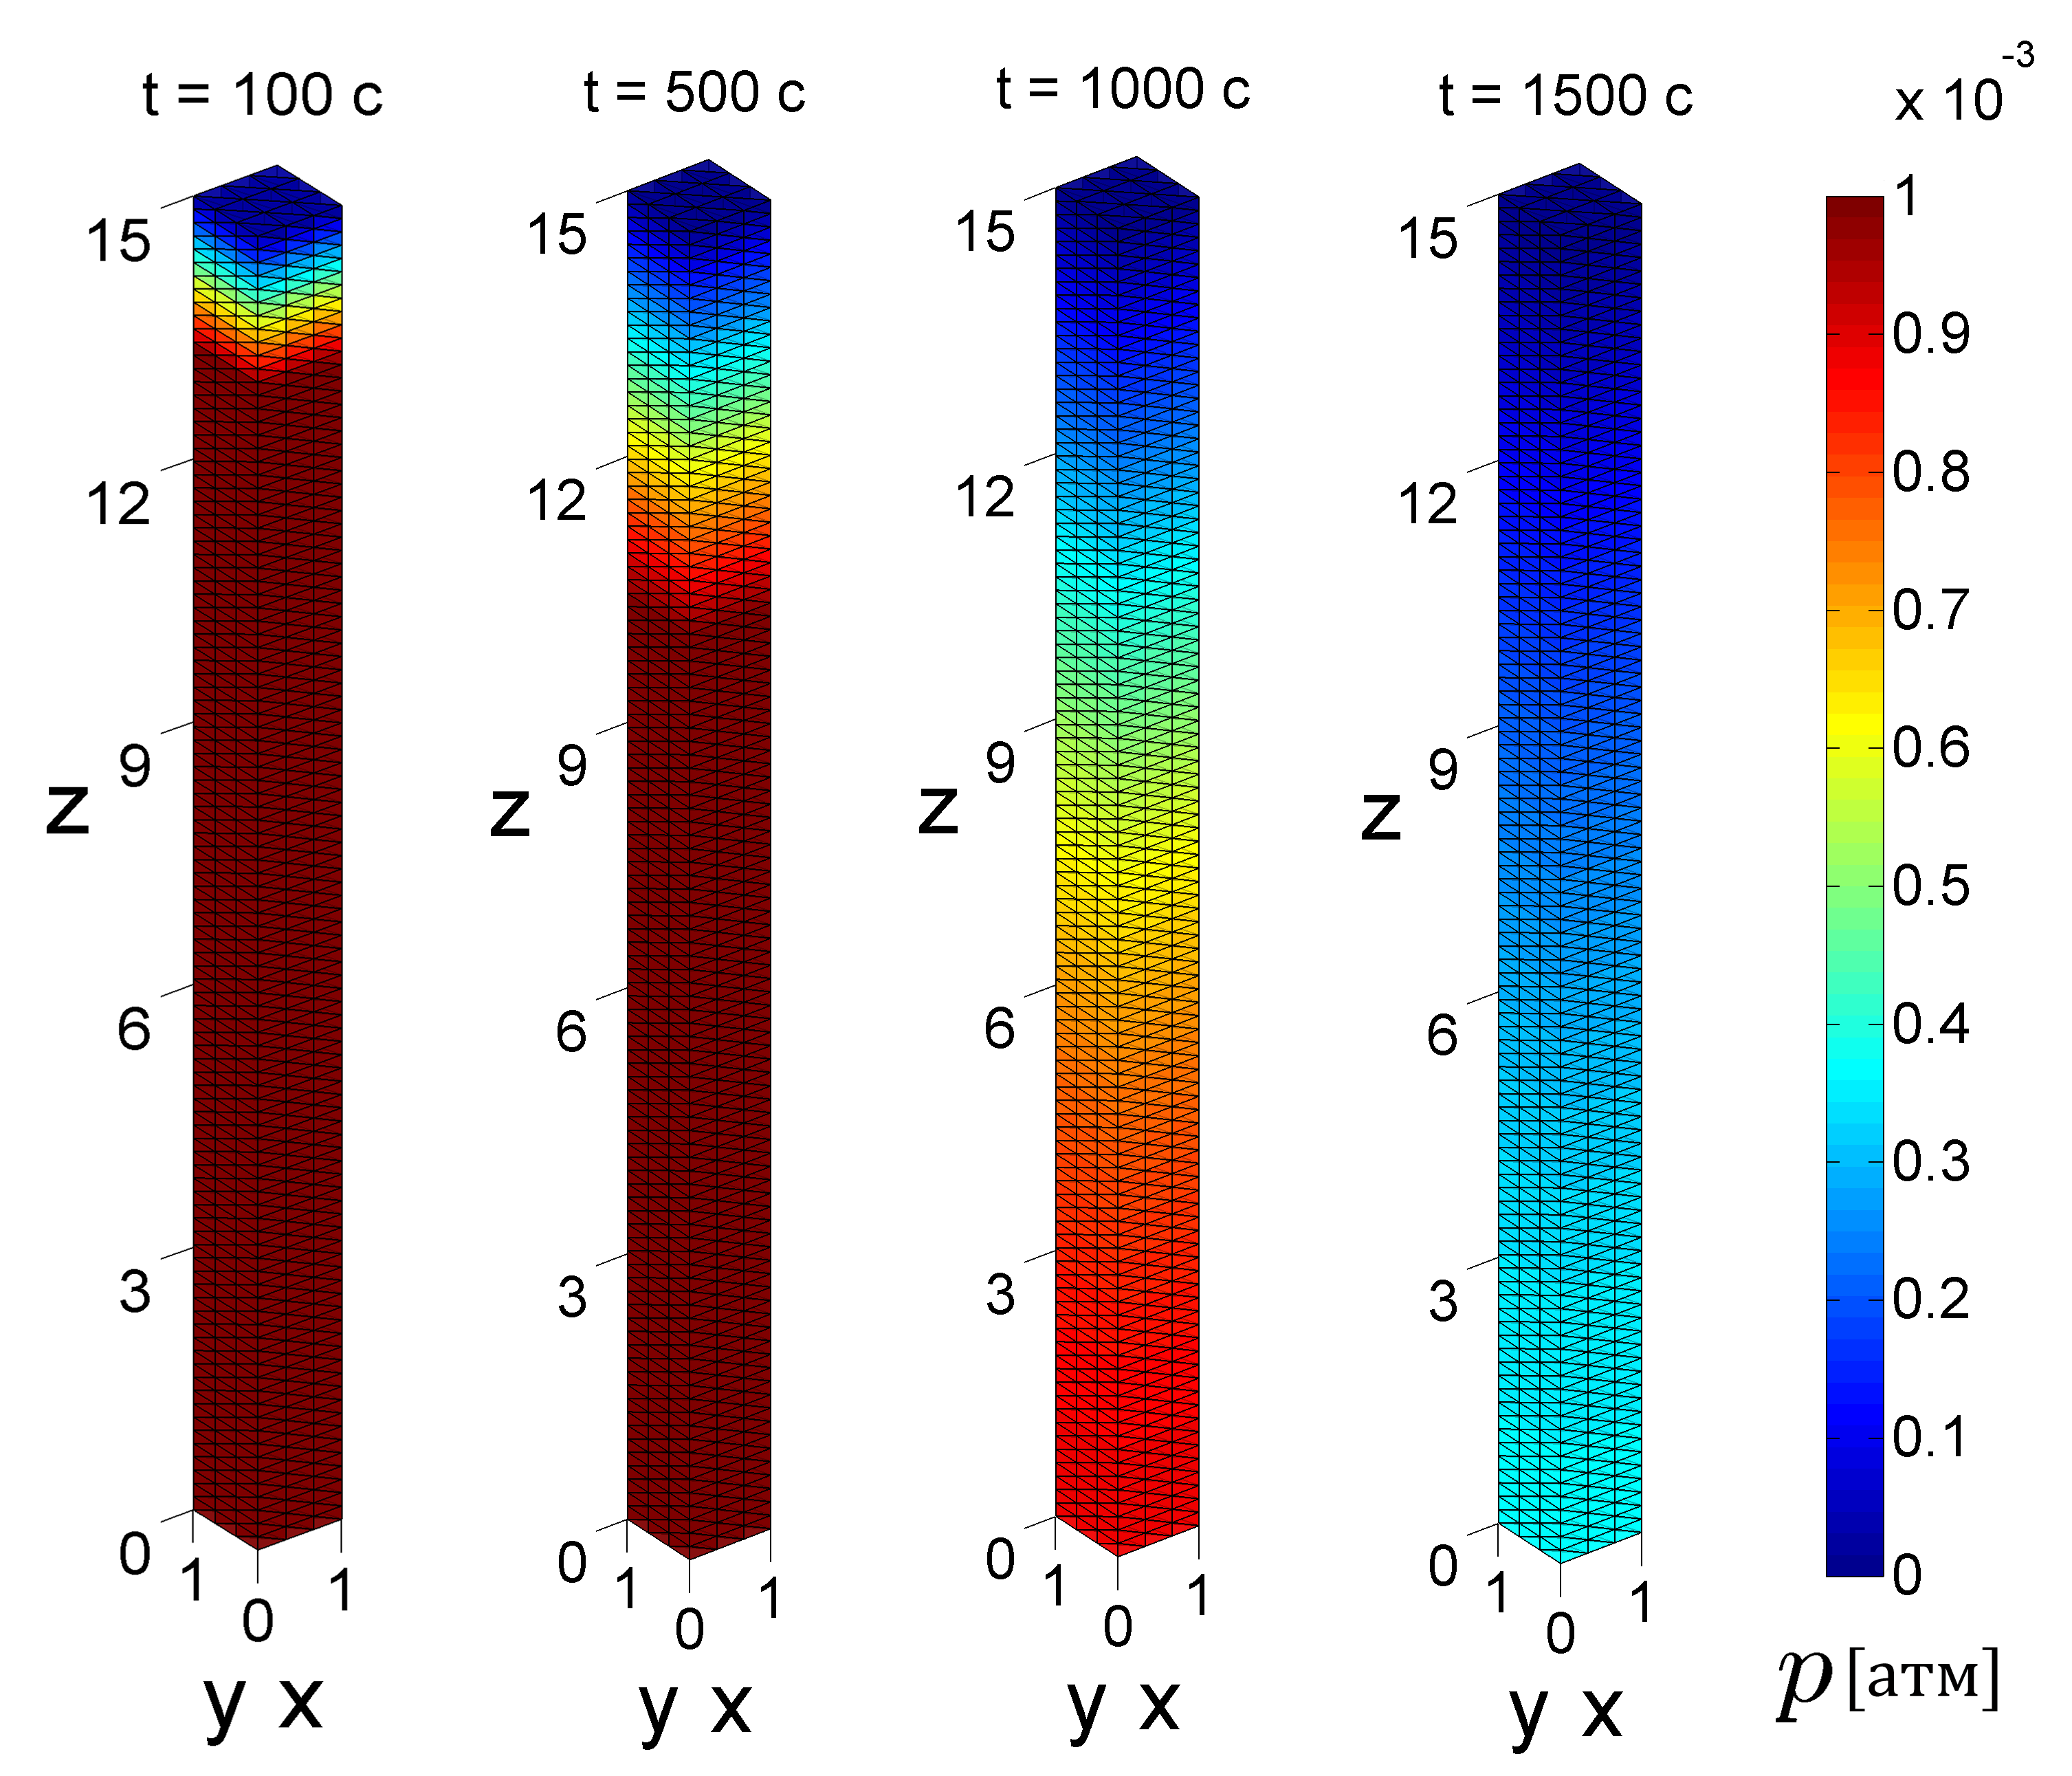
\includegraphics[width=0.75\textwidth]{./figs/pp1Ter.png}\\
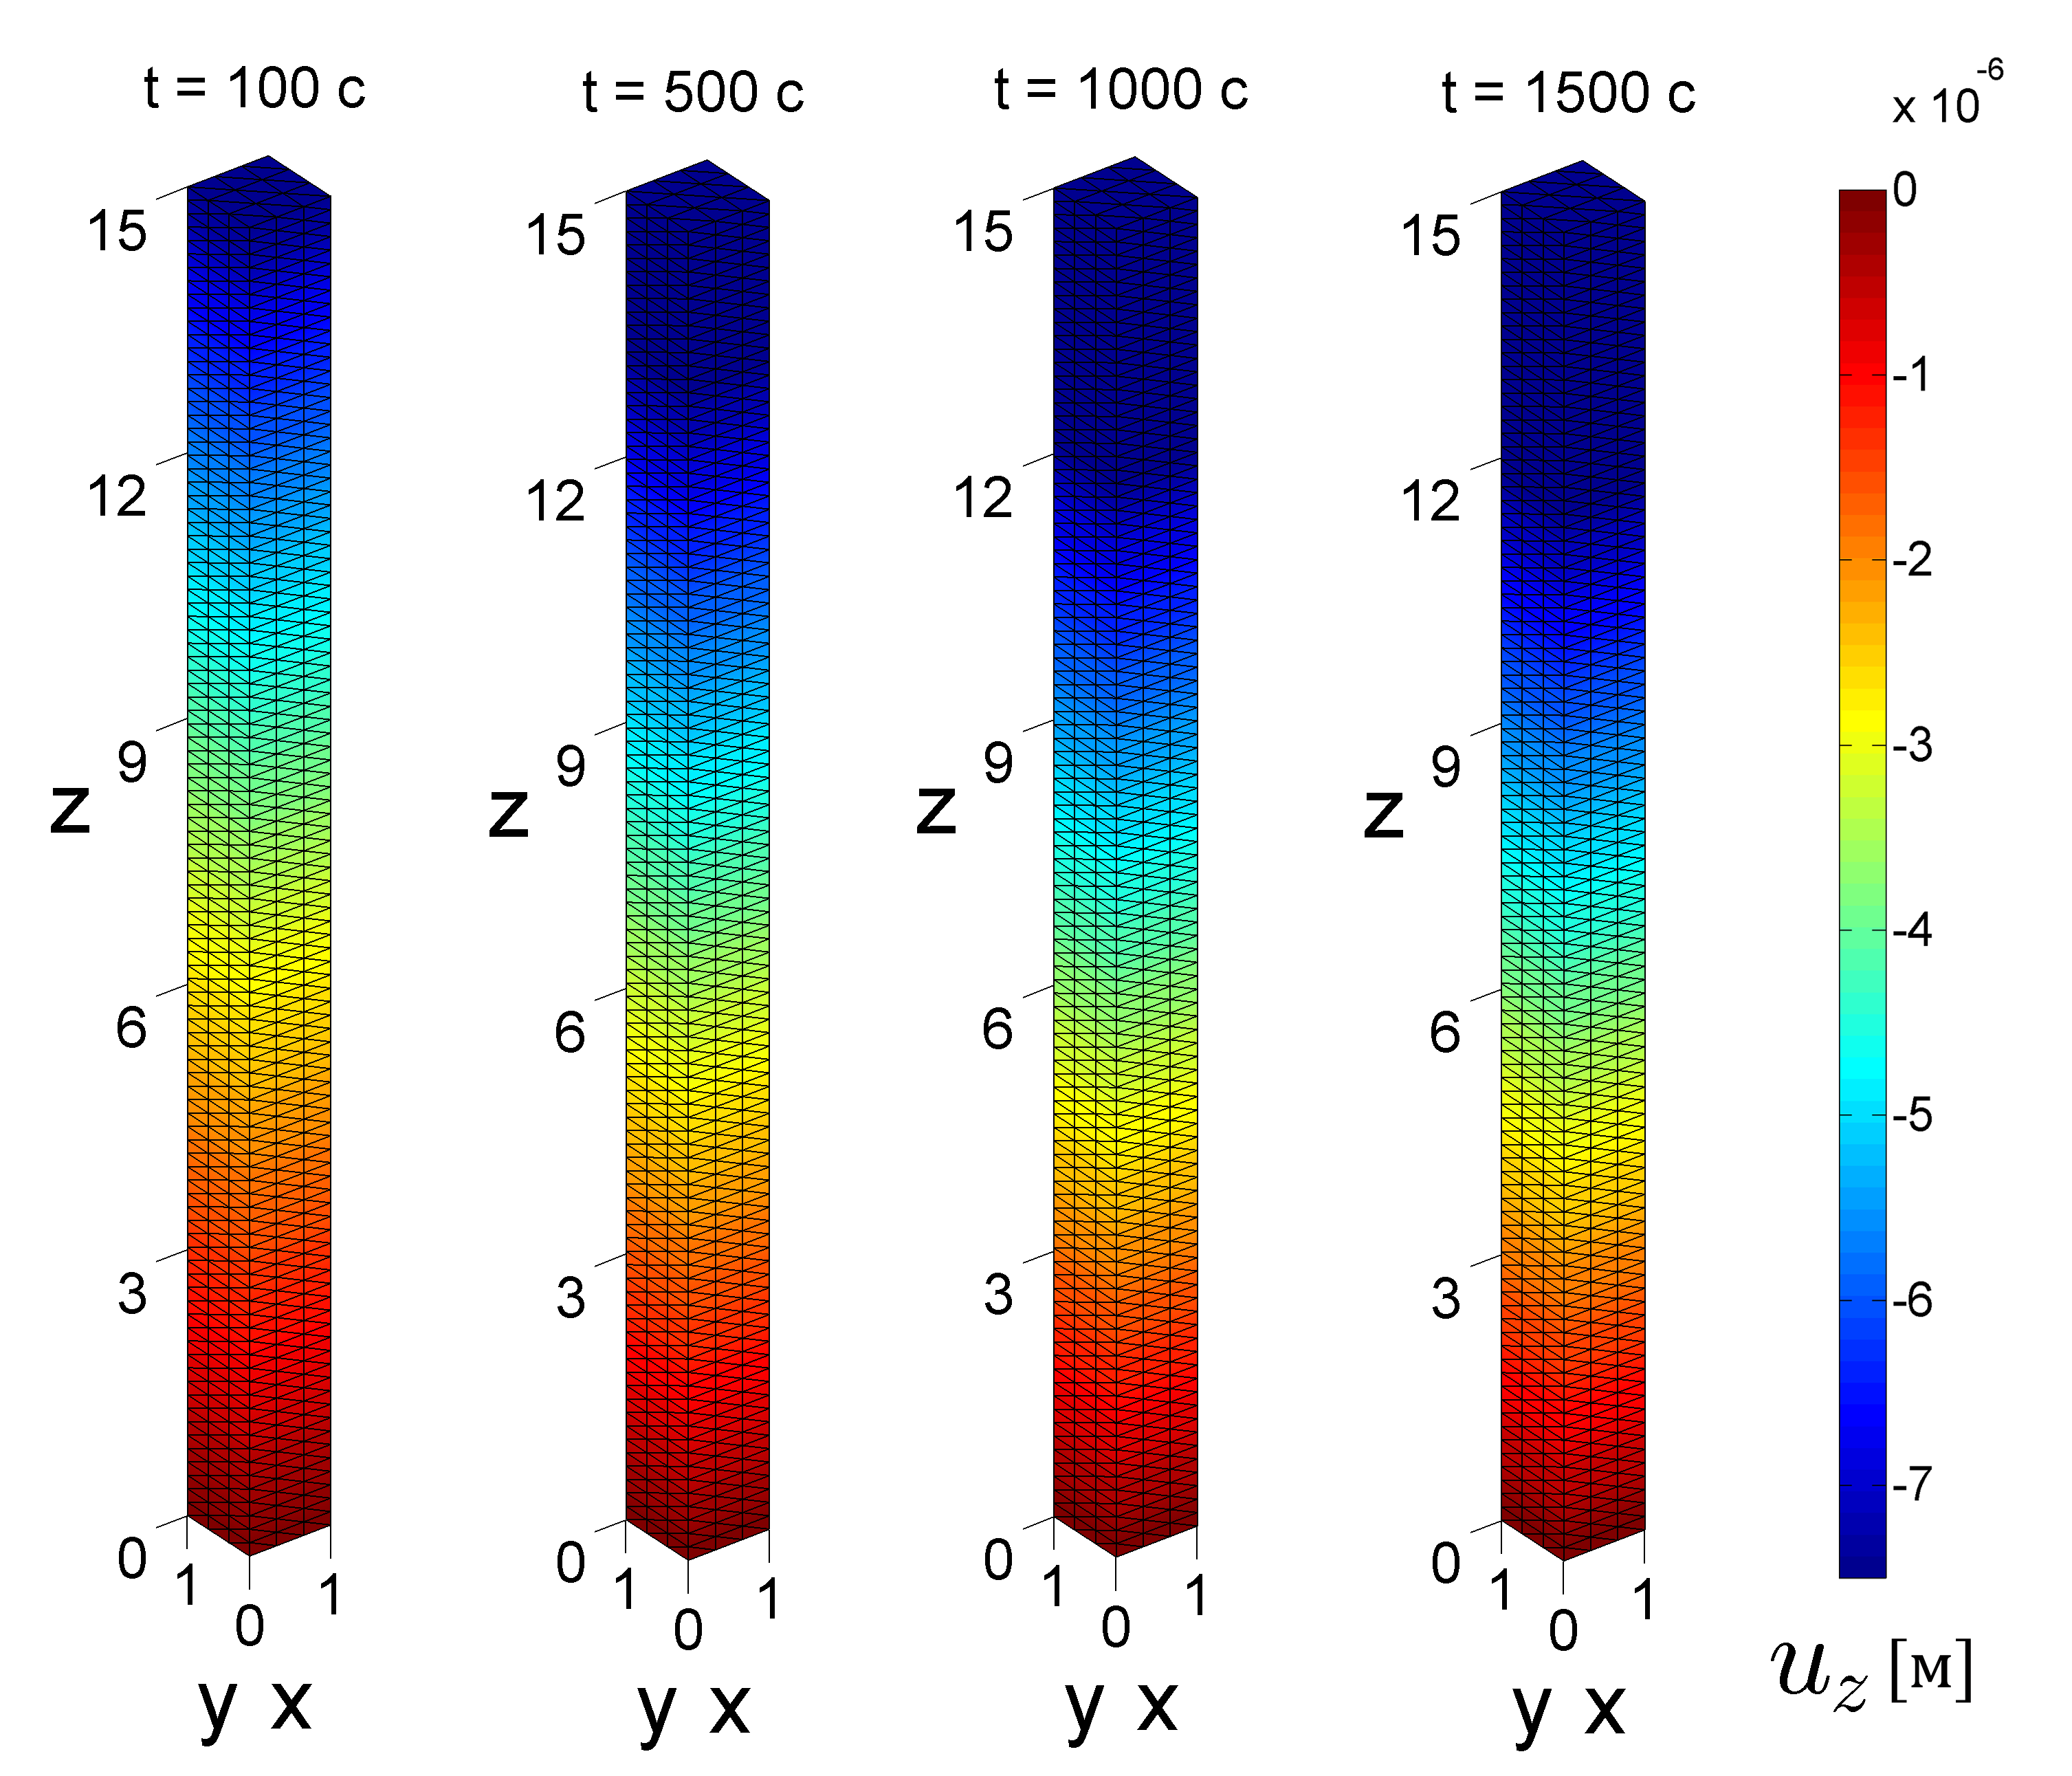
\includegraphics[width=0.75\textwidth]{./figs/uu1Ter.png}
\caption{ Задача консодидации Терцаги. Распределение давления (вверху) и перемещений $u_z$ (внизу) в 
последовательные моменты времени.}\label{fig:terpp}
\end{figure}
%
% \begin{figure}[b!]
% \centering
% 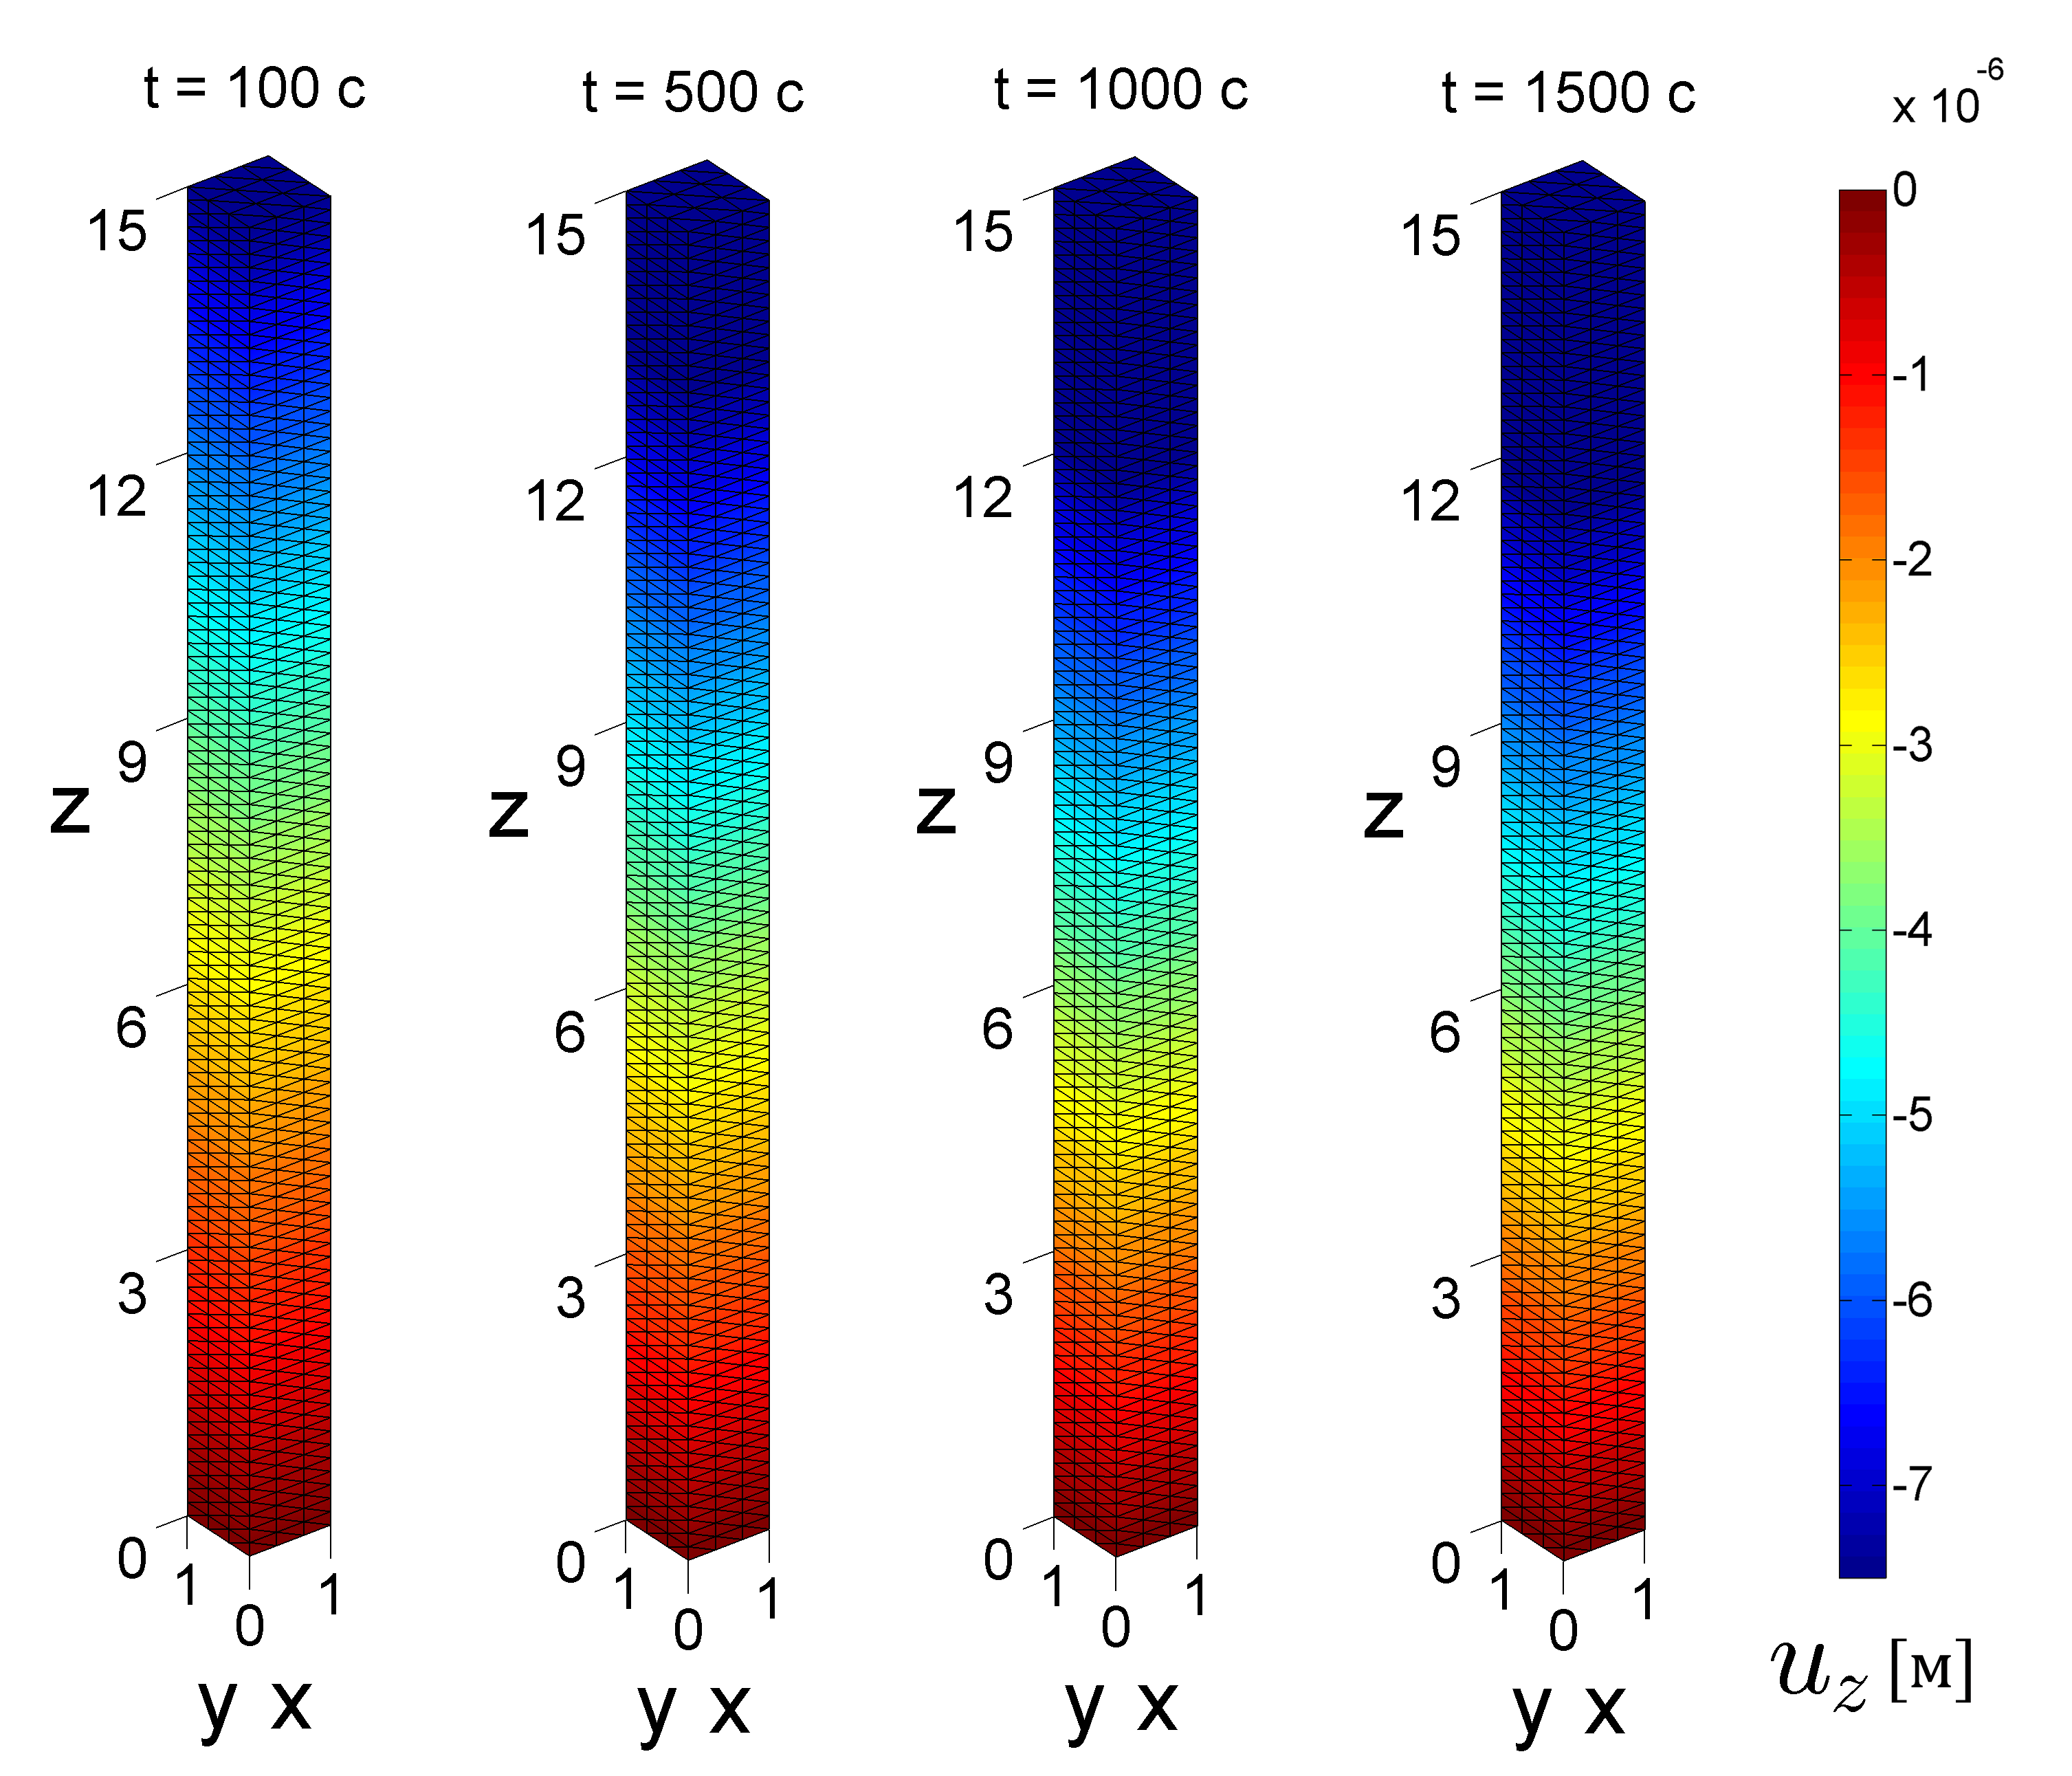
\includegraphics[width=0.95\textwidth]{./figs/uu1Ter.png}
% \caption{Распределение перемещений $u_z$ в последовательные моменты времени.}\label{fig:teruu}
% \end{figure}
% 

%\clearpage

\subsection{Задача Манделя}

Мандель в своей работе~\cite{mandel_1953} продемонстрировал классический
пример немонотонного поведения распределения порового давления по времени при недренированном нагружении
в условиях плоских деформаций.
В оригинальной постановке задача ставилась следующим образом. Рассматривалась насыщенная пороупругая среда
с линейными размерами $2a \times 2b$, зажатая между двумя жесткими непроницаемыми пластинами.
В начальный момент времени на пластины мгновенно начинала действовать сжимающая сила $F = -2\sigma_0a$,
нормированная на единичную длину в $z$ направлении и далее не меняющаяся со временем. 
Боковые границы области полагались свободно деформируемыми и проницаемыми, в начальный момент времени
среда покоилась. 

В силу симметрии задачи в настоящей работе для численных расчетов используется одна восьмая часть резервуара,
с началом координатам в центре исходной области. Также в отличие от оригинальной постановки предполагается,
что нагружение осуществляется в плоскости $Oxz$. Схематично задача представлена на рис.~\ref{fig:mandel}.
Здесь $L_x = a$ м, $L_z = b$ м, $T_z = -\sigma_0$.
%
\begin{figure}[h!]
\centering
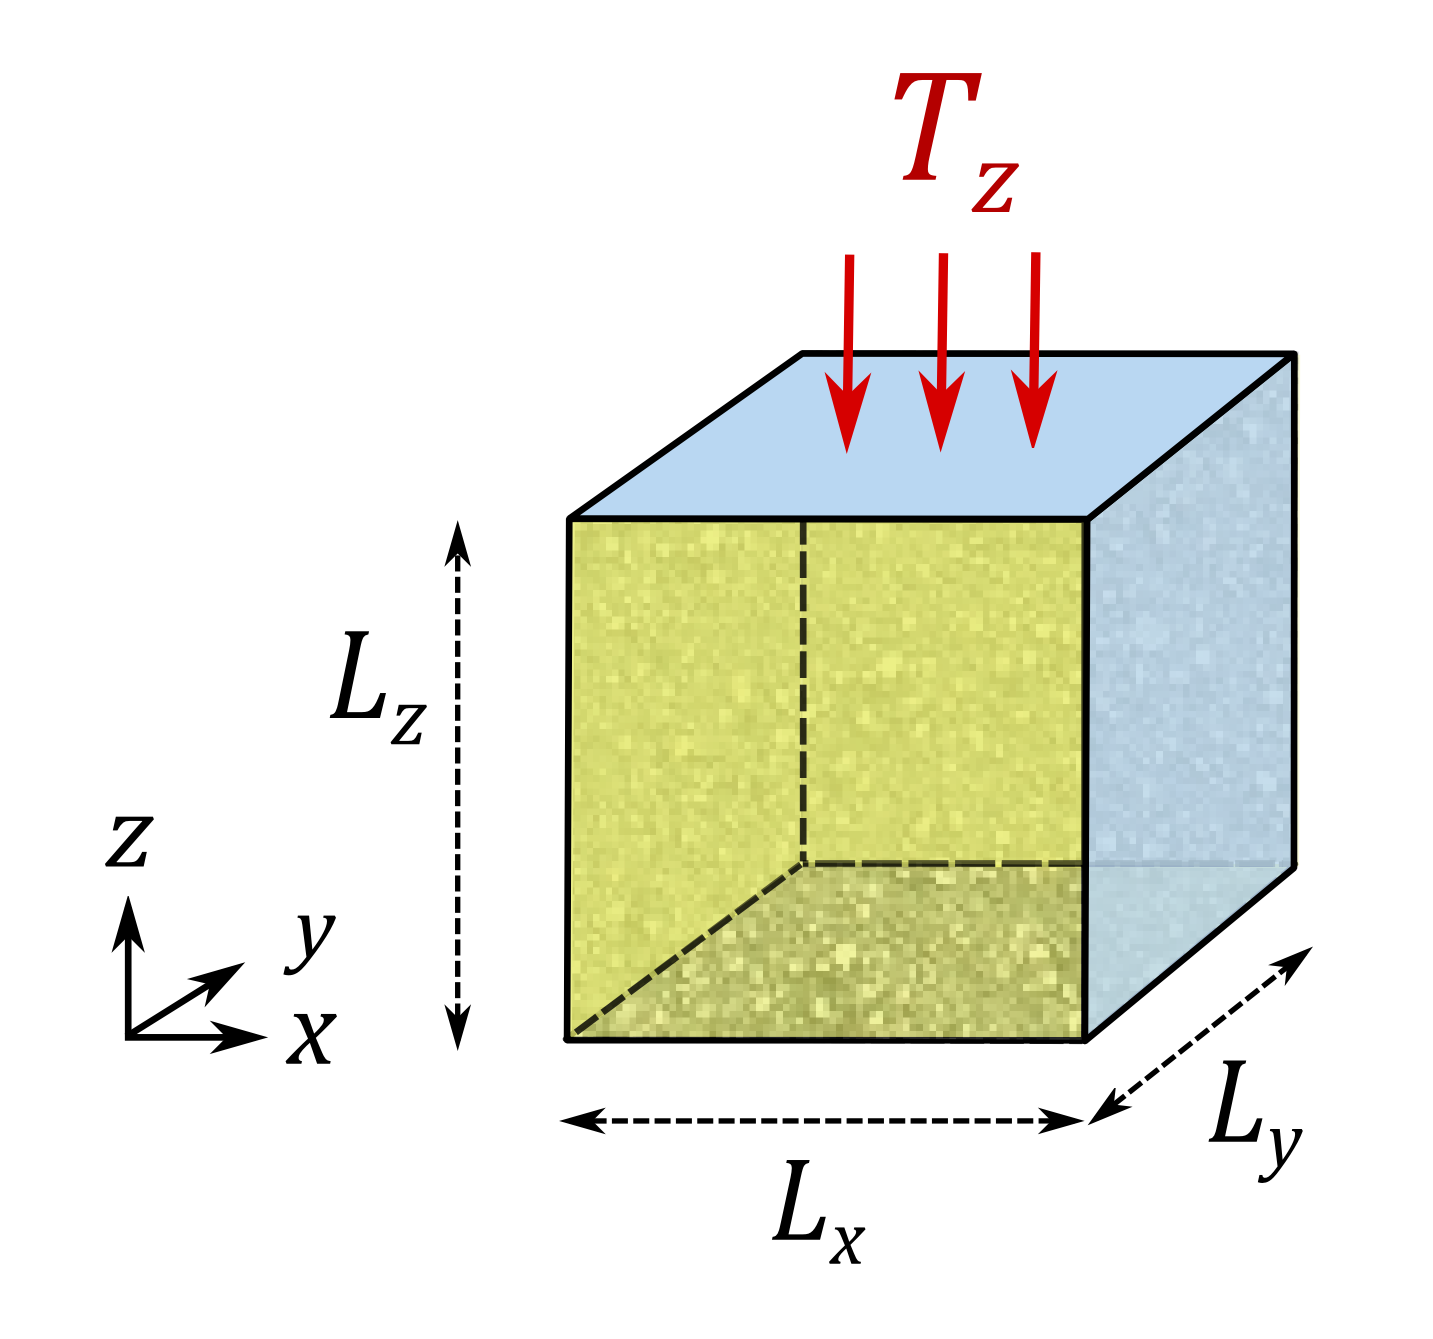
\includegraphics[width=0.65\textwidth]{./figs/mandel.png}
\caption{Схематичный вид задачи Манделя. Желтым цветом выделены плоскости
симметрии в соответствии с граничными условиями.}\label{fig:mandel}
\end{figure}
% 

Граничные условия в двумерной постановке ставятся следующим образом:
%
\begin{equation}
\begin{aligned}
\label{eq:bcMan}
%
& x = 0: & &u_x = 0, \;  \partial p / \partial x = 0, \\
& x = a: & &\sigma_{xx} = 0, \;p = 0,\\
%& y = 0:  u_y = 0, \; \partial p / \partial y = 0, \\
%& y = L_y: u_y = 0, \; \partial p / \partial y = 0, \\[7pt]
& z = 0: &  &u_z = 0, \; \partial p / \partial z = 0,\\
& z = b: &  &\int \limits_{0}^{a} \sigma_{zz}(x,b,t)\, dx = -\sigma_0 a, \; \partial p / \partial z = 0.
%
\end{aligned}
\end{equation}
%

Аналитическое решение представленной задачи в наиболее полном виде представлено в работе~\cite{cheng_1988}
и имеет вид:
%%
\begin{multline}
\label{eq:PMan}
%
p(x,t) = \frac23 \sigma_0 B (1+\nu_u) \sum \limits_{m=1}^{\infty} \cfrac{\sin \lambda_m}{\lambda_m - \sin\lambda_m \cos\lambda_m} \\
%
\cdot \left( \cos\cfrac{\lambda_m x}{a} -\cos \lambda_m \right)
\cdot \exp \left( -\cfrac{\lambda_m^2 ct}{a^2} \right),
%
\end{multline}
%%

%%
\begin{multline}
\label{eq:UrMan}
%
u_x(x,t) = 
\left[
\frac{\sigma_0 \nu}{2G} - \frac{\sigma_0 \nu_u}{G} \sum \limits_{m=1}^{\infty}
\cfrac{\sin \lambda_m \cos \lambda_m}{\lambda_m - \sin\lambda_m \cos\lambda_m}
\cdot \exp \left( -\cfrac{\lambda_m^2 ct}{a^2} \right) 
\right]\cdot x \\
%
+ \frac{\sigma_0 a}{G} 
\sum \limits_{m=1}^{\infty} \cfrac{\cos \lambda_m}{\lambda_m - \sin\lambda_m \cos\lambda_m}
\cdot \sin \frac{\lambda_m x}{a} \cdot \exp \left( -\cfrac{\lambda_m^2 ct}{a^2} \right),
%
\end{multline}
%%

%%
\begin{multline}
\label{eq:UzMan}
%
u_z(z,t) = 
\left[
- \frac{ \sigma_0 (1-\nu)}{2G} + \frac{\sigma_0 (1-\nu_u)}{G} \sum \limits_{m=1}^{\infty}
\cfrac{\sin \lambda_m \cos \lambda_m}{\lambda_m - \sin\lambda_m \cos\lambda_m} \right. \\
\left.
\cdot \exp \left( -\cfrac{\lambda_m^2 ct}{a^2} \right) 
\right]\cdot z,
%
\end{multline}
%%
где $\lambda_m$~-- решение соответствующего нелинейного уравнения
%%
\begin{equation}
\label{eq:ManNonLin}
%
\tg \lambda_m = \frac{1-\nu}{\nu_u - \nu} \,\lambda_m.
%
\end{equation}
%%

В качестве величин для сравнения используются 
нормированные значения $\overline{p}$, $\overline{u}_z$, $\overline{u}_x$:
%
\begin{equation*}
%
\overline{p} = \cfrac{p}{\sigma_0}, \quad \overline{u}_x = \cfrac{u_x}{a}, \quad \overline{u}_z = \cfrac{u_z}{b}, \quad
\overline{x} = \cfrac{x}{a}, \quad \overline{\tau} = \cfrac{ct}{a^2},
%
\end{equation*}
%
где 
$$
c = \cfrac{2kG(1-\nu)(\nu_u-\nu)}{\mu b^2 (1-2\nu)^2(1-\nu_u)}.
$$

Конкретные значения используемых для расчетов параметров приведены в табл.~\ref{tab:mandel}.
В качестве начальных данных брались значения, полученные из аналитического решения~\eqref{eq:PMan}--\eqref{eq:UzMan} на
момент времени $t_{\text{start}}$. Кроме того, вместо граничного условия~\eqref{eq:bcMan} для $\sigma_{zz}$ на плоскости $z = b$
использовались значения из аналитического решения~\eqref{eq:UzMan} для $u_z$.
%
%%
\begin{table}[h!]
\centering
%
\renewcommand{\arraystretch}{1.5}
\renewcommand{\tabcolsep}{6 pt} 
\begin{tabular}{|c|c|c|c|c|c|c|}
\hline
$L_x = a$ & $L_z = b$ & $L_y$ & $\sigma_0$ & $t_{\text{start}}$ & $t_{\text{end}}$ & $\Delta t$\\
\hline
 $1.0$ м & $1.0$ м & $1.0$ м & $1.0$ КПа & $3.125\times 10^{-3}$ с & $1.25$ с & $3.125\times 10^{-4}$ с\\
\hline
\end{tabular}
%
\caption{Параметры для численного расчета задачи Манделя.}\label{tab:mandel}
\end{table}
%%
%

Для численных расчетов использовалась тетраэдральная сетка, состоящая из 
$N_{nodes} = 2625$ узлов и $N_{elems} = 12096$ прямоугольных тетраэдров со сторонами
$h_x = 0.0417$, $h_y = 0.1667$, $h_z = 0.0714$ м. 

Для нахождения корней нелинейного уравнения~\eqref{eq:ManNonLin} использовался метод Ньютона.

На рис.~\ref{fig:manp} показано распределение нормированного на начальную нагрузку $\sigma_0$ давления $p$ в зависимости
от нормированной продольной координаты $x/a$ в последовательные моменты времени
$t = 6.25 \times 10^{-3}, 3.75 \times 10^{-2},\; 1.28\times 10^{-1}, \; 3.28\times 10^{-1},\; 6.25\times 10^{-1}$ c.
Отметим, что на малых временах давление растет выше значения, предсказанного эффектом Скемптона,
$p(0^+)/\sigma_0 = B(1+\nu_u)/3 = 0.2879$, что является отличительной особенностью данной задачи. 

Рис.~\ref{fig:manux} и~\ref{fig:manuz} демонстрируют нормированные
перемещения $u_x$ и $u_z$ соответственно. Распределение $u_x$ бралось в плоскости $y=0.5/b$,
$u_z$~-- в плоскости $x=0.5/a$.
На всех рисунках красным цветом показаны
соответствующие аналитические решения, синим~-- результаты численного расчета.

Как видно из представленных результатов, расчеты продемонстрировали отличное совпадение с аналитическими
данными для всех моментов времени, в точности воспроизведя характерные особенности задачи. 

Также в качестве иллюстрации на рис.~\ref{fig:manpp} приведено полученное в расчетах размерное распределение
поля давления $p$ в последовательные моменты времени
$t = 3.75 \times 10^{-2},\; 1.28\times 10^{-1}, \; 3.28\times 10^{-1},\; 6.25\times 10^{-1}$ c.

%
\begin{figure}[t!]
\centering
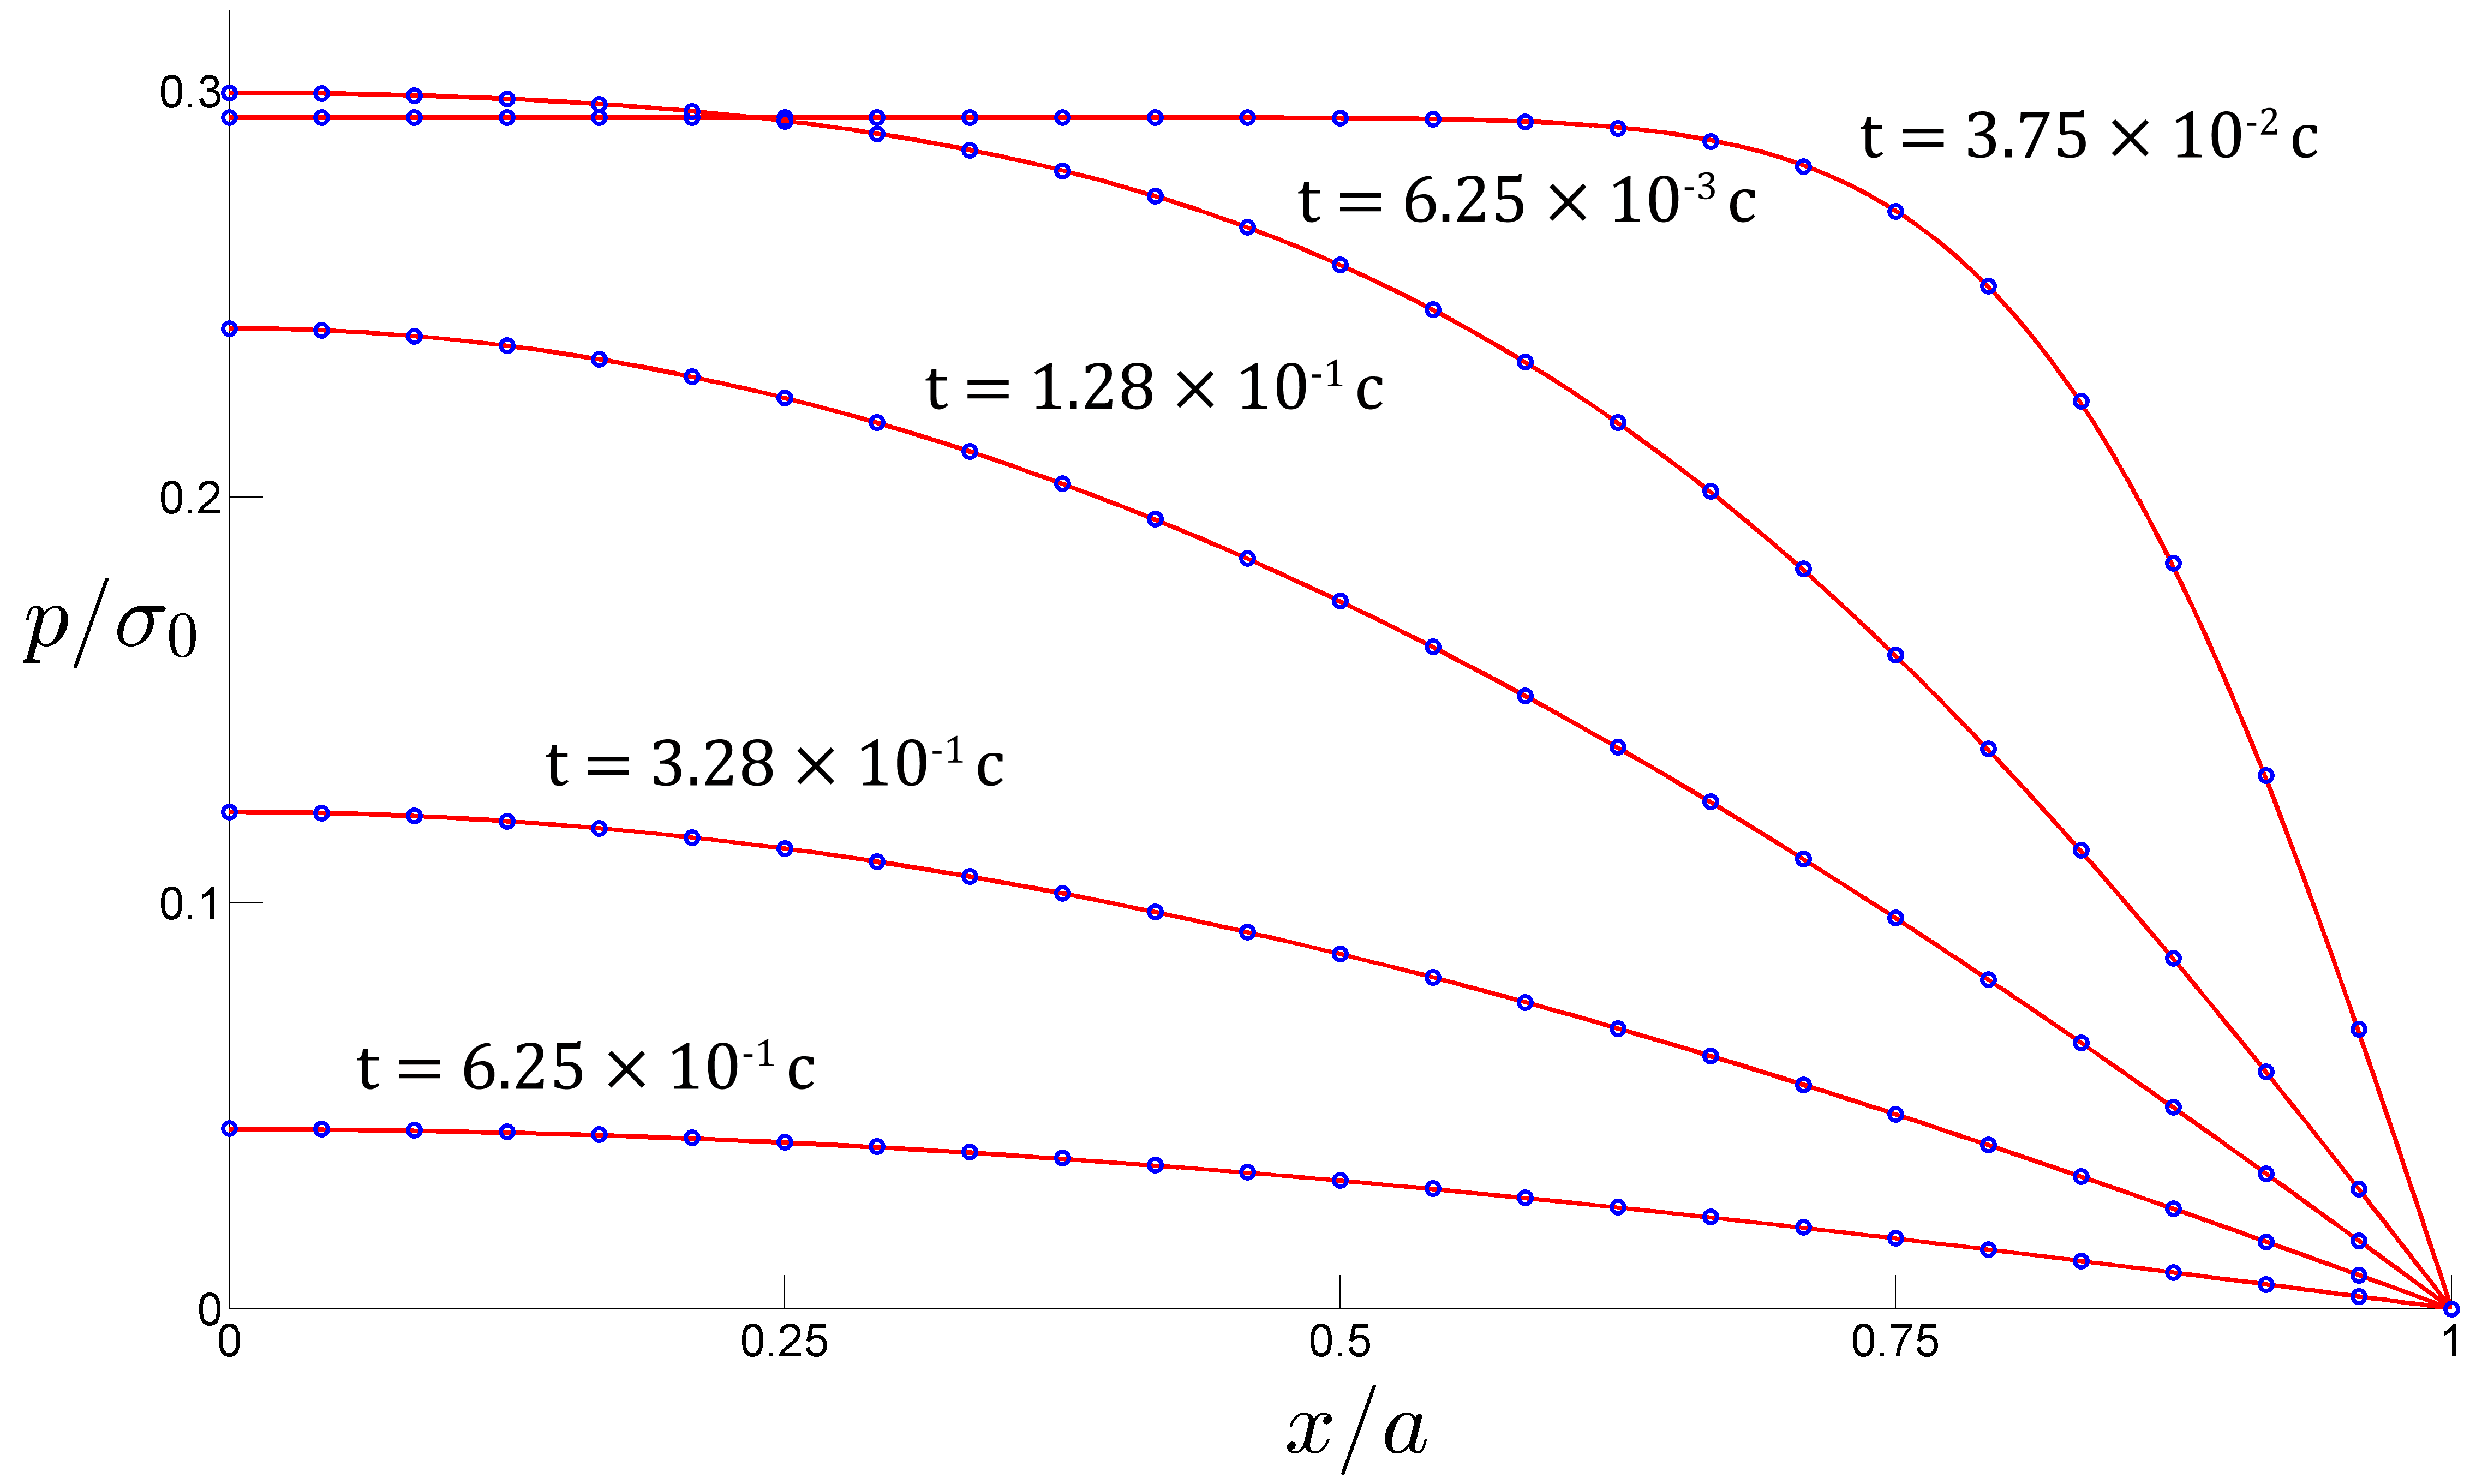
\includegraphics[width=0.95\textwidth]{./figs/pp0M.png}
\caption{Задача Манделя. Нормированное давление в различные моменты времени: красным цветом показано
аналитическое решение, синим~--- результаты расчета.}\label{fig:manp}
\end{figure}
% 
%
\begin{figure}[h!]
\centering
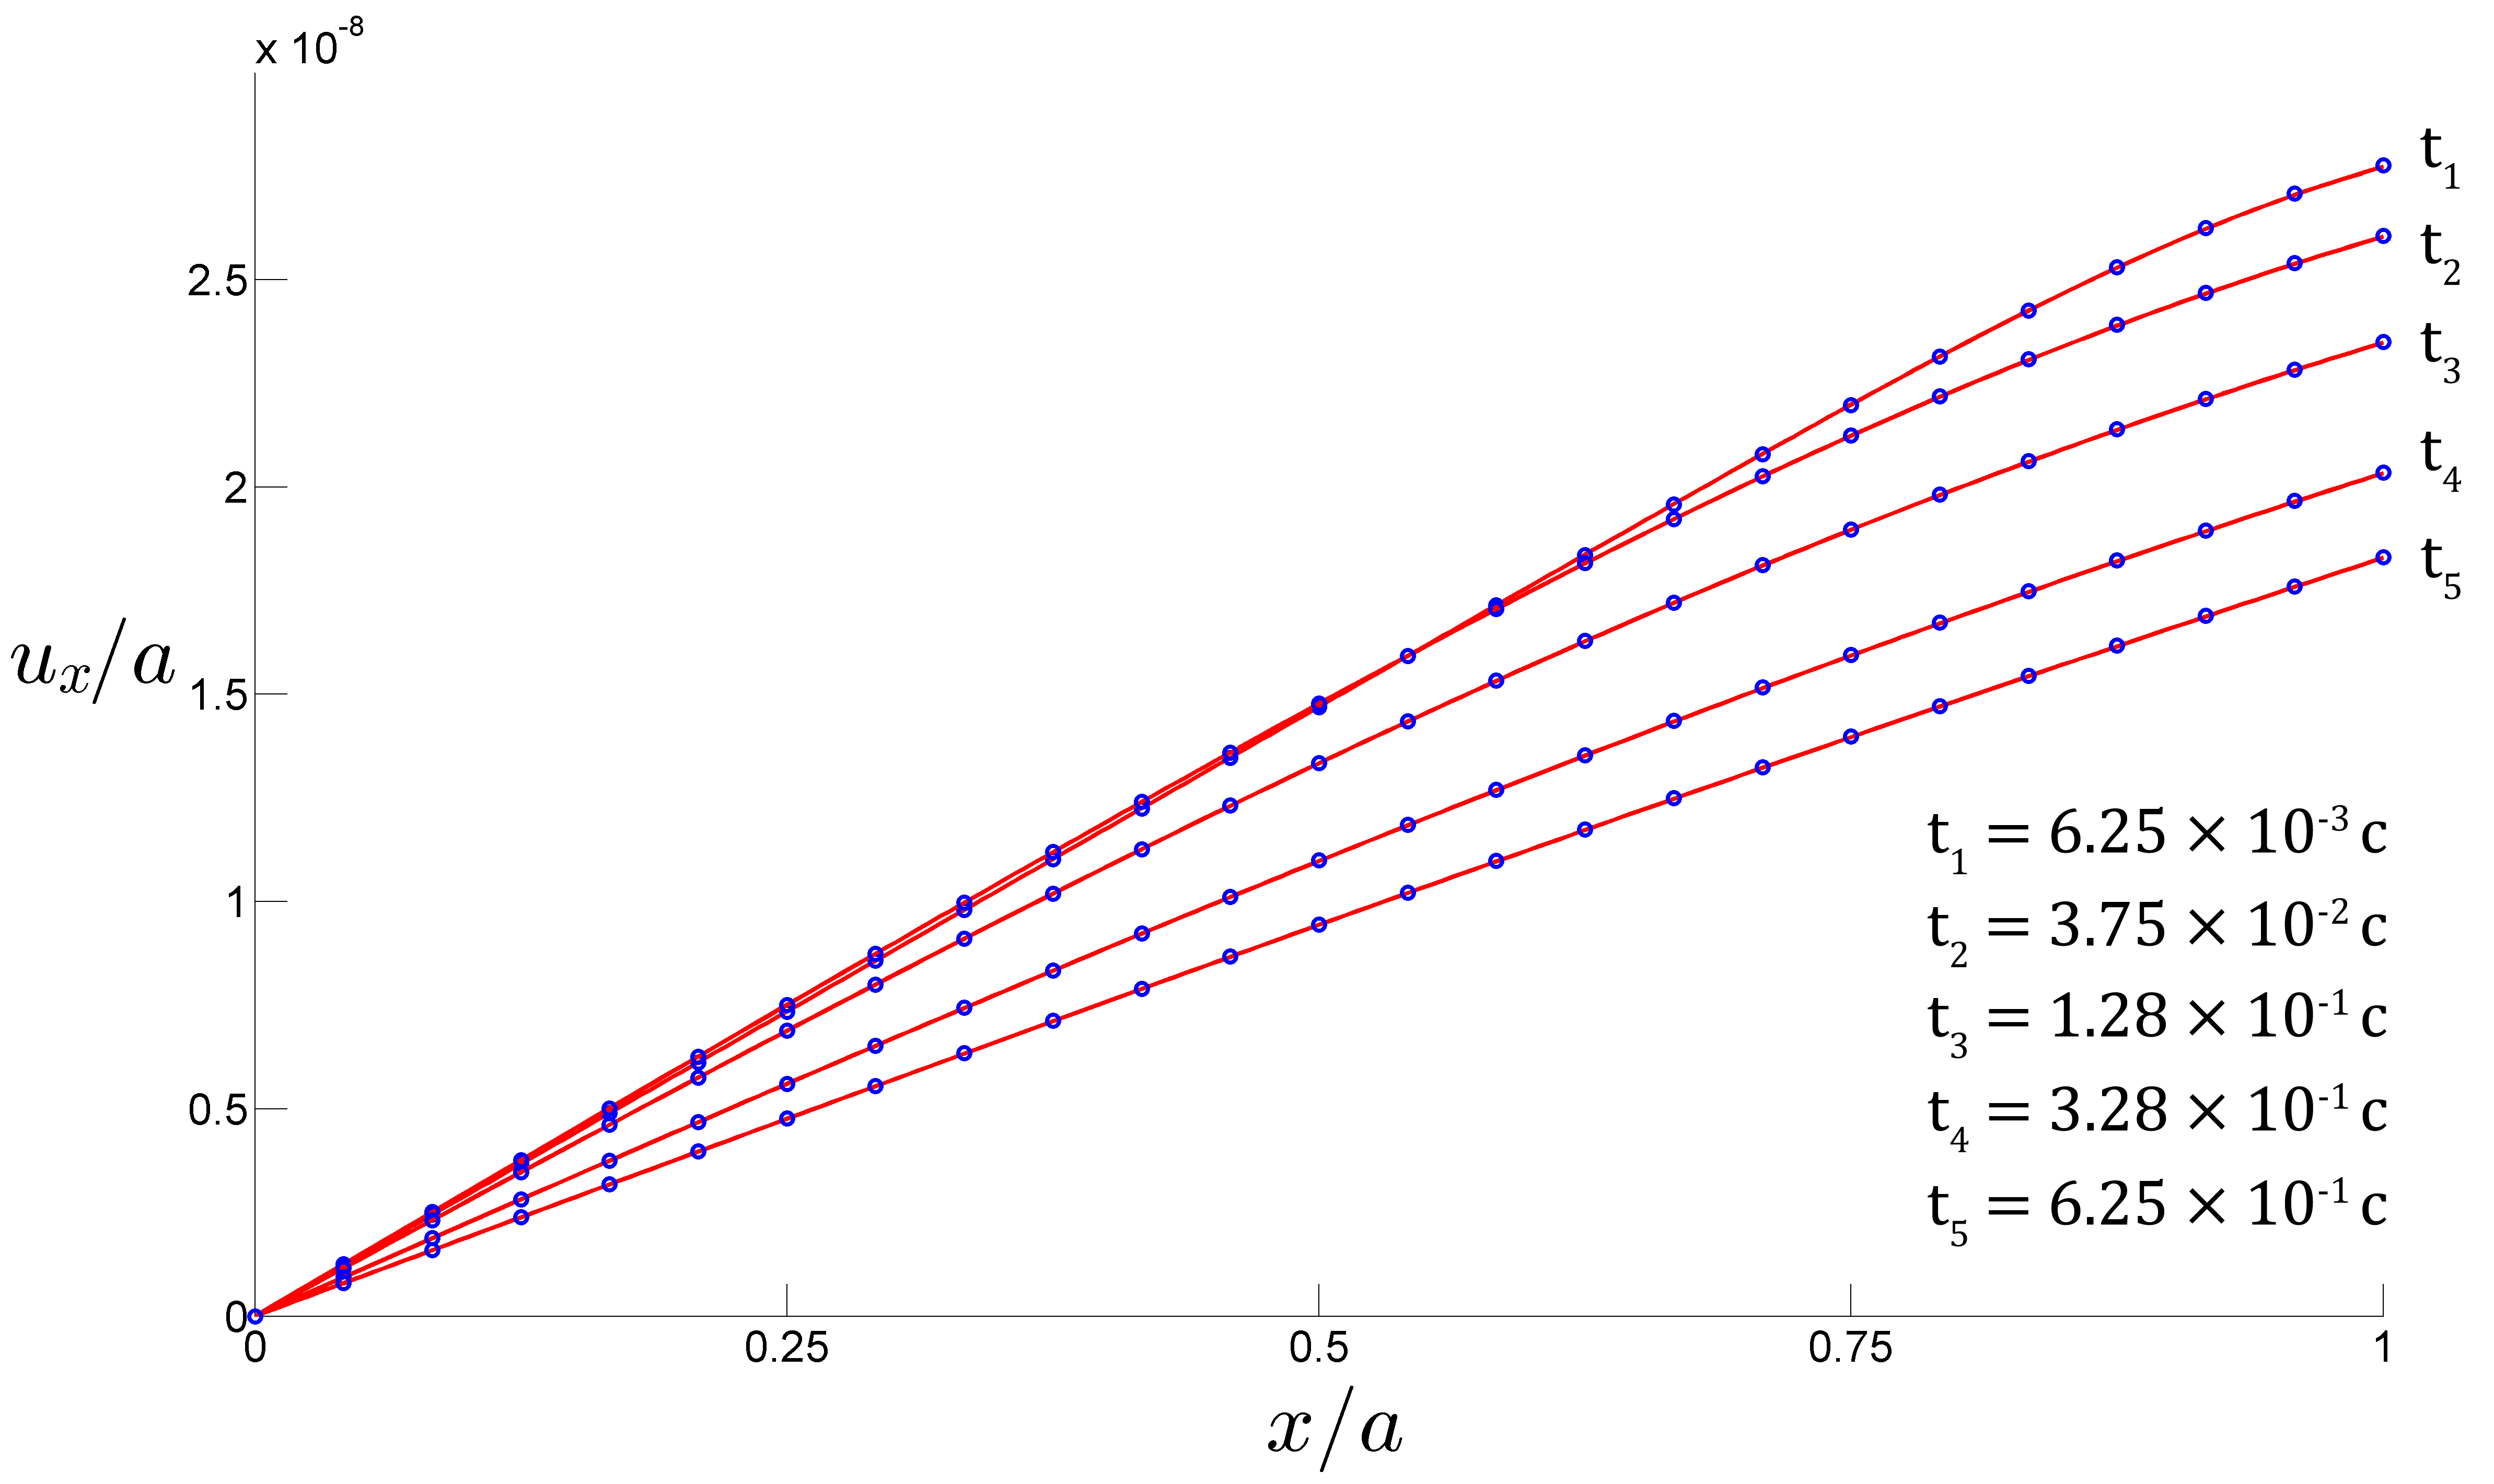
\includegraphics[width=0.85\textwidth]{./figs/uux0M.png}
\caption{ Задача Манделя. Нормированное перемещение $u_x$ в различные моменты времени: красным цветом показано
аналитическое решение, синим~--- результаты расчета.}\label{fig:manux}
\end{figure}
%
%
\begin{figure}[t!]
\centering
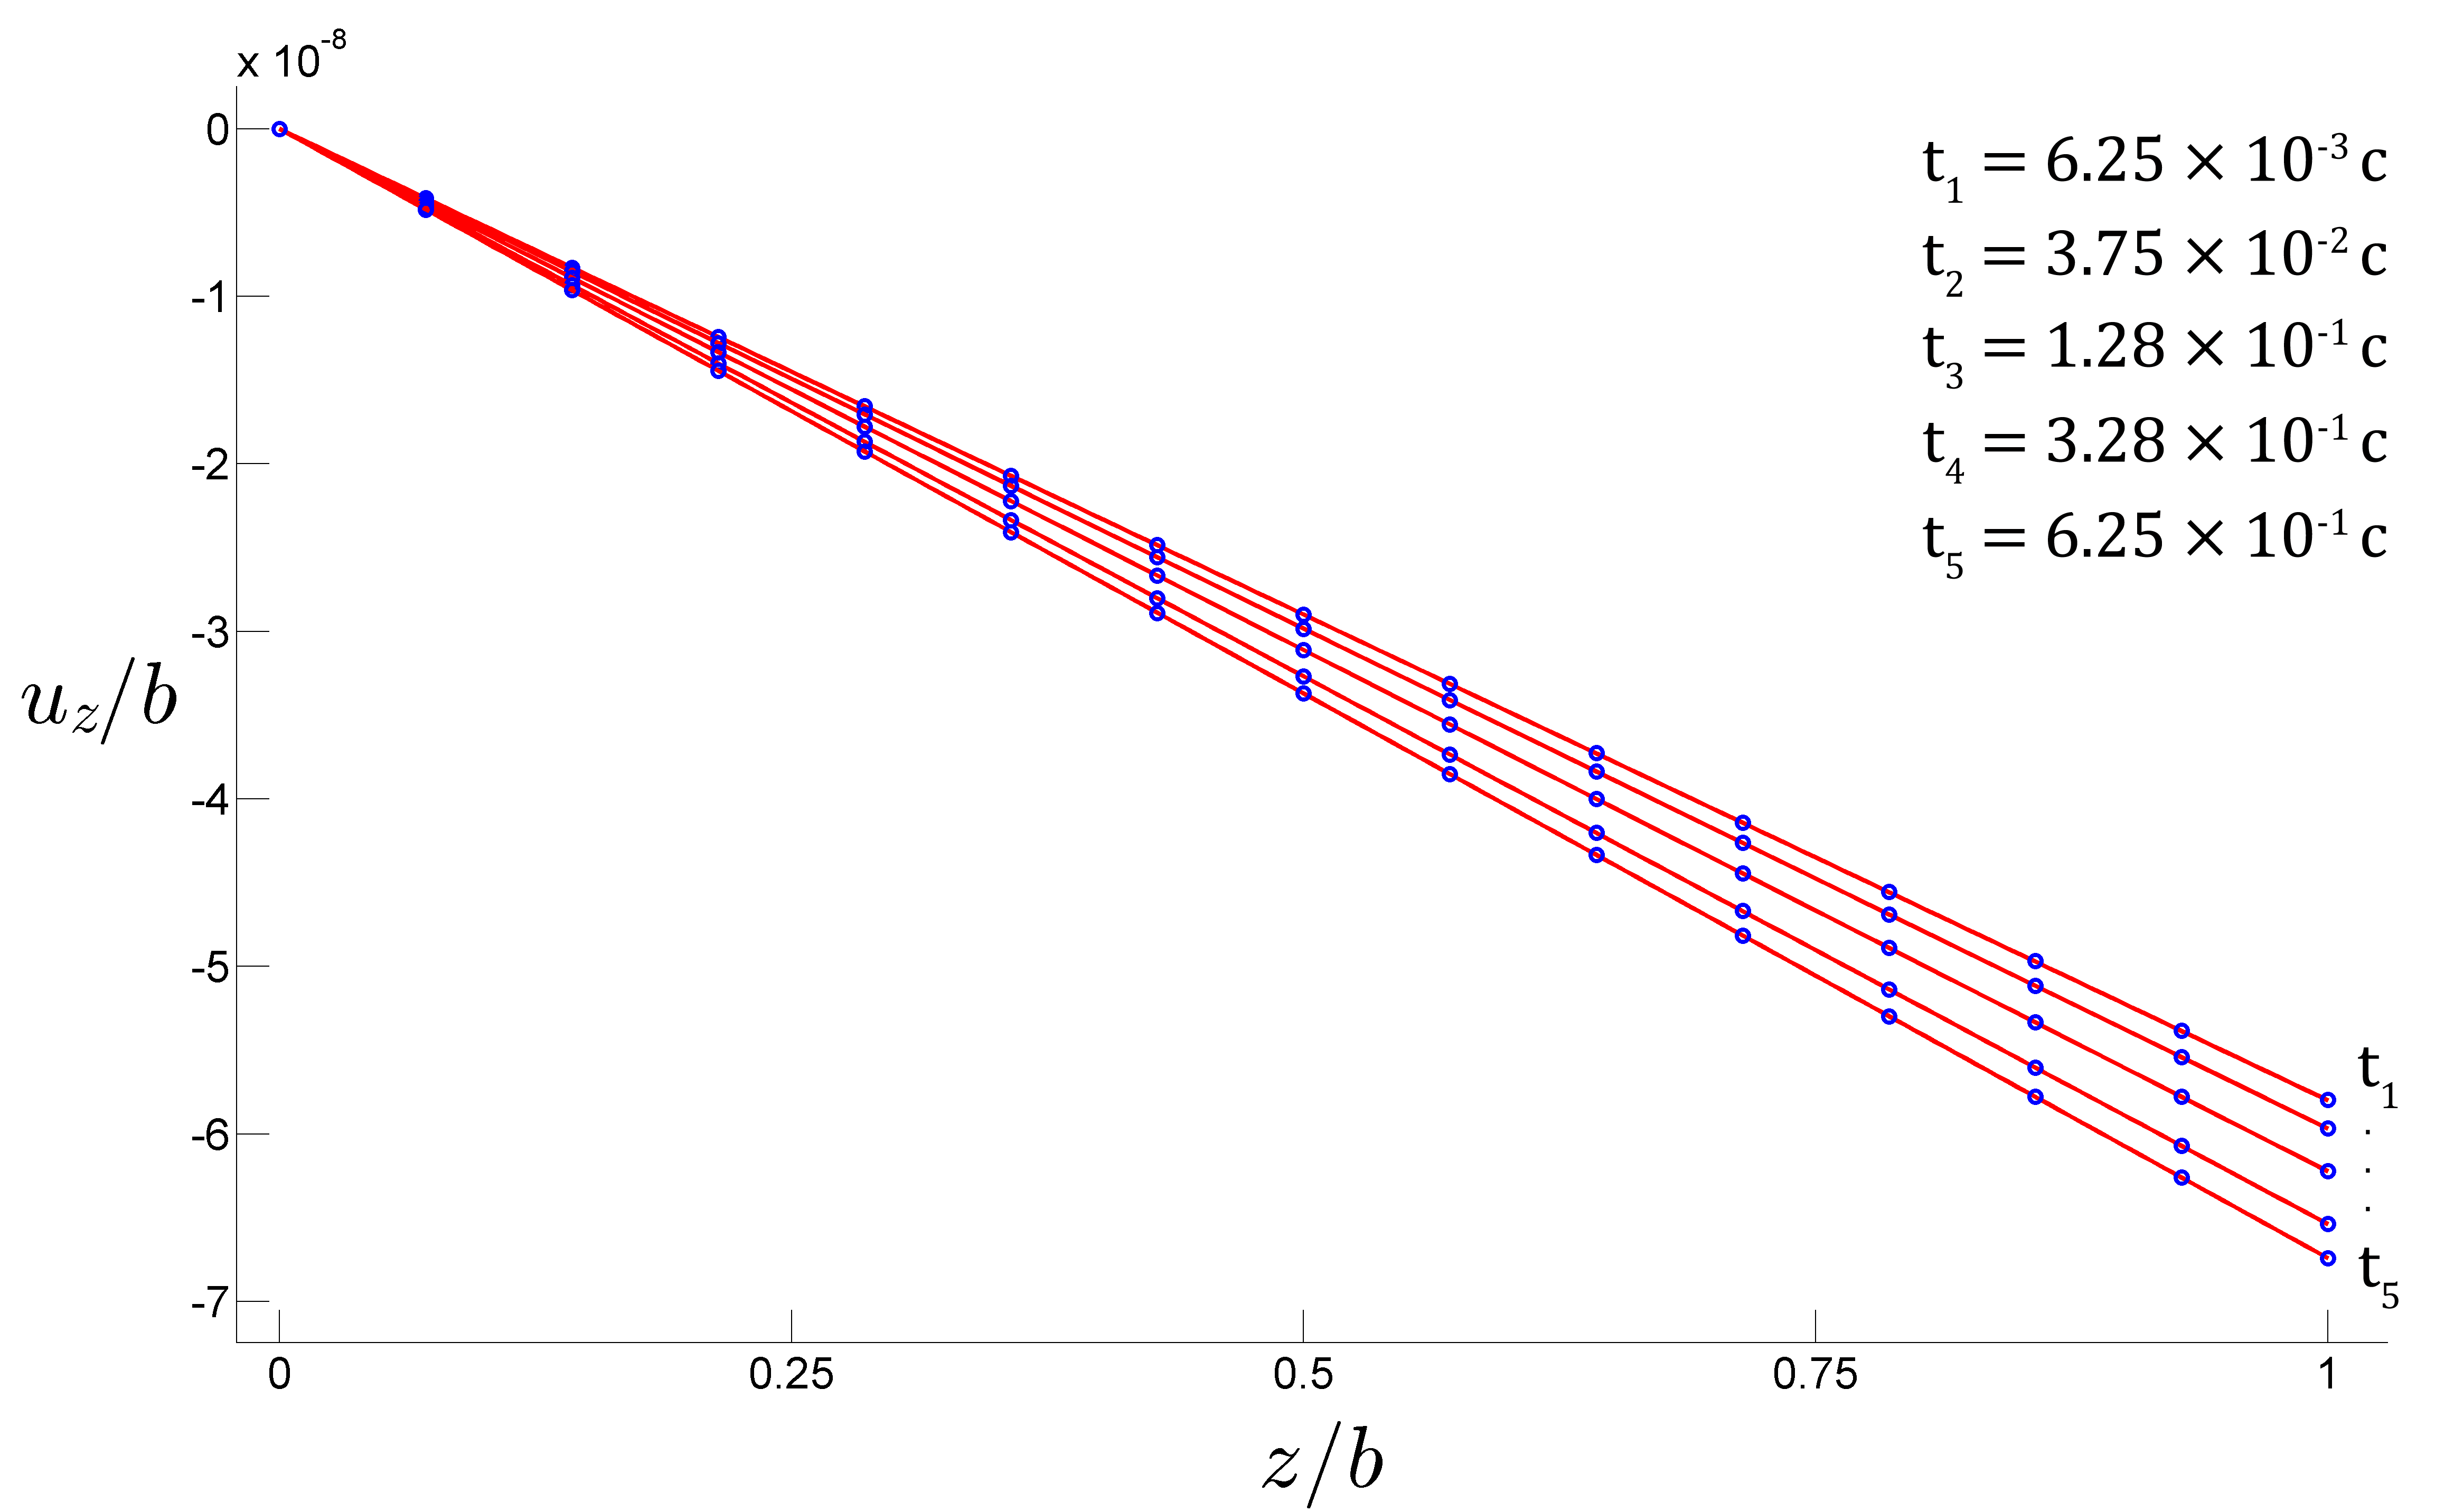
\includegraphics[width=0.85\textwidth]{./figs/uuz0M.png}
\caption{ Задача Манделя. Нормированное перемещение $u_z$ в различные моменты времени: красным цветом показано
аналитическое решение, синим~--- результаты расчета.}\label{fig:manuz}
\end{figure}
%

%
\begin{figure}[h!]
\centering
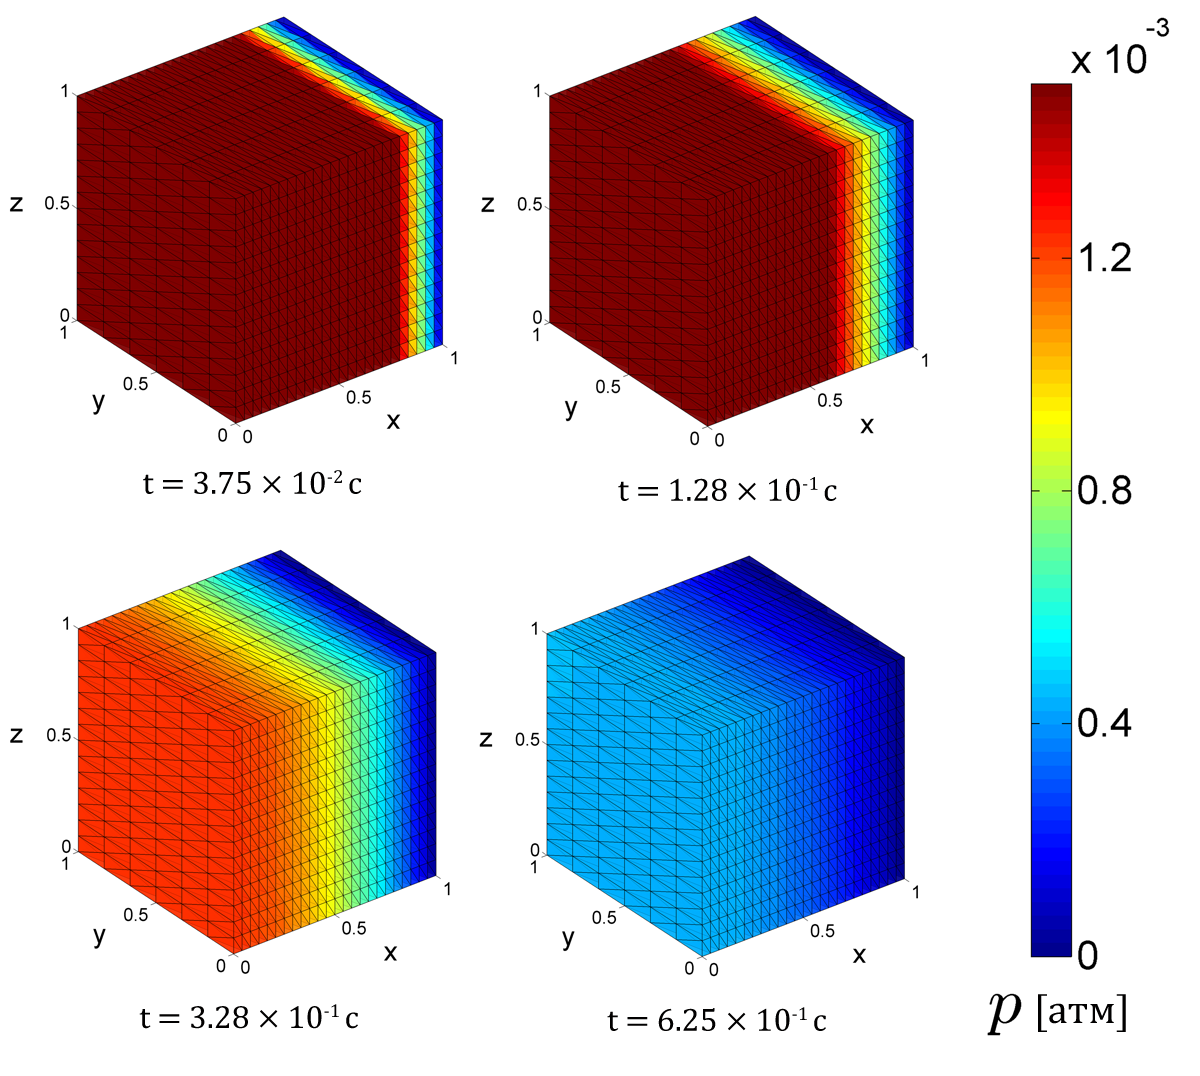
\includegraphics[width=0.73\textwidth]{./figs/prM.png}
\caption{ Задача Манделя. Распределение давления в последовательные моменты времени.}\label{fig:manpp}
\end{figure}
%

\subsection{Пороупругий пласт при наличии скважин}

Рассмотренные в предыдущих разделах постановки задач предназначены для валидации
разработанного авторами программного комплекса. Для них известно точное аналитическое решение,
но фактически данные задачи являются одномерными или двумерными.
В данном разделе рассматривается полностью трехмерная задача о перераспределении поля пластового давления
при работе двух скважин различной ориентации. К сожалению, эта задача не имеет точного аналитического решения, но иллюстрирует
возможности программного комплекса и позволяет качественно оценить достоверность полностью трехмерного моделирования задачи фильтрации в пороупругой среде в рамках разработанных алгоритмов.

Для расчетов использовалась область с линейными размерами $L_x$, $L_y$, $L_z$,
внутри которой расположены две скважины, полностью перфорирующие пласт. 
Скважины моделируются с помощью линейных источника и стока мощностью
$Q$ и $-Q$ на единицу длины. Нагнетательная скважина расположена вертикально и
проходит через точки с координатами $(L_x/3, L_y/2, 0)$ и $(L_x/3, L_y/2, L_z)$,
добывающая скважина является горизонтальной и проходит через точки
с координатами $(2L_x/3, 0, L_z/2)$ и $(2L_x/3, L_y, L_z/2)$.
Схематично постановка задачи представлена на рис.~\ref{fig:2wells}.
Конкретные значения используемых для расчетов параметров приведены в табл.~\ref{tab:2wells}.
%
\begin{figure}[h!]
\centering
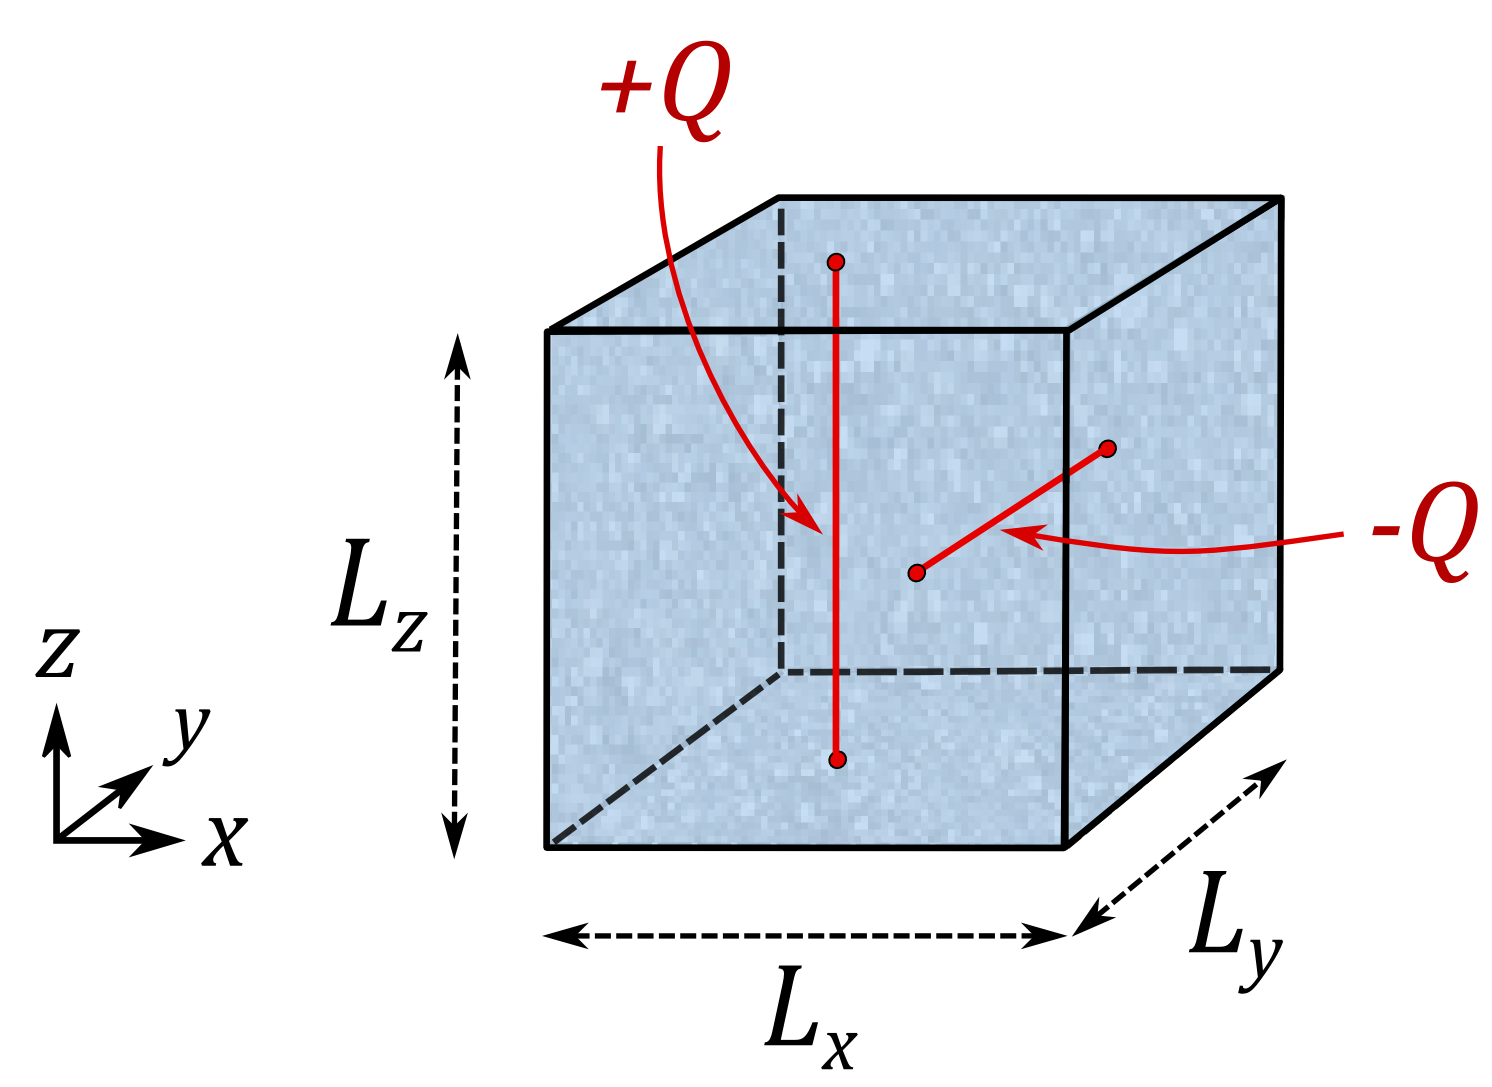
\includegraphics[width=0.65\textwidth]{./figs/2wells.png}
\caption{Схематичный вид задачи о двух скважинах.}\label{fig:2wells}
\end{figure}
% 

%%
\begin{table}[h!]
\centering
%
\renewcommand{\arraystretch}{1.5}
\renewcommand{\tabcolsep}{6 pt} 
\begin{tabular}{|c|c|c|c|c|c|c|}
\hline
$L_x$ & $L_y$ & $L_z$ & $|Q|$ & $t_{\text{start}}$ & $t_{\text{end}}$ & $\Delta t$\\
\hline
 $400.0$ м & $400.0$ м & $400.0$ м & $20.0 \text{ м}^2/\text{cутки}$ & $0.0$ ч & $20.0$ ч & $1.0$ ч\\
\hline
\end{tabular}
%
\caption{Параметры для численного расчета задачи о двух скважинах.}\label{tab:2wells}
\end{table}
%%
%

Предполагается, что пороупругая область изолирована от внешней среды.
На границе области заданы нулевые перемещения и нулевой поток, т.е. 
$\partial p/ \partial n = 0$. В качестве начального условия задавалось состояние покоя
при давлении $p = 100$ атм и нулевых перемещениях точек среды.

Для численных расчетов использовалась тетраэдральная сетка, состоящая из 
$N_{nodes} = 29791$ узлов и $N_{elems} = 162000$ прямоугольных тетраэдров со сторонами
$h_x = h_y = h_z = 13.3333$ м. 

%
\begin{figure}[t!]
\centering
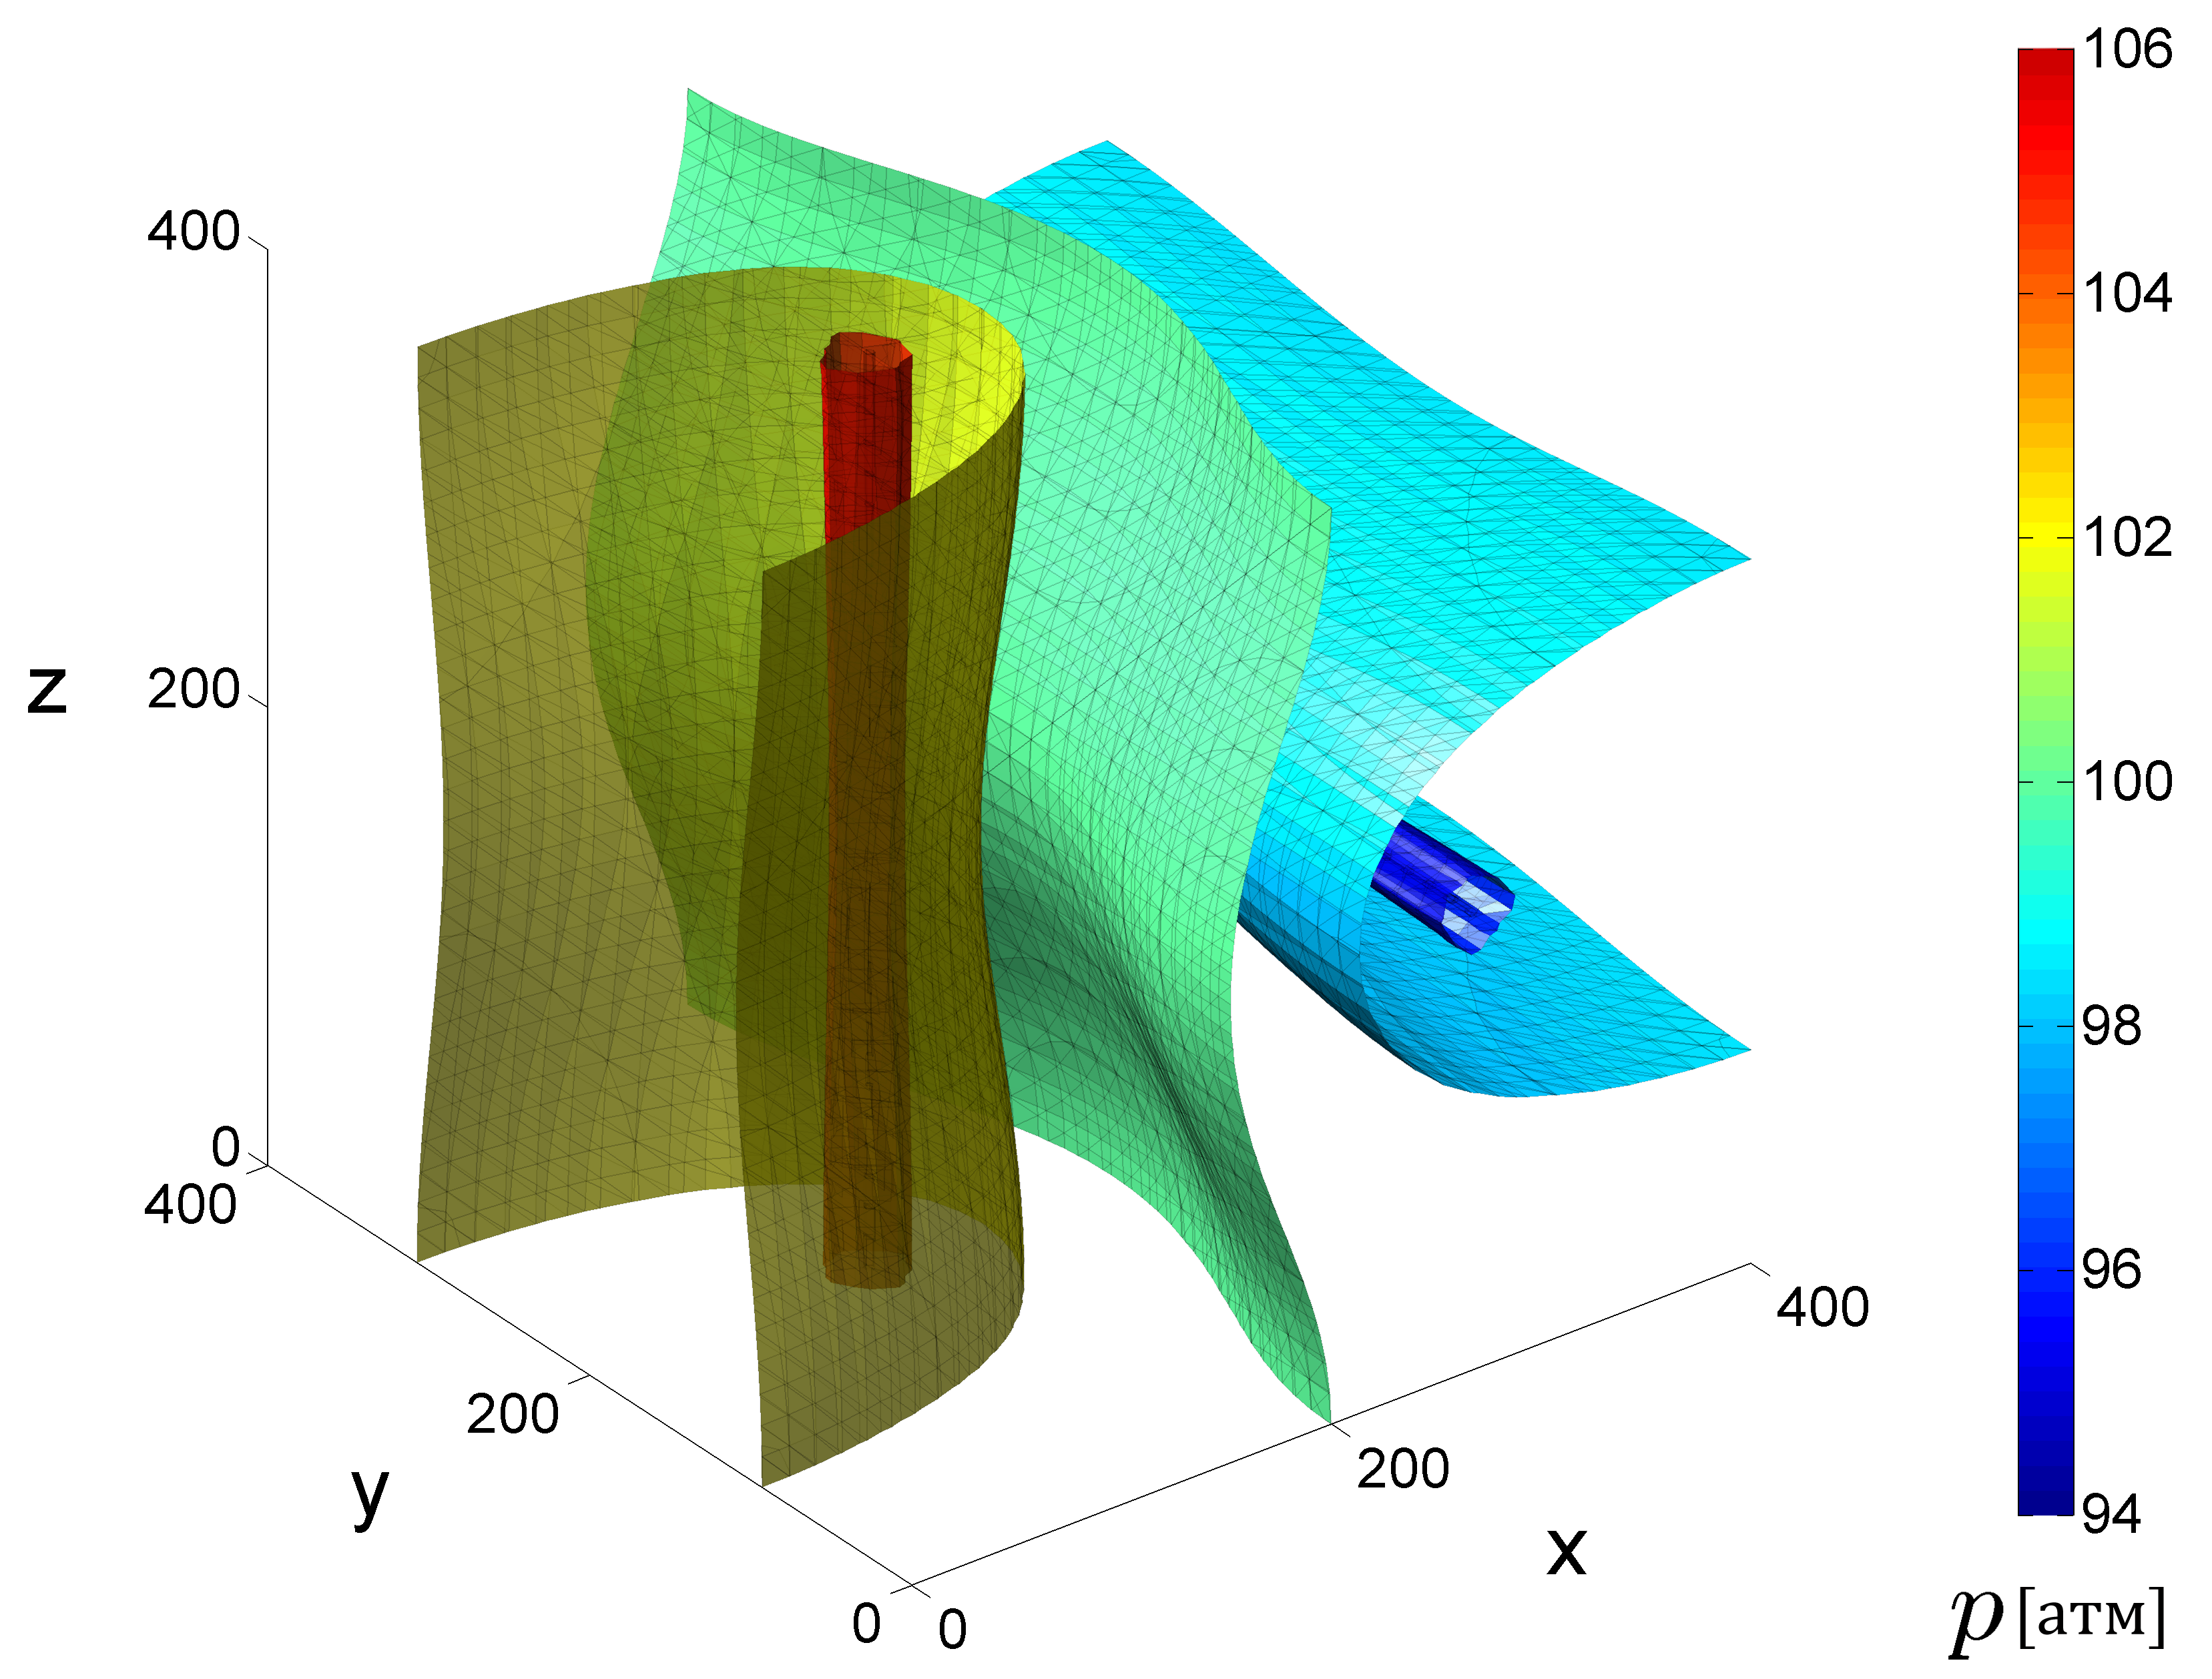
\includegraphics[width=0.8\textwidth]{./figs/iso_p.png}\\
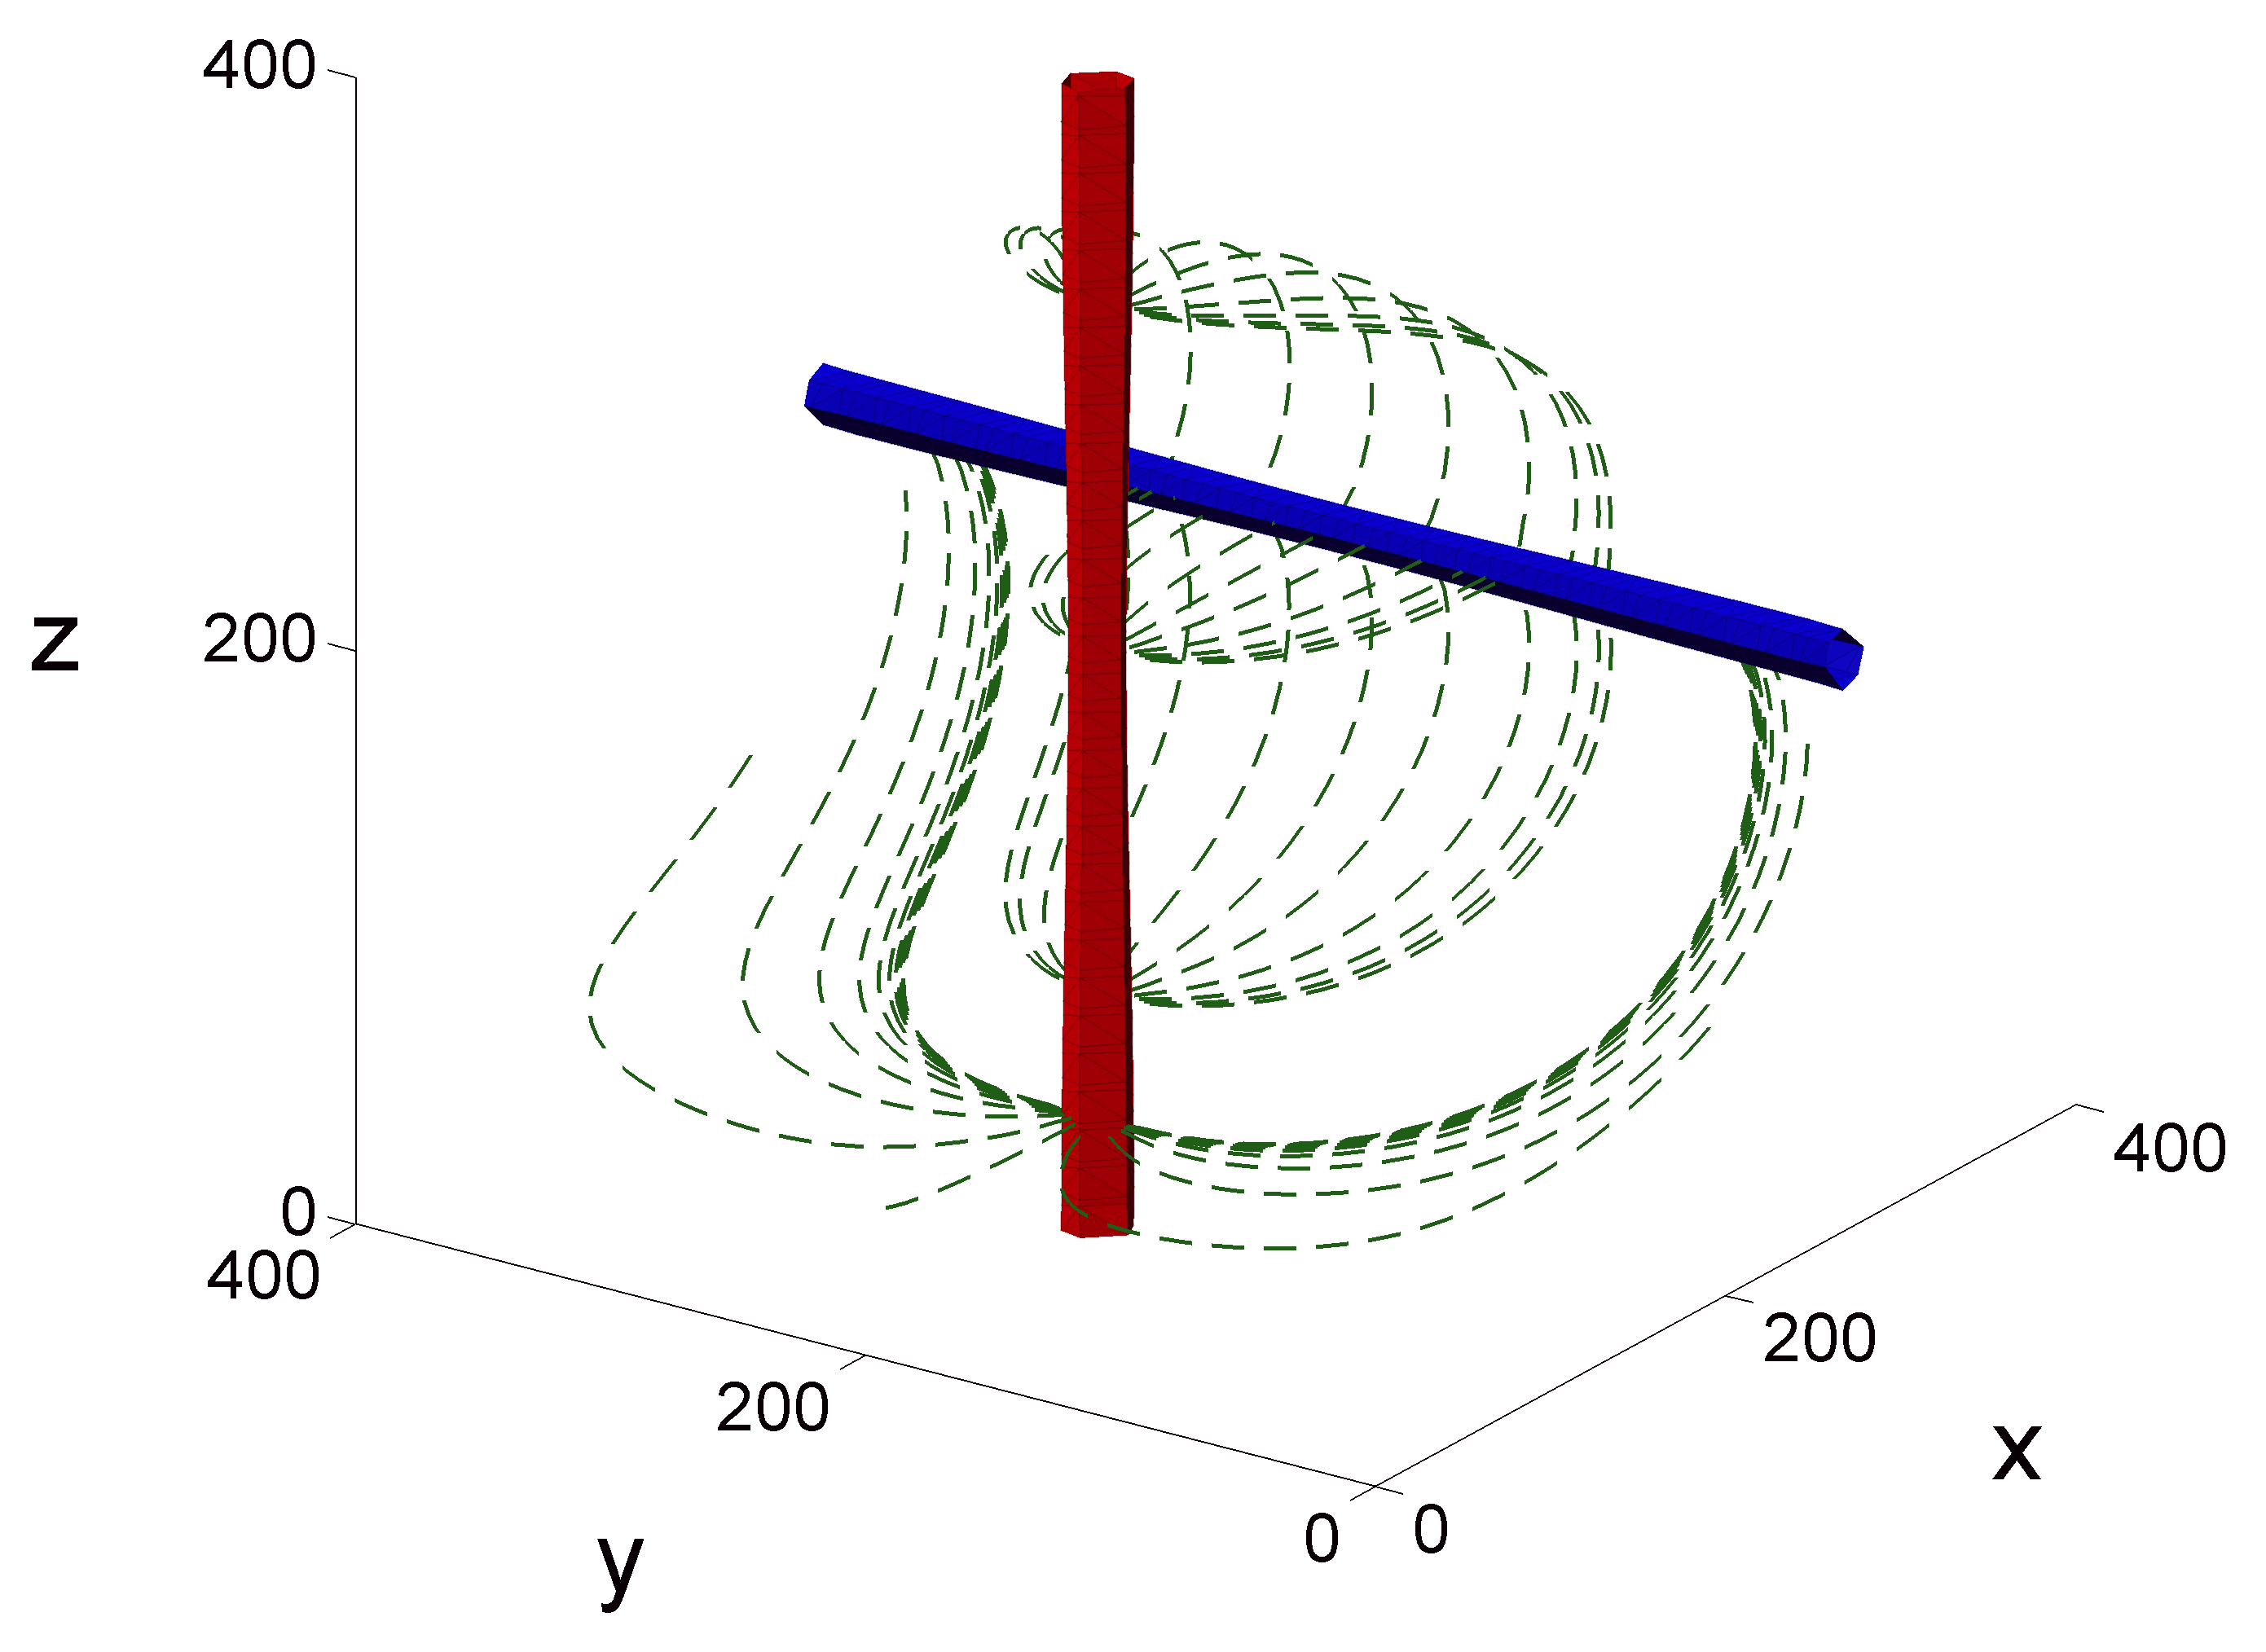
\includegraphics[width=0.8\textwidth]{./figs/str.png}
\caption{Задача о двух скважинах. Изоповерхности давления (вверху) и линии тока (внизу) в конце расчета.}\label{fig:iso}
\end{figure}
% %
% \begin{figure}[h!]
% \centering
% 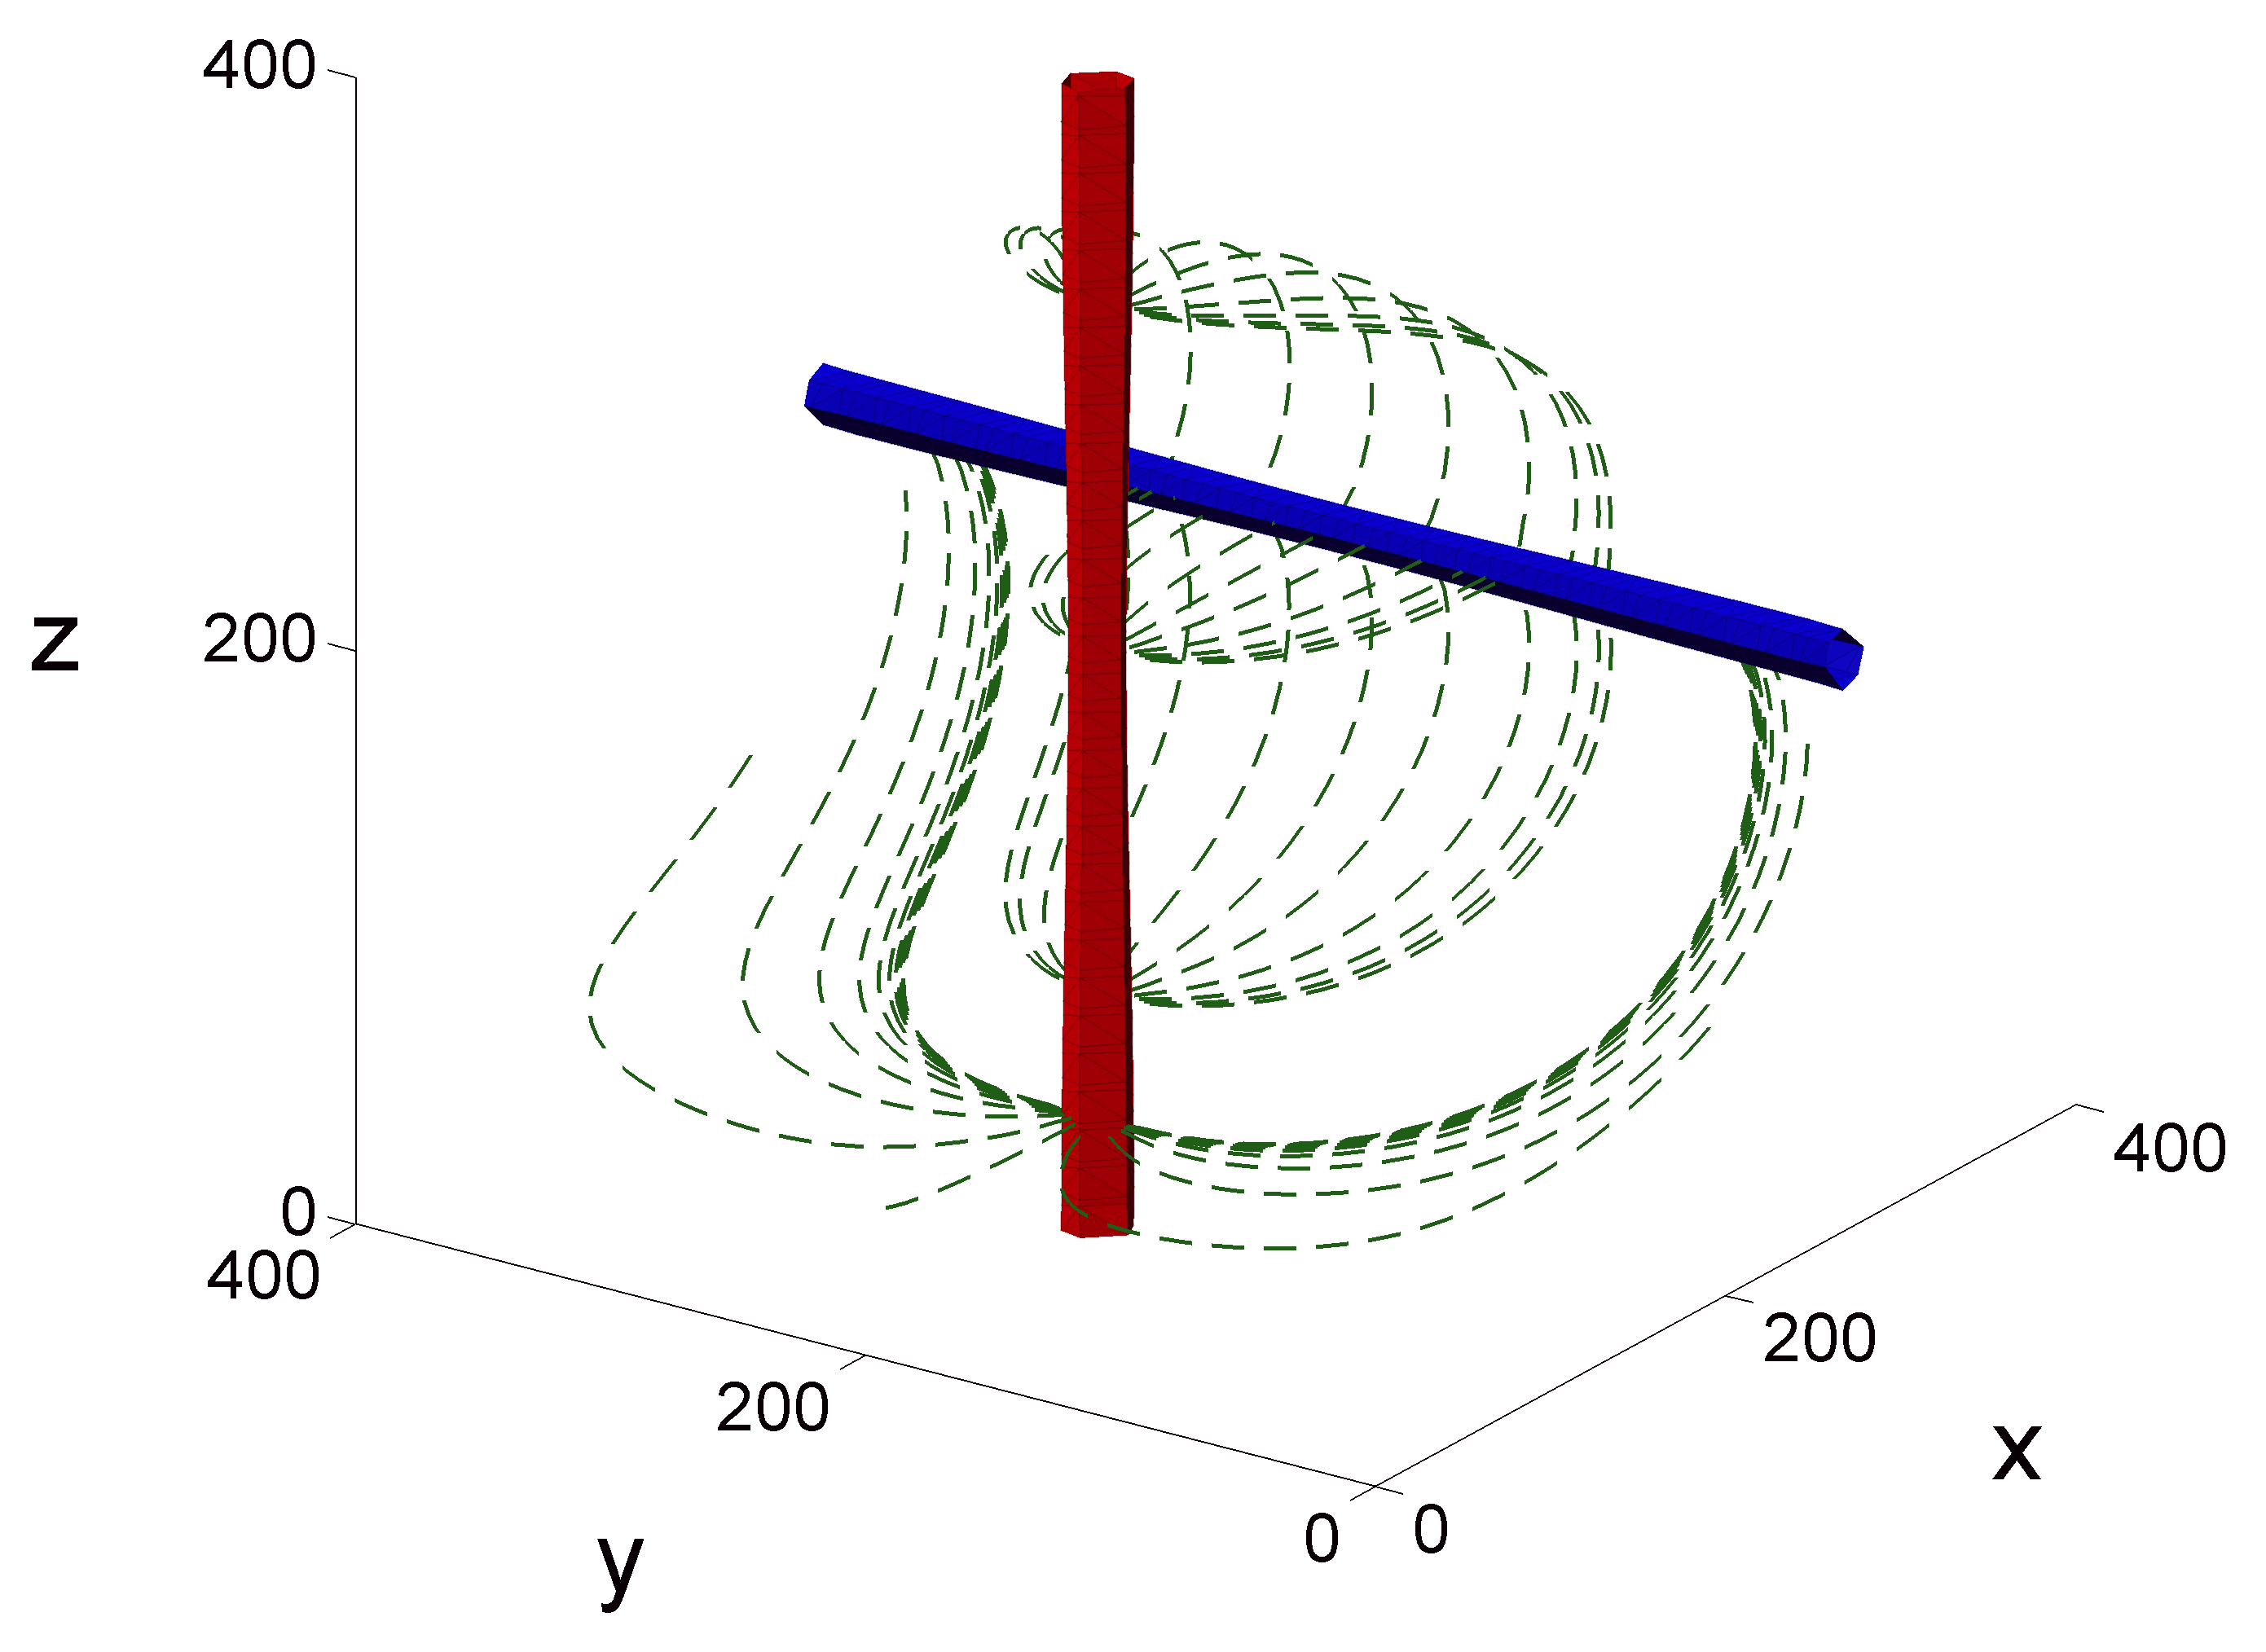
\includegraphics[width=0.83\textwidth]{./figs/str.png}
% \caption{Линии тока в конце расчета}\label{fig:str}
% \end{figure}
% 

На рис.~\ref{fig:iso} представлены несколько поверхностей уровня
порового давления (вверху) и линий тока (внизу) 
в конце моделирования при установлении псевдостационарного режима течения.
Видно, что структура течения существенно трехмерна и симметрична в силу симметричности постановки задачи.

%%%%%%%%%%%%%%%%%%%%%%%%
\settocdepth{section}

%%%%%%
\endinput
% EOF


\newpage
% Заключение
\section{Заключение}
\label{sec:finish}
%
%
% finish.tex
% 
% Заключение
% 

В настоящей работе подробно описана математическая постановка
линейной задачи пороупругости в рамках классической модели Био. 
Рассмотрен общий случай неизотермической геометрически и
физически линейной среды. Приведены основные уравнения модели и ее
определяющие соотношения. Рассмотрены основные сложности, возникающие
при численном решении задачи. 

Описанная модель и алгоритмы легли в основу ядра программного комплекса для 
математического моделирования пороупругих процессов. Работоспособность
программы иллюстрируется результатами расчета ряда распространенных тестов.
%%%%%%
\endinput
% EOF

%\newpage
% Список обозначений
%\section*{Список обозначений}
%\addcontentsline{toc}{section}{Список обозначений}
%\label{sec:result}
%\input{desc.tex}


% Литература
%

\begin{thebibliography}{1000}
\addcontentsline{toc}{section}{Литература}

% ---
% Введение

\bibitem[Азиз2004]{aziz_2004} 
Азиз Х., Сеттари Э.  Математическое
моделирование пластовых систем.  Институт компьютерных исследований,
Москва-Ижевск, 2004, 416 с.

\bibitem[Борисов2017]{borisov_2017} 
Азиз Х., Сеттари Э.  Математическое
моделирование пластовых систем.  Институт компьютерных исследований,
Москва-Ижевск, 2004, 416 с.

\bibitem[Biot1941]{biot_1941}
Борисов В.Е., Иванов А.В., Критский Б.В., Меньшов И.С., Савенков Е.Б. Численное  моделирование задач
пороупругости. Препринты ИПМ им. М.В.Келдыша. 2017. №81. 
36 с.

\bibitem[Brezzi1991]{brezzi1991}
Brezzi~F., Fortin~M. Mixed and Hybrid Finite Elements Methods.
Springer, 1991.

\bibitem[Chappele1993]{chappele1993}
Chappele~D., Bathe~K.J.
The $\inf$-$\sup$ Test //
\emph{Computers \& Structures}, 1993.
V.~47, \No~4--5, pp.~537--545.

\bibitem[Cheng1988]{cheng_1988}
Cheng~A.H-D., Detournay~E. 
A direct boundary element method for plane strain
poroelasticity // \emph{Int. J. Num. Anal. Meth. Geomech.}, 12, pp. 551--572, 1988.

\bibitem[Cleary1994]{cleary1994}
Cleary M.P., Quinn. T.S., C.J. de Pater.
Experimental Verification of Dimensional Analysis for Hydraulic Fracturing // 
SPE Production \& Facilities, November 1994.
pp.~230--238

\bibitem[Commend2004]{commend2004}
Commend~S., Truty~A.,  Zimmermann~Th.
Stabilized finite elements applied to elastoplasticity: I. Mixed displacement–pressure formulation //
\emph{Comput. Methods Appl. Mech. Engrg.}, 2004.
V.~193, pp.~3559--3586.

\bibitem[Coussy2004]{coussy_2004}
Coussy~O. Poromechanics, John Wiley and Sons, 2004.

\bibitem[Detournay1993]{detournay_1993}
Detournay~E., Cheng~ A.H.-D. 
Fundamentals of poroelasticity.
Chapter 5 in Comprehensive Rock Engineering: Principles, Practice and Projects, Vol. II, Analysis and
Design Method, ed. C. Fairhurst, Pergamon Press, 1993, pp.~113--171.

\bibitem[Ern2009]{ern2009}
Ern~A., Meunier~S.
A-posteriori error analysis of Euler-Galerkin
approximations to coupled elliptic-parabolic problems // \emph{ESAIM: M2AN}, 2009.
V.~43, \No~2, pp.~353--375.

\bibitem[Haga2012]{haga2012}
Haga~J.B., Osnes~H., Langtangen~H.P.
On the causes of pressure oscillations in low-permeable and low-compressible porous media //
\emph{Int. J. Numer. Anal. Meth. Geomech.}, 2012.
V.~36, \No~12, pp.~1507--1522.

\bibitem[Kim2009]{kim2009}
Kim~J., Tchelepi~H.A., Juanes~R. Stability, Accuracy and Efficiency of Sequential Methods
for Coupled Flow and Geomechanics // SPE Paper 119084, 2009. 

\bibitem[Kim2010]{kim2010}
Kim~J. Sequentual Methods for Coupled Geomechanics and Multiphase Flow //
PhD Thesis, Stanford University, 2010, 274~p.

\bibitem[Lewis1998]{lewis1998}
Lewis~R.W., Schrefler~B.A. The Finite Element
Method in the Static and Dynamic Deformation and Consolidation in
Porous Media. J. Wiley, Chichester, 2nd ed., 1998.

\bibitem[Mandel1953]{mandel_1953}
Mandel~J. Consolidation des sols (itude mathimatique) // \emph{Gbotechnique}, 1953, pp.~287--299.

\bibitem[Murad1996]{murad1996}
Murad~M.A., Thomee~V., Loula~A.F.D.
Asymptotic Behavior of Semidiscrete Finite-Element Approximations of Biot's Consolidation
Problem // \emph{SIAM Journal on Numerical Analysis}, 1996.
V.~33, \No~3, pp.~1065--1083.

\bibitem[Noorishad1982]{noorishad1982}
Noorishad~J., Ayatollahi~M.S., Witherspoon~P.A.
A Finite-Element Method for Coupled
Stress and Fluid Flow Analysis in
Fractured Rock Masses // \emph{J. Rock Mech. Min. Sol \& Geomech.}, 1982.
V.~19, pp.~185--193.

\bibitem[Philips2005]{philips2005}
Philips~B.A.
Finite Element Methods in Linear Poroelasticity:
Theoretical and Computational Results // PhD Thesis, The University of Texas at Austin, 2005, 284~p.

\bibitem[Philips2009]{philips2009}
Phillips~P.J., Wheeler~M.F.
Overcoming the problem of locking in linear elasticity
and poroelasticity: an heuristic approach // \emph{Comput. Geosci.}, 2009.
V.~13, pp.~5--12.

\bibitem[Preisig2011]{preisig2011}
Preisig~M., Pr\'vost~J.H.
Stabilization procedures in coupled poromechanics problems:
A critical assessment // \emph{Int. J. Numer. Anal. Meth. Geomech.}, 2011.
V.~35, pp.~1207--1225.

\bibitem[Showalter2000]{showalter2000}
Showalter R.E.
Diffusion in Poro-Elastic Media // \emph{Journal of Mathematical Analysis and Applications}, 2000.
V.~251, \No~1, pp.~310--340.

\bibitem[Terzaghi1996]{terzaghi_1996}
Terzaghi~K. Soil mechanics in engineering practice. John Wiley \& Sons, 1996.

\bibitem[Trimonova2017]{trimonova2017}
Trimonova~M., Baryshnikov~N., Zenchenko~E., Zenchenko~P., Turuntaev~S.
The Study of the Unstable Fracure Propagation in the Injection Well: Numerical and Laboratory Modeling. // 
Society of Petroleum Engineers, 2017, October 16. 
Conference paper. 187822-MS. 

\bibitem[Trimonova2018]{trimonova2018}
Trimonova~M., Baryshnikov~N., Zenchenko~E., Zenchenko~P., Turuntaev~S., Aigozhieva~A.
Estimation of the Hydraulic Fracture Propagation Rate in the Laboratory Experiment. // 
Physical and Mathematical Modeling of Earth and Environment Processes. 2018.

\bibitem[Vermeer1981]{vermeer1981}
Vermeer~P.A., Verruijt~A.
An Accuracy condition for Consolidation by Finite Elements //
\emph{Int. J. Numer. Anal. Meth. Geomech.}, 1981. V.~5, pp.~1--14.

\bibitem[Wan2002]{wan2002}
Wan~J. Stabilized Finite Element Method for Coupled Geomechanics and  Multiphase Flow //
PhD Thesis, Stanford Univeristy, 2002, 180~p.

\bibitem[Wang2000]{wang_2000}
Wang~H.F. Theory of Linear Poroelasticity, Princeton University Press, 2000.

\bibitem[White2008]{white2008}
White~J.A., Borja~R.I. 
Stabilized low-order finite elements for coupled solid-deformation/fluid-diffusion and their application to fault zone transients //
\emph{Comput. Methods Appl. Mech. Engrg.}, 2008.
V.~197, \No~49--50, pp.~4353--4366.

\bibitem[Wieners2003]{wieners2003} 
Wieners~C.
Taylor-Hood elements in 3D // in Analysis and Simulation of Multifield Problems, 
Wolfgang L. Wendland, Messoud Efendiev, Lecture Notes in Applied and Computational Mechanics, Springer, 2003.
V.~12, 381~p.

\bibitem[Xia2009]{xia2009}
Xia~K., Masud~A.
A stabilized finite element formulation for finite deformation
elastoplasticity in geomechanics // \emph{Computers and Geotechnics}, 2009.
V.~36, pp.~396--405.

\bibitem[Zheng2003]{zheng2003}
Zheng~Y., Burridge~R., Burns~D.
Reservoir Simulation with the Finite Element Method Using Biot Poroelastic Approach // 
Earth Resources Laboratory Industry Consortia Annual Report 2003-11, 
Massachusetts Institute of Technology. Earth Resources Laboratory, 2003, 20~p.

%%%%%%%%%%%%%%%%%%%%%%%%
\end{thebibliography}

\endinput
%%%%
% EOF


%%%%%%%%%%%%%%%%%%%%%%%%%%%%%%%%%%%%%%%
%%%%%%%%%%%%%%%%%%%%%%%%%%%%%%%%%%%%%%%

%%%%%%%%%%%%%%%%%%%%%%%%%%%%%%%%%%%%%%%
%\newpage

%%%%%%%%
\end{document}
% EOF
